% sage_latex_guidelines.tex V1.20, 14 January 2017

\documentclass[Afour,sageh,times]{sagej}
\usepackage[inline]{enumitem}
\usepackage{amsmath}
% \usepackage{cite}
\usepackage{amssymb,amsfonts}
\usepackage[ruled,vlined]{algorithm2e}
\usepackage{graphicx}
\usepackage{subfloat}
\usepackage{textcomp}
\usepackage{xcolor}
\usepackage{verbatim} 
\usepackage{mathrsfs}
\usepackage{subfigure}
\usepackage{empheq}
\usepackage{courier}
\usepackage{lipsum}
\usepackage{comment}
\usepackage{gensymb}
\usepackage{mathtools}
\usepackage{bm}
\usepackage{ wasysym } % For /ocircle
\usepackage{soul}
\usepackage[table]{xcolor}
% \usepackage{moreverb,url}

\usepackage[colorlinks,bookmarksopen,bookmarksnumbered,citecolor=red,urlcolor=red]{hyperref}

\newcommand\BibTeX{{\rmfamily B\kern-.05em \textsc{i\kern-.025em b}\kern-.08em
T\kern-.1667em\lower.7ex\hbox{E}\kern-.125emX}}

\newcommand{\qm}[1]{{\textcolor{cyan}{\textbf{[Qian]} #1}}}
\newcommand{\hkc}[1]{{\textcolor{blue}{[HKG]\emph{\bf#1 }}}}
\newcommand{\todo}{\textcolor{red}{TODO }}
\long\def\revised#1{{\color{blue}#1}}

% Caligraphic

\newcommand{\call}{\mathcal}

\def\cA{{\call A}}
\def\cB{{\call B}}
\def\cC{{\call C}}
\def\cD{{\call D}}
\def\cE{{\call E}}
\def\cF{{\call F}}
\def\cH{{\call H}}
\def\cI{{\call I}}
\def\cJ{{\call J}}
\def\cK{{\call K}}
\def\cL{{\call L}}
\def\cM{{\call M}}
\def\cN{{\call N}}
\def\cO{{\call O}}
\def\cP{{\call P}}
\def\cQ{{\call Q}}
\def\cR{{\call R}}
\def\cS{{\call S}}
\def\cT{{\call T}}
\def\cU{{\call U}}
\def\cV{{\call V}}
\def\cW{{\call W}}
\def\cX{{\call X}}
\def\cY{{\call Y}}
\def\cZ{{\call Z}}

\newcommand{\integers}{\mathbb{Z}}
\newcommand{\naturals}{\mathbb{N}}

\newcommand{\ap}{AP}
\newcommand{\true}{{\tt{True}}}
\newcommand{\false}{{\tt{False}}}
\newcommand{\var}{\pi}
\newcommand{\inp}{\cI}
\newcommand{\inpsyms}{\inp_\textrm{c}}
\newcommand{\inpuser}{\inp_\textrm{u}}
\newcommand{\inpuserprov}{\inp_\textrm{user}}
\newcommand{\inpcen}{\inp_{\textrm{robot}}}
\newcommand{\inpcentrans}{\inp_{\textrm{robot}}^{\textrm{trans}}}
\newcommand{\inpcenorien}{\inp_{\textrm{robot}}^{\textrm{orien}}}
\newcommand{\inpterrain}{\inp_{\textrm{terrain}}}
\newcommand{\inpterrainbool}{\inp_{\textrm{terrain}}^{\cB}}
\newcommand{\inpterrainint}{\cE_\naturals}
\newcommand{\terrainexprs}{E}
\newcommand{\inpstatesterrainexpr}{2^{\inpterrain}}
\newcommand{\inpstatesterrainexprposs}{\dom_{\textrm{terrain}}^{\textrm{poss}}}

\newcommand{\inpstateterrainexpr}{\inpstatesterrain}
\newcommand{\inprequest}{\inp_{\textrm{req}}}
\newcommand{\inprequesttrans}{\inp_{\textrm{req}}^{\textrm{trans}}}
\newcommand{\inprequestorien}{\inp_{\textrm{req}}^{\textrm{orien}}}
\newcommand{\tvar}[2]{n_{#1}^{#2}}
\newcommand{\cells}{\cC}
\newcommand{\xcells}{\cX}
\newcommand{\ycells}{\cY}
\newcommand{\out}{\cO}
\newcommand{\skillcustom}[1]{\skill_{#1}}
\newcommand{\skillprecustom}[1]{\Sigma_{#1}^{\textrm{pre}}}
\newcommand{\skillpostcustom}[1]{\Sigma_{#1}^{\textrm{post}}}
\newcommand{\skill}{o}
\newcommand{\skillpre}{\skillprecustom{\skill}}
\newcommand{\skillpost}{\skillpostcustom{\skill}}
\newcommand{\skillpretrans}{\skillprecustom{\skill_{\textrm{trans}}}}
\newcommand{\skillposttrans}{\skillpostcustom{\skill_{\textrm{trans}}}}
\newcommand{\skillpreorien}{\skillprecustom{\skill_{\textrm{orien}}}}
\newcommand{\skillpostorien}{\skillpostcustom{\skill_{\textrm{orien}}}}

\newcommand{\dom}{\Sigma}
\newcommand{\statevar}{\sigma}
\newcommand{\inpstate}{\statevar_\inp}
\newcommand{\inpstates}{\dom_\inp}
\newcommand{\inpstateterrain}{\statevar_{\textrm{terrain}}}
\newcommand{\inpstateterrainbool}{\statevar_{\textrm{terrain}}^{\cB}}

\newcommand{\inpstateterrainint}{\statevar_{\inpterrainint}}
\newcommand{\inpstatesterrain}{\dom_{\textrm{terrain}}}
\newcommand{\inpstatesterrainint}{\dom_{\inpterrainint}}
\newcommand{\inpstatecen}{\statevar_{\textrm{robot}}}
\newcommand{\inpstatescen}{\dom_{\textrm{robot}}}
\newcommand{\inpstaterequest}{\statevar_{\textrm{req}}}
\newcommand{\inpstatesrequest}{\dom_{\textrm{req}}}
\newcommand{\inpstatesrequestposs}{\dom_{\textrm{req}}^{\textrm{poss}}}
\newcommand{\inpstateterrainposs} {\Sigma_{\inpterrain}^{\textrm{poss}}}

%%%% Ref %%%%
\newcounter{examplecounter}
\setcounter{examplecounter}{0}

\newcommand{\examplelabel}[1]{%
  \refstepcounter{examplecounter}%
  \label{#1}%
  \theexamplecounter%
}

\newcounter{problemcounter}
\setcounter{problemcounter}{0}

\newcommand{\problemlabel}[1]{%
  \refstepcounter{problemcounter}%
  \label{#1}%
  \theproblemcounter%
}

\newcounter{defcounter}
\setcounter{defcounter}{0}

\newcommand{\deflabel}[1]{
    \refstepcounter{defcounter}%
    \label{#1}%
    \thedefcounter%
}

%%%%%%%%%%%%%%%%%%%%%%%%%%
%%%% Spec related %%%%
\newcommand{\envspec}{\varphi_\textrm{e}}
\newcommand{\boolspec}{\varphi_{b}}
\newcommand{\sysspec}{\varphi_\textrm{s}}
\newcommand{\envinit}{\varphi_\textrm{e}^\textrm{i}}
\newcommand{\sysinit}{\varphi_\textrm{s}^\textrm{i}}
\newcommand{\alphainit}{\varphi_\alpha^\textrm{i}}
\newcommand{\envsafety}{\varphi_\textrm{e}^\textrm{t}}
\newcommand{\envterrain}{\varphi_\textrm{e}^\textrm{terrain}}
\newcommand{\alphasafety}{\varphi_\alpha^\textrm{t}}
\newcommand{\envsafetyvio}{\varphi_\textrm{violated}}
\newcommand{\envsafetynothard}{\varphi_\textrm{e}^\textrm{t,skill}}
\newcommand{\envsafetyhard}{\varphi_\textrm{e}^\textrm{t,hard}}
\newcommand{\alphasafetynothard}{\varphi_\alpha^\textrm{t,skill}}
\newcommand{\alphasafetyhard}{\varphi_\alpha^\textrm{t,hard}}
\newcommand{\envsafetyharduser}{\varphi_\textrm{e}^\textrm{t,user}}
\newcommand{\syssafety}{\varphi_\textrm{s}^\textrm{t}}
\newcommand{\syssafetynothard}{\varphi_\textrm{s}^\textrm{t,skill}}
\newcommand{\syssafetyhard}{\varphi_\textrm{s}^\textrm{t,hard}}
\newcommand{\syssafetyuser}{\varphi_\textrm{s}^\textrm{t,user}}
\newcommand{\syssafetycontinue}{\varphi_\textrm{s}^\textrm{t,continue}}
\newcommand{\syssafetychoose}{\varphi_\textrm{s}^\textrm{t,choose}}
\newcommand{\envlive}{\varphi_\textrm{e}^\textrm{g}}
\newcommand{\syslive}{\varphi_\textrm{s}^\textrm{g}}
\newcommand{\alphalive}{\varphi_\alpha^\textrm{g}}
\newcommand{\changecons}{\varphi_\textrm{poss-changes}}
\newcommand{\notallowedrepair}{\varphi_\textrm{disallow}}
\newcommand{\disallowedtrans}{\notallowedrepair}
\newcommand{\specsafe}{\spec^\textrm{t}}
\newcommand{\speclive}{\spec^\textrm{g}}
\newcommand{\alphasafetybool}[1]{\specsafe_{\textrm{a}, #1}}
\newcommand{\alphalivebool}[1]{\speclive_{\textrm{a}, #1}}

\newcommand{\spec}{\varphi}
\newcommand{\spectask}{\spec_{\textrm{task}}}
\newcommand{\specrelax}{\spec_{\textrm{relax}}}
\newcommand{\specrepair}{\spec_{\textrm{repair}}}
\newcommand{\oldspec}{\varphi_{\textrm{old}}}
\newcommand{\newspec}{\varphi_{\textrm{new}}}
\newcommand{\psicheck}{\psi_i^{\textrm{check}}}
\newcommand{\envrelaxhard}{\psi_{\textrm{r}}^{\textrm{hard}}}
\newcommand{\envrelaxnothard}{\psi_{\textrm{r}}^{\textrm{skill}}}
\newcommand{\trace}{\tau}
\newcommand{\traceinf}{\tau_{\textrm{inf}}}
\newcommand{\tracefin}{\tau_{\textrm{fin}}}


%%%%%%%%%%%%%%%%%%%%%%%%%%%%%%%%%

%%%% Functions %%%%
\newcommand{\downright}[3]{\textit{#1}_{#2}(#3)}
\newcommand{\form}[2]{\downright{form}{#1}{#2}}
\newcommand{\formplain}{\textit{form}}
\newcommand{\range}[1]{[#1]}

%%%% Repair %%%%
\newcommand{\winning}{Z}
\newcommand{\strategy}{\cA}

\newcommand{\grounding}{\textrm{G}}
% \newcommand{\groundingreg}{\textrm{G}_\reg}
\newcommand{\inversegrounding}{\grounding^{-1}}
\newcommand{\ps}{\cZ}
\newcommand{\physicalstate}{z}
\newcommand{\reals}{\mathbb{R}}

\newcommand{\vg}[1]{\bm{#1}}
\renewcommand{\v}[1]{\mathbf{#1}}

%\usepackage[usenames,dvipsnames]{xcolor}
\newcommand{\ye}[1]{\textbf{\textcolor{red}{Ye: #1}}}
\newcommand{\ziyi}[1]{\textbf{\textcolor{blue}{Ziyi: #1}}}

\def\volumeyear{2026}

\begin{document}

\runninghead{Zhou et al.}

\title{Physically-Feasible Reactive Synthesis for Terrain-Adaptive Locomotion}

\author{Ziyi Zhou\affilnum{1}, Qian Meng\affilnum{2}, Hadas Kress-Gazit\affilnum{2}, and Ye Zhao\affilnum{1}}

\affiliation{\affilnum{1}Georgia Institute of Technology, Atlanta, GA, USA\\
\affilnum{2}Cornell University, Ithaca, NY, USA}

\corrauth{Ye Zhao, Georgia Institute of Technology, Atlanta, GA 30332, USA.}

\email{ye.zhao@me.gatech.edu}

\setcounter{secnumdepth}{3}

%%%%%%%%% Abstract %%%%%%%%
\begin{abstract}
% We propose an integrated planning framework for quadrupedal locomotion over dynamically changing, unforeseen terrains.
% Existing 
% approaches either 
% rely on heuristics for instantaneous foothold selection--compromising safety and versatility--or 
% solve expensive trajectory optimization problems
% with complex terrain features and long time horizons.
% In contrast,
% our framework leverages reactive synthesis to 
% generate correct-by-construction controllers
% at the symbolic level, 
% and mixed-integer convex programming (MICP) 
% for dynamic and physically feasible 
% footstep planning 
% for each symbolic transition.
% We use a high-level manager to reduce the large state space
% in synthesis
% by incorporating local environment information, improving synthesis scalability.
% To handle specifications that cannot be met due to dynamic infeasibility,
% and to minimize costly
% MICP solves,
% we leverage a 
% symbolic repair process to 
% generate only necessary
% symbolic transitions.
% During online execution, 
% re-running the MICP with real-world terrain data, along with runtime symbolic repair,
% bridges the gap between offline synthesis and online execution.
% Through extensive simulation and hardware experiments, we demonstrate
% our framework's capabilities to discover missing locomotion skills and 
% react promptly
% in safety-critical environments, such as scattered stepping stones and rebars. Code and experimental videos are available at \url{https://synthesis-micp.github.io/}.
We present an integrated planning framework for quadrupedal locomotion over \revised{discrete, unforeseen terrain configurations revealed at runtime}.
Existing methods often depend on heuristics for real-time foothold selection---limiting robustness and adaptability---or rely on computationally intensive trajectory optimization across complex terrains and long horizons. In contrast, our approach combines reactive synthesis for generating correct-by-construction symbolic-level controllers with mixed-integer convex programming (MICP) for physically feasible footstep planning during each symbolic transition. To reduce the reliance on costly MICP solves and accommodate specifications that may be violated due to physical infeasibility, we adopt a symbolic repair mechanism that selectively generates only the required symbolic transitions. During execution, real-time MICP replanning based on actual terrain data, runtime symbolic repair, \revised{kinematic-feasibility re-targeting, and a delay-aware coordination scheme} enable seamless bridging between offline synthesis and online operation. Through extensive simulation and hardware experiments, we validate the framework's ability to identify missing locomotion skills and respond effectively in safety-critical environments, including scattered stepping stones and rebar scenarios. Code and experimental videos are available at \url{https://synthesis-micp.github.io/}.
\end{abstract}

% \begin{abstract}
% This paper describes the use of the \LaTeXe\
% \textsf{\journalclass} class file for setting papers to be
% submitted to a \textit{SAGE Publications} journal.
% The template can be downloaded \href{http://www.uk.sagepub.com/repository/binaries/SAGE LaTeX template.zip}{here}.
% \end{abstract}

\keywords{Legged Robots, Optimization and Optimal Control,
Formal Methods in Robotics and Automation}

\maketitle


%%%%%%%%% Introduction %%%%%%%%
\section{Introduction}
Terrain-adaptive locomotion is essential for enhancing the mobility of legged robots and moving beyond blind walking strategies \citep{di2018dynamic,kim2019highly, zhou2022momentum}. Many existing methods achieve terrain adaptability by adjusting footholds around a nominal trajectory in real time \citep{fankhauser2018robust,grandia2023perceptive}. To further boost traversability, some approaches have explored variable gait patterns. In \citep{Park2015OnlinePF, kim2020vision,gilroy2021autonomous}, jumping motions are precomputed offline and triggered heuristically upon detecting obstacles. Other methods embed gait switching—such as transitions from walking to jumping—within simplified dynamics models during trajectory sampling \citep{norby2020fast}, or rely on pre-trained classifiers to assess feasibility \citep{chignoli2022rapid}. However, despite the importance of safety in high-risk settings such as disaster zones and construction sites, relatively few works address formal safety guarantees for agile, variable-gait locomotion \citep{zhao2022reactive,shamsah2023integrated} that fully account for the robot's physical limitations.

%%%% Fig.2 System architecture %%%%
\begin{figure}[t]
    \centering
    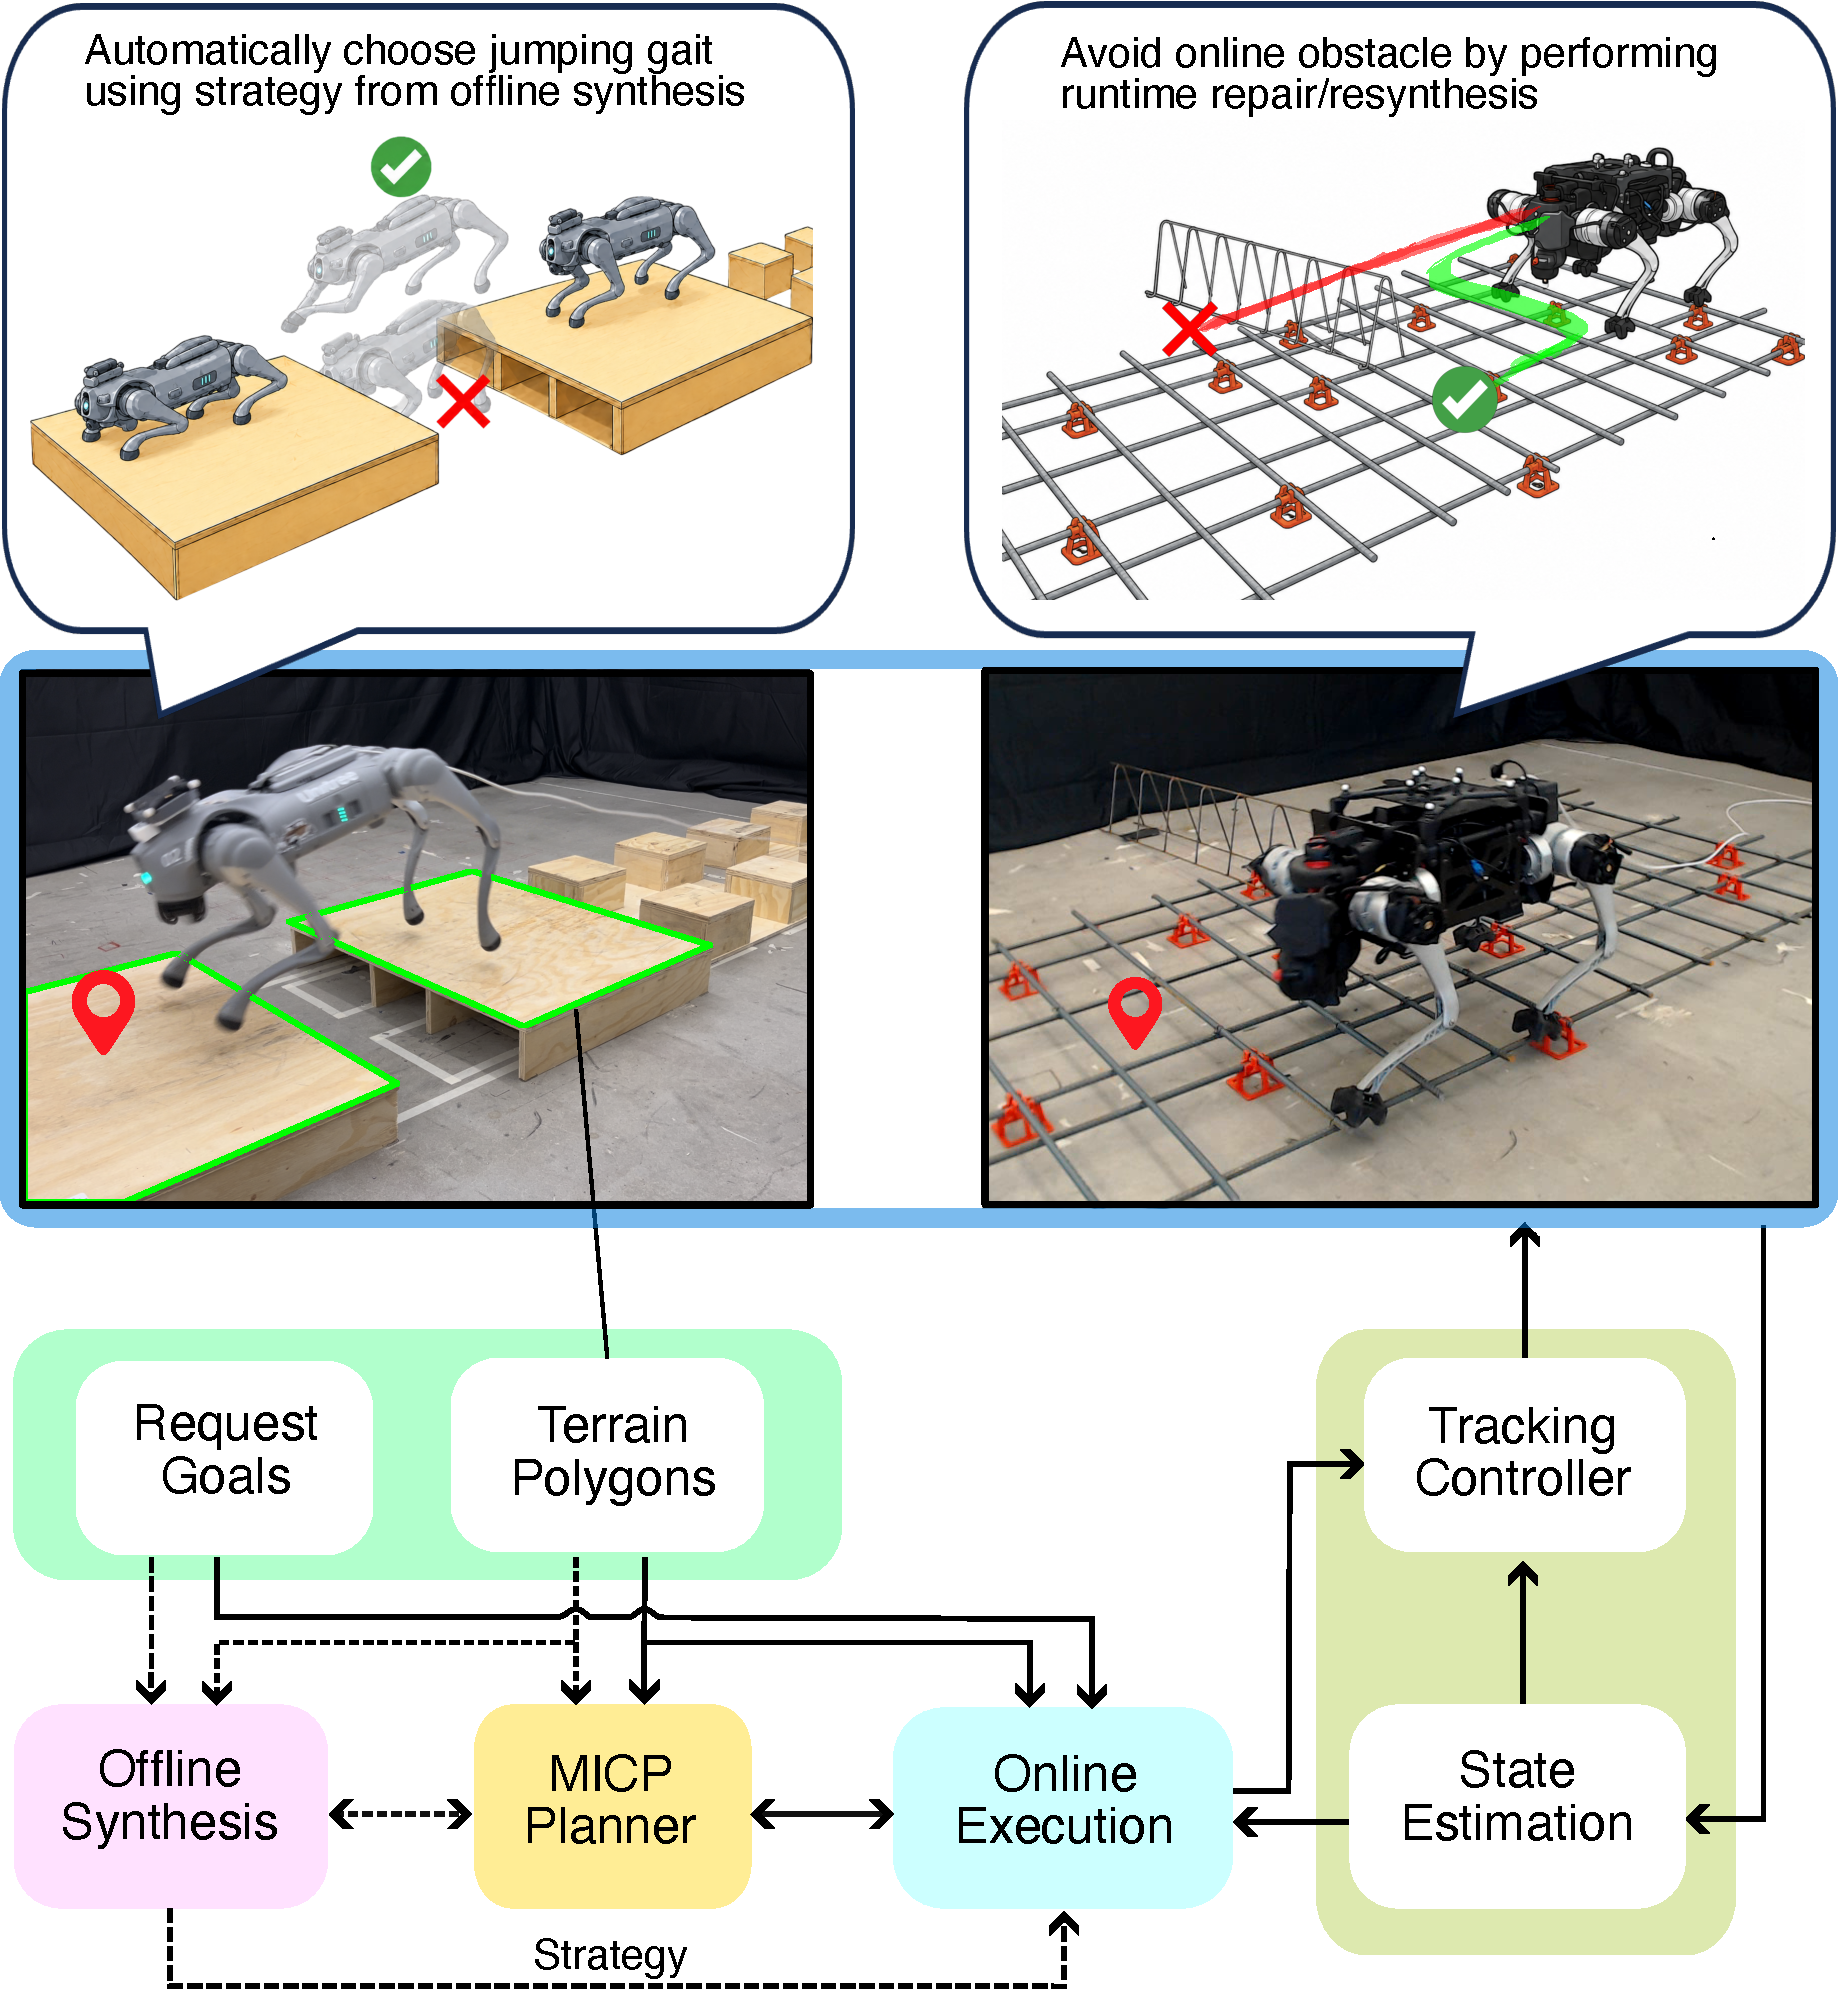
\includegraphics[width=1\linewidth]{system_diagram_v4.pdf}
    \caption{System architecture overview. The solid lines indicate online communication, while dashed lines represent offline processes.
    The request goals in the offline phase are user-defined, while those in the online phase are provided by a global planner based on the global goal.
    }
    \label{fig:system_diagram}
\end{figure}
%%%%%%%%%%%%%%%%%%%%%%%%%%%%%%%%%%%

Mixed-integer programming (MIP)-based methods \citep{valenzuela2016mixed,shirai2022simultaneous} model both contact state and contact surface selection for each leg and timestep as binary decision variables. This allows them to explicitly capture the interaction between terrain geometry and the robot's kinematic and dynamic constraints \citep{deits2014footstep}. When dynamics and constraints are suitably relaxed, the resulting convex approximation (MICP) provides a global certificate of feasibility upon convergence \citep{dai2019global}, making it a powerful tool for formally assessing locomotion viability.
However, the computational demands of MIP-based approaches scale poorly with increased terrain complexity and longer planning horizons, posing a major hurdle for real-time applications. To mitigate this, various simplifications have been proposed, such as fixing contact sequences \citep{ding2020kinodynamic,fey20243d}, constraining timing \citep{ponton2016convex,risbourg2022real,acosta2023bipedal}, or limiting the number of footsteps \citep{aceituno2017simultaneous}. Despite these efforts, scalability remains a challenge in cluttered environments with various terrain segments and features.

To simplify navigation across complex terrains, one effective strategy is to decompose long-horizon, global tasks into a sequence of localized, robot-centric environments centered around intermediate waypoints \citep{fankhauser2018robust}. Despite this simplification, the associated MIP formulation still faces computational challenges, as it must account for all nearby terrain elements.
To address this, we discretize the local environment and constrain each MIP to solving only a single discrete transition at a time. These discrete transitions are then composed using a Linear Temporal Logic (LTL)-based reactive synthesis framework \citep{bloem2012synthesis}, which enables us to systematically construct a correct-by-construction strategy that guides the robot through local decisions toward achieving its intermediate goals.
\revised{For readers unfamiliar with formal methods, LTL is a logic for expressing temporal properties of system behaviors using operators such as ``always,'' ``eventually,'' and ``until''~\citep{piterman2006synthesis,bloem2012synthesis}; reactive synthesis automatically constructs a controller (named as a \emph{strategy automaton} in this paper) that satisfies an LTL specification against any admissible environment behavior, providing correct-by-construction guarantees at the symbolic level.}

In this work, we present an integrated planning framework that unifies reactive synthesis with MIP-based optimization to enable legged robots to respond safely and efficiently to \revised{unforeseen terrain configurations revealed at runtime}. We abstract both the continuous robot states and local environmental context into symbolic representations, allowing the robot to make high-level decisions in real time for negotiating complex obstacles such as large gaps or cluttered terrain (see Fig.~\ref{fig:system_diagram}). Each symbolic transition is validated through an MICP to ensure the physical feasibility of the locomotion process. This architecture not only connects high-level symbolic reasoning with low-level dynamic feasibility, but also mitigates the computational challenges of solving long-horizon MICP problems.
By leveraging guidance from the LTL-based symbolic planner, each MICP instance only needs to handle short horizons and a limited set of terrain features, which substantially reduces computational load.
The framework is two-stage: in the offline synthesis stage, we employ \textit{gait-free} MICP formulations that jointly optimize over contact mode and foothold placement to precompute a diverse set of locomotion skills for symbolic transitions. During online deployment, we switch to lightweight \textit{gait-fixed} MICP formulations using these precomputed gaits, enabling real-time generation of physically consistent motions with real-world terrain data.

\revised{The two-stage architecture exposes two scalability challenges that we address with two complementary mechanisms. First, the full task specification has a state space that grows exponentially with the number of variables encoding the surrounding terrains, so direct synthesis is computationally impractical~\citep{bloem2012synthesis}; to address this, we propose a high-level manager that fixes the local terrain and goal information and only retains the skills needed for the current local environment, yielding an $80.9$--$90.1\%$ reduction in the symbolic variable count in our experiments. Second, gait-free MICP---used to certify dynamic feasibility---is itself computationally expensive; we therefore use a symbolic repair process that suggests only the missing transitions whose feasibility must be checked, yielding a $71.6$--$97.6\%$ reduction in costly gait-free MICP solves relative to exhaustive enumeration. During online execution, the gait-fixed MICP is re-solved against the actual perceived terrain to generate a new nominal trajectory, and runtime symbolic repair handles any unforeseen terrain that the offline phase did not cover.}

\revised{Closing the loop between this synthesis-MICP framework and a real robot poses two practical challenges that we address through two additional online-execution mechanisms. (i) Online MICP solve times are inherently variable, ranging from hundreds of milliseconds to several seconds, and can exceed the trajectory horizon used by the tracking controller. We propose a \emph{delay-aware coordination} scheme that asynchronously appends or stalls the tracking trajectory based on a formal two-case analysis of the per-transition timing budget; without it, the closed loop between the discrete strategy automaton and the continuous-time tracker is ill-defined under bounded solve time. (ii) The online MICP tends to become infeasible when the offline-checked target pose mismatches the actual terrain. We add a lightweight, zero-horizon \emph{kinematic-feasibility re-targeting} step that pre-checks and adjusts the desired pose at each transition, decoupling offline pose specification from online terrain geometry; the same online MICP is also augmented with additional collision-avoidance constraints for swing-foot clearance during a transition. Together with the offline scalability machinery, these mechanisms make the framework end-to-end deployable, which we validate on two robot hardware platforms and benchmark against both a pure-MIP planner and a heuristic foothold planner.}

The proposed framework remains flexible and modular---it can be driven by commands from a higher-level planner \citep{wermelinger2016navigation, fernbach2017kinodynamic,norby2020fast,chignoli2022rapid,liao2023walking,feng2023gpf} or directly from a user, and it easily accommodates new behaviors by expanding the symbolic transition set.

The main contributions of this work are summarized as follows:
\begin{itemize}
    \item \textbf{Integrated reactive-synthesis and MICP framework for terrain-adaptive locomotion.}
    Symbolic-level guidance limits the planning horizon and the number of terrain features any single MICP must consider, bridging high-level symbolic reasoning with low-level physical feasibility.

    \item \textbf{Scalable offline synthesis via a high-level manager and symbolic repair with dynamic feasibility checks.}
    The high-level manager reduces the symbolic state space by $80.9$--$90.1\%$, and symbolic repair, equipped with dynamic feasibility checks via gait-free MICP, generates only the necessary skills---reducing costly gait-free MICP solves by $71.6$--$97.6\%$ versus exhaustive enumeration.

    \item \textbf{Online execution module that bridges offline synthesis and real-world deployment.}
    The module re-solves a gait-fixed MICP against the actual perceived terrain at each symbolic transition, with \revised{delay-aware coordination between the strategy automaton and the tracking controller, online kinematic-feasibility re-targeting of the desired pose, and additional collision-avoidance constraints in the online MICP. Runtime symbolic repair handles previously unseen scenarios that were not considered offline.}

    \item \revised{\textbf{Comprehensive experimental validation.} We report simulation across four terrain scenarios with full per-module timing, comparisons against a pure MIP planner and a heuristic foothold planner, hardware deployment of the integrated stack on two robot platforms (Unitree Go2 and SkyMul Chotu), and a feasibility study of yaw orientation as a generalization case study.}
\end{itemize}

A conference version of this work is presented in \citep{zhou2025physically}. Beyond the conference paper, the current article contributes the delay-aware coordination and online re-targeting mechanisms motivated above, full hardware validation of the integrated framework on two robot platforms, systematic benchmarking against a pure-MIP planner and a heuristic foothold planner, a preliminary yaw-extension feasibility study, and substantially expanded preliminaries, related-work survey, and discussion of limitations.


% A conference version of this work is presented in \citep{zhou2025physically}. \revised{Following the IJRR convention for evolved-paper journal extensions, this article restates the framework introduced in the conference version and adds substantial new content. Beyond \citep{zhou2025physically}, the journal-specific contributions are: (i) kinematic-feasibility re-targeting of the robot's desired pose at each transition; (ii) delay-aware coordination between the strategy automaton and the tracking controller, with explicit two-case logic that handles MICP solve-time variability against the NMPC horizon; (iii) collision-region selection with binary variables and swing-foot clearance constraints in the MICP; (iv) full hardware deployment of the integrated stack on two robot platforms; (v) systematic benchmarking against a pure MIP planner and a heuristic foothold planner; (vi) a preliminary feasibility study of yaw orientation as a generalization direction; and (vii) expanded preliminaries, related-work survey, and discussion of limitations.}

%%%%%%%%% Related work %%%%%%%%
\section{Related Work}
\subsection{Hierarchical Planning for Terrain-Adaptive Locomotion}
Planning for terrain-adaptive locomotion can be boiled down into solving contact sequence and timing (equivalently gait), location (equivalently foothold), and robot motion (e.g., Center of Mass (CoM) or base pose), given the chosen kinematics/dynamics model and the perceived terrain information. Hierarchical approaches first separately or simultaneously address part of the above problems and then solve for the rest, which allows for higher computational efficiency.  
% Among them, hierarchical approaches commonly separate the foothold from the gait/contact and base pose planning, which allows for higher computational efficiency.
Kinematic footstep planning focuses on the first two problems, neglecting the robot dynamics through graph-based approaches \citep{kolter2008control,kalakrishnan2010fast,winkler2014path,mastalli2015line,fankhauser2018robust,griffin2019footstep} or optimization-based approaches \citep{deits2014footstep,tonneau2020sl1m,risbourg2022real, ren2025accelerating}.
% Another perspective of hierarchical approaches is on planning over a set of actions\citep{kolter2008control,kalakrishnan2010fast,winkler2014path,mastalli2015line,griffin2019footstep}.
Although non-fixed gait/contact plans can be generated for very rough terrains \citep{hauser2005non,bretl2006motion,tonneau2018efficient}, conservative quasi-static motions are generated for challenging terrains due to the kinematic simplification during  footstep planning. 
% While dynamically-feasible contact plans are also reported in, heavy computational time and difficulty in handling collision avoidance restrict the online re-planning.

Given the recent advances in optimization-based approaches, notably Model Predictive Control (MPC), another focus of the literature is on the local foothold adaptation and the integration of robot dynamics for dynamic locomotion.
Instantaneous foothold adaptation around a nominal location, with a fixed and cyclic gait, is performed based on heuristic search \citep{jenelten2020perceptive,kim2020vision,agrawal2022vision} or learning approaches \citep{magana2019fast, villarreal2020mpc,yu2021visual,gangapurwala2022rloc, wu2025learn, Kamohara2025RLMPC}. 
In \citep{grandia2021multi,jenelten2022tamols,grandia2023perceptive}, the base pose and foothold are optimized jointly, demonstrating impressive terrain traversing capabilities on rough terrains. More recently, MPC has been employed within hierarchically integrated planning frameworks for legged navigation over rough terrain, incorporating explicit terrain uncertainty quantification \citep{muenprasitivej2024bipedal, shamsah2025terrain, muenprasitivej2026bipedal}.
% , which generates dynamically consistent trajectories. 

However, the above dynamic locomotion works consider a fixed gait pattern that usually prohibits achieving versatile behaviors, such as jumping.
In \citep{Park2015OnlinePF, kim2020vision,gilroy2021autonomous}, jumping motions are generated offline and triggered through heuristics.
In \citep{fernbach2017kinodynamic,norby2020fast,chignoli2022rapid}, RRT-Connect is used for rapid kino-dynamic locomotion planning, and the switch between normal walking and jumping is either embedded inside a reduced-order model during sampling \citep{norby2020fast} or decided by a pre-trained feasibility classifier \citep{chignoli2022rapid}.
Beyond limited gait modes, other works focus on online gait planning and/or foothold selection and deploy MPC to track the plan,
which can be further categorized into model-free \citep{da2021learning,yang2022fast,xie2022glide,pmlr-v164-margolis22a,yu2024learning} and model-based methods \citep{boussema2019online,wang2023and,sun2023free}.

\revised{A complementary line of work uses end-to-end reinforcement learning (RL) to train perceptive locomotion policies that directly map terrain observations to joint commands, achieving impressive robustness on stairs, gaps, and unstructured outdoor terrain~\citep{miki2022learning,agarwal2023legged,zhuang2023robot,hoeller2023anymal,cheng2024extreme,luo2024pie}. Compared with these data-driven approaches, our model-based, formal-methods framework offers explicit symbolic-level realizability guarantees and physical-feasibility certificates from MICP, at the cost of weaker generalization and the need for a terrain abstraction; we view the RL approaches and ours as complementary rather than competing.}

\subsection{Simultaneous Planning via Optimization}
Planning for terrain-adaptive locomotion problem can also be formulated as a combinatorial optimization problem that simultaneously optimizes for gait, foothold, and robot dynamics.
One approach is to incorporate rigid \citep{posa2014direct} or smoothed \citep{mordatch2012discovery, drnach2021robust} complementarity constraints, which accurately model the physical contact interaction behavior but remains computationally inefficient due to the non-smoothness and high nonlinearity. Promising online contact-implicit MPC results are reported in \citep{aydinoglu2022real,le2024fast, drnach2022mediating} but still limited to low-dimensional system or static environment. 

Another way of encoding discrete contact decisions is to treat both the contact state and the contact plane selection for each leg at each timestep as binary variables \citep{valenzuela2016mixed,shirai2022simultaneous,jiang2023locomotion}. The underlying problem can be formulated as Mixed Integer Program (MIP). Convex approximations of nonlinear dynamics, usually centroidal dynamics, and constraints are typically required to transform the MIP into a more tractable Mixed Integer Convex Program (MICP), albeit with an increased number of binary variables. 
A global certificate for the approximated convex problem exists upon convergence \citep{dai2019global}, providing an ideal means to determine the feasibility in our proposed method.
To relieve the computational burden due to the introduction of many binary variables, the works of \citep{ponton2016convex,ding2020kinodynamic,acosta2023bipedal} assume the contact sequence and timing are chosen \textit{a priori}, and only optimize the contact plane selection. Aceituno-Cabezas et al. \citep{aceituno2017simultaneous} optimize the contact sequence within a certain gait cycle that fixes the number of footsteps. 
However, it is inevitable that the problem complexity grows exponentially when the number of discrete contact options increases along with the time horizon and terrain features. Our work aims to alleviate computational burden through a two-stage approach. In the offline phase, expensive MICPs that optimize both contact state and foothold selection are solved to generate necessary locomotion gaits. In the online phase, efficient MICPs with adaptive and predefined gaits are used to produce dynamically feasible motions and footholds. Additionally, guided by a synthesis-based task planner, each MICP in our work considers shorter time horizons and fewer terrain features compared to solving a single large MICP problem.

% Our approach: between hierarchical planning and combinatorial optimization. Split the contact planning problem into gait and footstep selections, while the gait planner considers dynamical feasibility given the terrain information.

% Different from \citep{shirai2022simultaneous}, this work: 

% 1. Considers the angular evolvement of the robot to allow more versatile motion generation 

% 2. We consider a more complicated centroidal optimization problem which provides higher-fidelity solution back to the MICP 

% 3. We fix the gait selection to allow real-time foothold selection 

 

% Different from the LGP work \citep{toussaint2015logic}: 

% 1. We evaluate the entire course of a trajectory and incorporate the underactuated dynamics, which is hard to be divided into multiple sub-problems. 

% Different from the MCTS \citep{amatucci2022monte}: 

% 1. We mostly care about the computational efficiency and the motion feasibility across a certain course. Therefore, two different choices we made here: 

% 2. Our footstep planner assumes a fixed gait and only determines the foothold locations given the steppable regions. 

% 3. The gait selection in our problem setup stays in a relatively higher level, whereas the MCTS is able to discover and optimize the gait. In other words, the high-level search space in our framework is smaller than MCTS.   

% Independent Gait Scheduling

% As discussed above, simultaneously planning for the gait and the footholds given perception feedback remains a challenging problem. Alternatively, impressive results have been reported by separating the gait scheduling and the foothold selection. The state-of-the-art works that handle gait transitions can be divided into model-free \citep{da2021learning,yang2022fast,xie2022glide,pmlr-v164-margolis22a}... and model-based approaches \citep{boussema2019online,wang2023and,sun2023free}.

\subsection{Task and Motion Planning for Contact-Rich Planning}
% Instead of capturing every discrete option as in general MIP, 
Task and Motion Planning (TAMP) formally defines symbolic-level tasks and searches through a graph of predefined motion primitives that enable feasible symbolic transitions \citep{garrett2021integrated, zhao2024survey}. For more complex physical contact resoning, Toussaint et al. propose Logic Geometric Programming (LGP) \citep{toussaint2015logic} and embed the high-level
logic representation into the low-level motion planner, demonstrating contact-rich tool-use behaviors \citep{toussaint2018differentiable}
after defining abundant action primitives. 
Building on this, a broader range of motions has been showcased, including versatile manipulation \citep{migimatsu2020object,zhao2021sydebo} and loco-manipulation tasks \citep{sleiman2023versatile}.
In a similar vein, works such as \citep{ding2021hybrid,shirai2021lto,jelavic2021combined,amatucci2022monte,chen2021trajectotree,zhang2023simultaneous,zhu2023efficient,asselmeier2024hierarchical} integrate graph-search or sampling-based methods with optimization-based approaches in a holistic manner, abstracting contact modes within a discrete domain. However, the combinatorial nature of these problems often leads to poor scalability due to the explosion of contact modes. Deploying such approaches online in dynamic environments remains an open challenge. From a different perspective, we abstract a smaller set of task-level contact modes as locomotion gaits over a specific time horizon and distance, allowing the MICP to solve for details such as contact locations and robot motion during execution. This shifts the focus to selecting locomotion gaits within a local environment while ensuring safety and completeness through synthesis-based approaches.

Unlike LGP that solves an integrated TAMP problem, synthesis-based approaches using Linear Temporal Logic (LTL) operate primarily at the task level, emphasizing safety and completeness guarantees within the task domain \citep{kress2018synthesis}. These methods typically synthesize a sequence of task-level actions, which are then executed by a motion planner. Recently, LTL has been applied to safe locomotion tasks, employing distinct task-level abstractions on topological maps of terrain \citep{kulgod2020temporal,zhou2022reactive,jiang2023abstraction} or locomotion keyframes for reduced-order models \citep{gu2022reactive,shamsah2023integrated,zhao2022reactive}.
Reactive synthesis \citep{pnueli1989synthesis}, widely applied to mobile robots \citep{kress2009temporal}, has been employed to enable prompt decision-making in response to more complex environments \citep{shamsah2023integrated} or external perturbations \citep{gu2022reactive}. Notably, \citep{zhao2022reactive} formulate the terrain-adaptive locomotion problem as a sequential decision-making task, selecting appropriate locomotion modes with predefined contact and locomotion keyframes to accommodate dynamically changing terrains. However, the locomotion mode selection is explicitly encoded in the LTL specification using expert knowledge, lacking a physically feasibility guarantee.
% To reduce the complexity of solving multi-contact, long-horizon, and kino-dynamic planning problems, a single optimization problem can be divided into multiple sub-problems, facilitating faster computation through holistic approaches. Graph-search planning (GSP) or sampling-based planning (SBP) methods have been proposed to be combined with dynamically feasible motion primitives \citep{shkolnik2011bounding, fernbach2017kinodynamic,norby2020fast,shirai2021lto,ding2021hybrid,jelavic2021combined,chignoli2022rapid,amatucci2022monte}. Superior planning speed has been reported with reduced-order models \citep{fernbach2017kinodynamic,norby2020fast,carpentier2018multicontact} or pre-trained feasibility classifier \citep{chignoli2022rapid}. 
% The authors in \citep{zhao2021sydebo,shirai2021lto,ding2021hybrid,jelavic2021combined,amatucci2022monte,chen2021trajectotree,zhang2023simultaneous} fully exploit the robot dynamics through TO combined with a high-level search. 
% Among them, researchers in \citep{jelavic2021combined,amatucci2022monte} explicitly reason the gait/contact mode in the search process. 
% However, the combinatorial nature of the problem renders poor scalability due to the explosion of contact modes. Online deployment of this type of approaches given changing terrain information remains an open problem.
In this work, we aim to combine the strengths of reactive synthesis and MICP, utilizing the global certificate of MICP as a feasibility checker for terrain-adaptive locomotion.

% The lack of immediate reaction and safety guarantee given real-time terrain information still prohibits this type of approach from online deployment.

\subsection{Physically-Feasible Reactive Synthesis}
% Linear Temporal Logic (LTL) serves as a prevalent tool for encoding temporal task specifications and automating the synthesis of system transition behaviors within the robotics community. Originating from its proposal for model checking by Pnueli in 1977 \citep{pnueli1977temporal}, LTL has gained substantial traction in robotics research, initially prevalent in studies involving wheeled robots \citep{kress2009temporal, decastro2018collision}, and more recently, extending to legged robots \citep{warnke2020towards, zhao2022reactive, kulgod2020temporal, gu2022reactive, shamsah2023integrated}.
% Reactive Synthesis, denoting the automated generation of a reactive system to ensure compliance with desired specifications, regardless of external inputs, was introduced by Pnueli in 1989 \citep{pnueli1989synthesis}. Given the escalating complexity associated with lengthy LTL formulas, a subset of LTL, General Reactivity of Rank 1 (GR(1)), was proposed to streamline the synthesis process \citep{piterman2006synthesis}. This subset proves especially beneficial in managing the synthesis process efficiently.

% (Replanning in the task level; BT, TAMP; inflation? Check Jonas paper again) 

% In contrast to Task and Motion Planning (TAMP), a paradigm that typically integrates symbolic search with geometric or optimization-based motion planners, reactive synthesis primarily operates at the task level. 

% Reactive synthesis primarily operates at the task level and involves specifying Linear Temporal Logic (LTL) formulas that encompass sequencing, conditions, and reactions to environmental events. 
While reactive synthesis can promptly and safely respond to dynamic environments, it typically does not assess physical feasibility when being deployed on complex robotic systems. To bridge the gap between discrete abstraction and continuous system dynamics, various strategies have been proposed. Studies in  \citep{decastro2014dynamics,fainekos2006translating} focus on automatically synthesizing controllers in the continuous domain based on high-level specifications. Another approach involves incorporating dynamics directly into the reactive synthesis process by abstracting physical systems, including nonlinear \citep{bhatia2010sampling}, switched \citep{liu2013synthesis}, and hybrid systems \citep{maly2013iterative} with manageable model complexity. However, for legged robots with multiple contacts navigating dynamic terrains, these physically feasible reactive synthesis approaches remain computationally intractable.

Recent efforts \citep{pacheck2020finding, pacheck2022physically} focus on symbolic repair for unrealizable task specifications, defining symbolic skills with preconditions and postconditions, similar to TAMP, to identify missing skills that make the specification realizable. These works introduce iterative feasibility checks based on symbolic repair suggestions, emphasizing alignment between symbolic task specifications and physical reality. Building upon this, Meng et al. \citep{meng2024automated} extend this type of approach to online symbolic repair.
Inspired by these works, Zhou et al. \citep{zhou2025physically} adopt a similar mechanism for terrain-adaptive locomotion. Specifically, they abstract the robot and terrain states in a local environment and define physically feasible skills by solving MICP. 
% To address scalability issues arising from complex terrain features, they employ a high-level manager to decompose the problem into smaller subproblems, enabling faster repair and synthesis. 
They leverage high-level manager and symbolic repair to efficiently identify missing but necessary skills, reducing the need for frequent calls to the computationally expensive gait-free MICP. Our work significantly completes \citep{zhou2025physically} through seamless integration with a low-level tracking control module, enabling systematic benchmarking, and demonstrating real-world hardware deployment.

% Three main novelties in our reactive planner:

% 1) We leverage the powerfulness of reactive synthesis to  reason about the robot traversability with regard to the terrain information.

% 2) We generate skills that are physically feasible offline; a symbolic repair process is proposed to handle unrealizable specifications.

% 3) We perform fast run-time feasibility checking through graceful coordination toward MPC given real-time robot and environment representations.

%%%%%%%%% Preliminaries %%%%%%%%
\section{Preliminaries}
Consider a robot equipped with sensors navigating an environment toward a designated global goal $g_{\textrm{global}} \in \mathbb{R}^2$. This task can be broken into a sequence of local navigation subtasks, where the robot moves toward intermediate local request goals $\mathcal{G}_{\textrm{local}}$, determined by a global planner based on the nearby segmented terrain polygons $\mathcal{P}$. We illustrate an instance of such a local task setup.
% following the same example introduced in \citep{zhou2025physically}.
% throughout the paper.

\noindent
\textbf{Example~\examplelabel{example:1}}.
% (9-grid locomotion). 
\textit{
Consider a 2D grid world with nine cells (in yellow) in Fig.~\ref{fig:preliminary_nine_squares}. The robot is required to move from an initial cell (e.g. the center cell) 
to a desired goal cell indicated by the star. 
Each cell is assigned a terrain type, such as $\textit{Dense}$ or $\textit{Sparse}$ stepping stones.}

%%%%% Fig. 9 grid %%%%
\begin{figure}[ht]
    \centering
    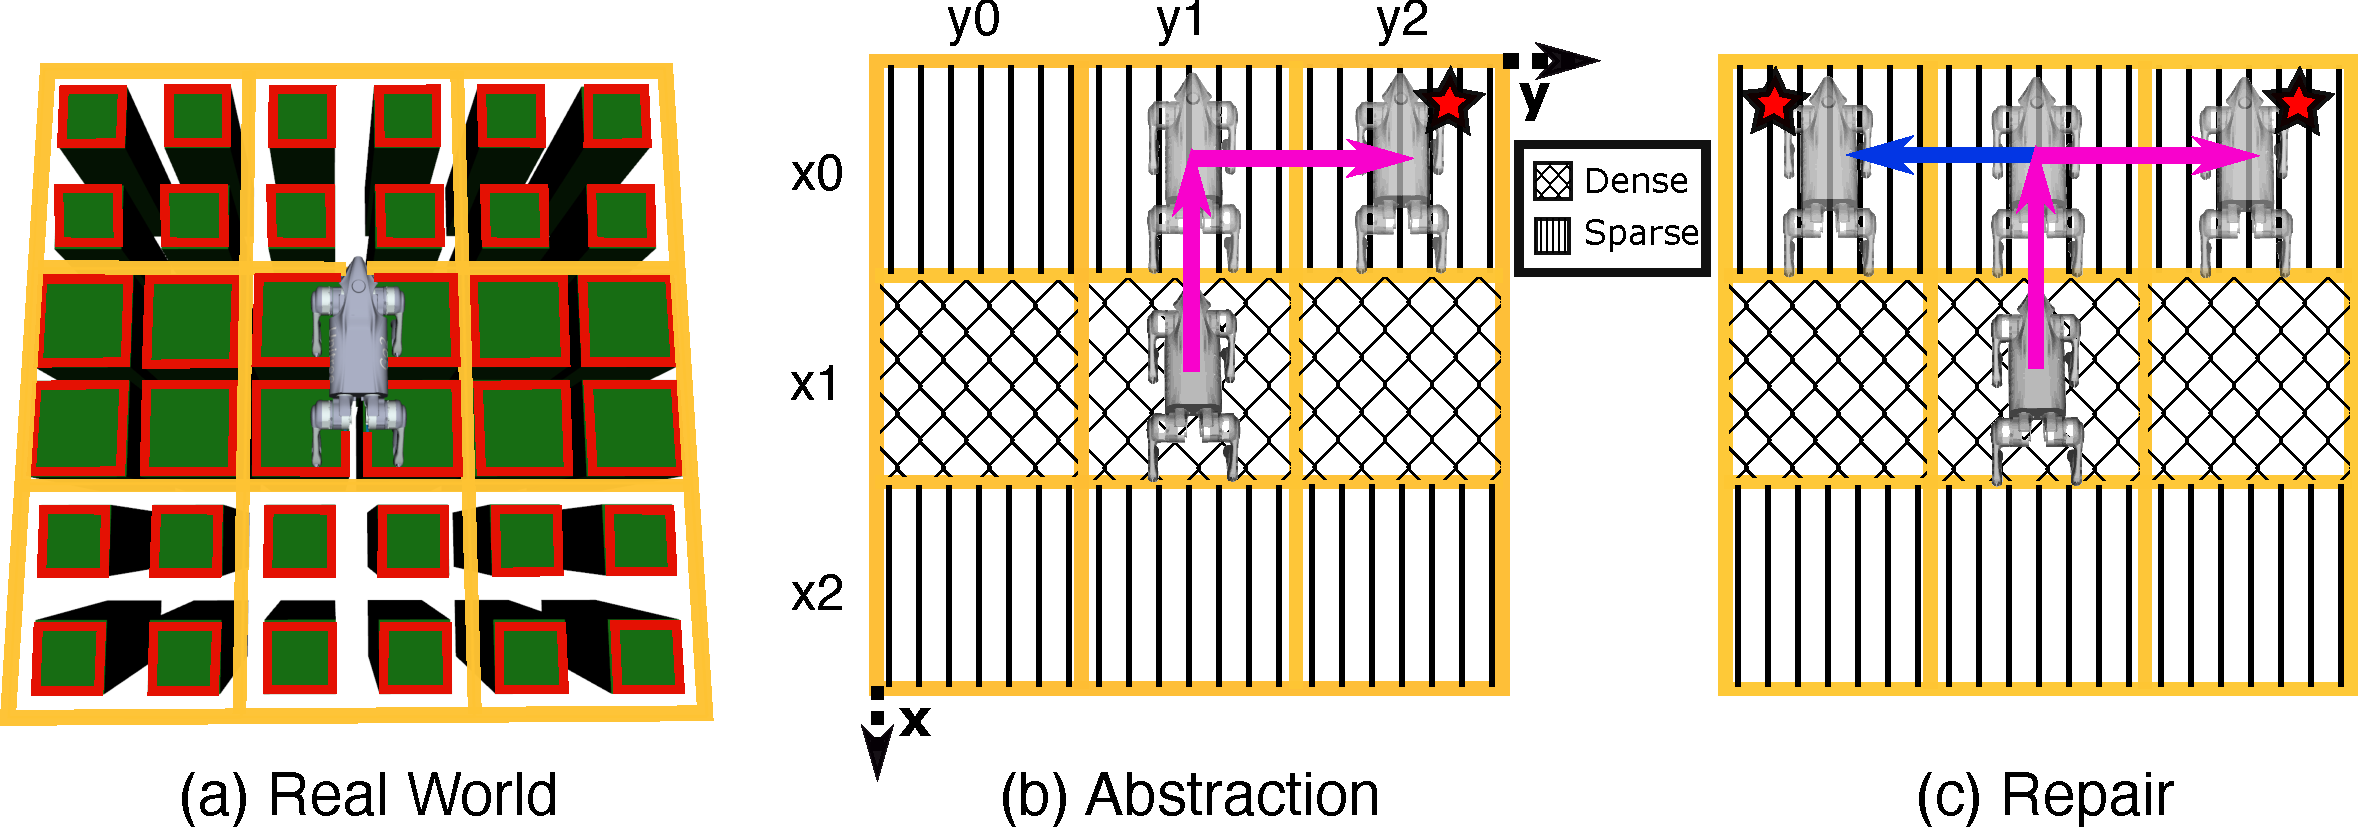
\includegraphics[width=\linewidth]{preliminary_drawing.pdf}
    \caption{Terrain abstraction and skill definition. (a) Top-down view of the real-world terrain before abstraction. The red polygons denote the segmented terrain polygons. (b) Abstraction of the terrain and robot's skills (pink) moving from one location to another. (c) Repair process to find a new skill (blue).}
    \label{fig:preliminary_nine_squares}
\end{figure}
%%%%%%%%%%%%%%%

\subsection{Abstractions}\label{sec:preliminaries_abstraction}

% Given a set of terrain polygons $\mathcal{P}$,
% e.g.,
% in Fig.~\ref{fig:preliminary_nine_squares}(a),
% we abstract them into a 2D grid of size $n\times m$.
% For each dimension,
% we denote each location in that dimension with a symbol,
% resulting in two sets
% $\xcells \coloneqq \{x_0, \dots, x_{n-1}\}$
% and
% $\ycells \coloneqq \{y_0, \dots, y_{m-1}\}$.
% %
% We define a set of atomic propositions 
% $\ap$,
% partitioned
% into sets of inputs $\mathcal{I}$
% and outputs $\mathcal{O}$,
% to describe the symbolic world states and robot actions.
% The inputs $\mathcal{I}$ consist of
% the robot inputs 
% $\inpcen$,
% the request inputs 
% $\inprequest$,
% and
% the terrain inputs $\inpterrain$
% ($\inp = \inpcen \cup \inprequest \cup \inpterrain$).
% The robot inputs 
% $\inpcen \coloneqq 
% \{\var_x \mid x \in \xcells\} \cup 
% \{\var_y \mid y \in \ycells\}$
% are used to abstract the robot position,
% the request inputs
% $\inprequest \coloneqq
% \{\var_x^\textrm{req} \mid x \in \xcells\} \cup 
% \{\var_y^\textrm{req} \mid y \in \ycells\}
% $
% are used to abstract the requested goal cells,
% and
% the terrain inputs
% $\inpterrain \coloneqq \{
% \tvar{x}{y} \mid x\in \xcells, y\in \ycells
% \}$
% describe 
% the terrain type of the grid cells.
% %
% The robot state can be extended to incorporate orientation information, such as the floating base's yaw angle, as demonstrated in Sec.~\ref{sec:extension}.
% We then consider a finite set of size $n_t$ of terrain types, 
% defined based on their physical characteristics. 
% For $\physicalstate \in \naturals$, we denote $\range{\physicalstate} \coloneqq \{0, \dots, \physicalstate - 1\}$.
% We note that 
% terrain inputs $\tvar{x}{y} \in \inpterrain$
% are integer variables
% belonging to $\range{n_t}$,
% and we translate them into a set of Boolean propositions,
% as done in~\citep{ehlers2016slugs}.
% %
% An input state 
% $\inpstate$
% is 
% a value assignment function
% $\inpstate: \inp \to \{\true, \false\} \cup \range{n_t}$. Since the robot can only be in one cell at a time, and the goal is a single cell, we require that exactly one $\var_x$, one $\var_y$, one $\var_x^\textrm{req}$, and one $\var_y^\textrm{req}$ be $\true$, for each input state. 
% The robot states $\inpstatecen: \inpcen \to \{\true, \false\}$,
% request states
% $\inpstaterequest: \inprequest \to \{\true, \false\}$,
% and
% terrain states
% $\inpstateterrain: \inpterrain \to \range{n_t}$
% are the projections of $\inpstate$ on 
% $\inpcen$,
% $\inprequest$,
% and $\inpterrain$, respectively.
% We denote the sets of input states as $\inpstates$,
% robot states as $\inpstatescen$,
% request states as $\inpstatesrequest$,
% and 
% terrain states as $\inpstatesterrain$.

Given a set of terrain polygons $\mathcal{P}$, such as those in Fig.~\ref{fig:preliminary_nine_squares}(a), we abstract them into a 2D grid of dimension $n \times m$. For each axis, we label every position with a symbol, producing two sets: $\xcells \coloneqq \{x_0, \dots, x_{n-1}\}$ and $\ycells \coloneqq \{y_0, \dots, y_{m-1}\}$.

We introduce a collection of atomic propositions $\ap$, partitioned into input variables $\mathcal{I}$ and output variables $\mathcal{O}$, which capture the symbolic world state and robot actions. The inputs $\mathcal{I}$ include robot position inputs $\inpcen$, request inputs $\inprequest$, and terrain inputs $\inpterrain$, with $\inp = \inpcen \cup \inprequest \cup \inpterrain$.
The robot inputs are defined as $\inpcen \coloneqq \{\var_x \mid x \in \xcells\} \cup \{\var_y \mid y \in \ycells\}$ to represent the robot’s location. Request inputs are given by $\inprequest \coloneqq \{\var_x^\textrm{req} \mid x \in \xcells\} \cup \{\var_y^\textrm{req} \mid y \in \ycells\}$ to represent the desired goal cell. The terrain inputs are defined as $\inpterrain \coloneqq \{\tvar{x}{y} \mid x \in \xcells, y \in \ycells\}$, which describe the terrain type associated with each grid cell.
We assume a finite set of terrain types of size $n_t$, defined according to their physical characteristics. For $\physicalstate \in \naturals$, we denote $\range{\physicalstate} \coloneqq \{0, \dots, \physicalstate - 1\}$. Accordingly, each terrain input $\tvar{x}{y} \in \inpterrain$ is an integer variable taking values from $\range{n_t}$, which we further translate into Boolean propositions following the approach of~\citep{ehlers2016slugs}. The robot state abstraction can also be extended to incorporate orientation, such as the yaw angle of the floating base (see Sec.~\ref{sec:extension}).

An input state $\inpstate$ is a mapping $\inpstate: \inp \to \{\true, \false\} \cup \range{n_t}$. Because the robot and its goal occupy only a single grid cell each, exactly one $\var_x$, one $\var_y$, one $\var_x^\textrm{req}$, and one $\var_y^\textrm{req}$ must evaluate to $\true$ for any valid input state. We denote projections of $\inpstate$ as robot states $\inpstatecen: \inpcen \to \{\true, \false\}$, request states $\inpstaterequest: \inprequest \to \{\true, \false\}$, and terrain states $\inpstateterrain: \inpterrain \to \range{n_t}$. The complete sets of such states are denoted by $\inpstates$, $\inpstatescen$, $\inpstatesrequest$, and $\inpstatesterrain$, respectively.

% We use a grounding function to describe the physical meaning of 
% input states.
% Consider
% a physical state space $\ps \subseteq \reals^n$
% that represents the physical world, including the 
% robot's position, orientation, and terrain properties.
% The grounding function
% $\grounding: \inpstates \to 2^\ps$
% maps each input state $\inpstate$ to a set of physical states in $\ps$.
% For robot states
% $\inpstatecen \in \inpstatescen$,
% we define 
% $\grounding(\inpstatecen) \coloneqq \{
% \physicalstate \in \ps \mid
% \exists \var_x, \var_y \in \inpcen. 
% \inpstatecen(\var_x) \land \inpstatecen(\var_y) \land
% \textrm{robot\_pose}(\physicalstate) \in \textrm{cell}(x,y)
% \}$.
% Similarly, for request states 
% $\inpstaterequest \in \inpstatesrequest$,
% we define
% $\grounding(\inpstaterequest) \coloneqq \{
% \physicalstate \in \ps \mid
% \exists \var_x^\textrm{req}, \var_y^\textrm{req} \in \inprequest. 
% \inpstaterequest(\var_x^\textrm{req}) \land \inpstaterequest(\var_y^\textrm{req}) \land
% \textrm{request\_goal}(\physicalstate) \in \textrm{cell}(x,y)
% \}$.
% For terrain states $\inpstateterrain \in \inpstatesterrain$,
% we define
% $\grounding(\inpstateterrain)$
% to be the set of physical states
% whose abstracted terrain types are indicated by $\inpstateterrain$.
% For an input state $\inpstate \in\inpstates$ whose
% projections are $\inpstatecen$, $\inpstaterequest$, and $\inpstateterrain$,
% $\grounding(\inpstate) \coloneqq \grounding(\inpstatecen) \cap \grounding(\inpstaterequest) \cap \grounding(\inpstateterrain)$.
% Lastly,
% we use an inverse grounding function 
% $\inversegrounding: \ps \to \inpstates$
% to map a physical state $\physicalstate \in \ps$
% to its corresponding input state.

We introduce a grounding function to associate symbolic input states with their physical interpretations. Let the physical state space be $\ps \subseteq \reals^n$, which encodes the physical world, including the robot’s position, orientation, and terrain attributes. The grounding function $\grounding: \inpstates \to 2^\ps$ maps each input state $\inpstate$ to the corresponding set of physical states in $\ps$.

For robot states $\inpstatecen \in \inpstatescen$, we define 
$\grounding(\inpstatecen) \coloneqq \{
\physicalstate \in \ps \mid
\exists \var_x, \var_y \in \inpcen. 
\inpstatecen(\var_x) \land \inpstatecen(\var_y) \land
\textrm{robot\_pose}(\physicalstate) \in \textrm{cell}(x,y)
\}$.
Similarly, for request states $\inpstaterequest \in \inpstatesrequest$, we set
$\grounding(\inpstaterequest) \coloneqq \{
\physicalstate \in \ps \mid
\exists \var_x^\textrm{req}, \var_y^\textrm{req} \in \inprequest. 
\inpstaterequest(\var_x^\textrm{req}) \land \inpstaterequest(\var_y^\textrm{req}) \land
\textrm{request\_goal}(\physicalstate) \in \textrm{cell}(x,y)
\}$. 
For terrain states $\inpstateterrain \in \inpstatesterrain$, the grounding $\grounding(\inpstateterrain)$ is defined as the set of physical states whose terrain abstractions are consistent with $\inpstateterrain$.
Given an input state $\inpstate \in \inpstates$ with projections $\inpstatecen$, $\inpstaterequest$, and $\inpstateterrain$, we combine them as
$\grounding(\inpstate) \coloneqq \grounding(\inpstatecen) \cap \grounding(\inpstaterequest) \cap \grounding(\inpstateterrain)$.
Finally, we introduce an inverse grounding function $\inversegrounding: \ps \to \inpstates$ that maps each physical state $\physicalstate \in \ps$ back to its corresponding symbolic input state.

% In Example~\ref{example:1},
% the inputs are
% $\inpcen \coloneqq 
% \{
% \var_{x_0}, \var_{x_1}, \var_{x_2},
% \var_{y_0}, \var_{y_1}, \var_{y_2}
% \}$,
% $\inprequest \coloneqq \{\var^\textrm{req} \mid \var \in \inpcen\}$,
% and
% $\inpterrain \coloneqq \{\tvar{x_i}{y_j} \mid i,j\in 
% \{0,1,2\}
% \}$
% where 
% $\tvar{x_i}{y_j} = 1$ if the terrain type of the grid cell $(x_i, y_j)$ is Dense,
% and $\tvar{x_i}{y_j} = 0$ if it is Sparse.
% The input state in Fig.~\ref{fig:preliminary_nine_squares}(b) is
% $\inpstate: 
% \var_{x_1} \mapsto \true, 
% \var_{y_1} \mapsto \true,
% \var_{x_0}^\textrm{req} \mapsto \true, 
% \var_{y_2}^\textrm{req} \mapsto \true,
% \tvar{x_1}{y_j} \mapsto 1$ for $j\in\{0,1,2\}$.
% In this paper,
% we omit the Boolean propositions that are $\false$ and integer propositions
% whose values are $0$ in the input states for space.

In Example~\ref{example:1}, the inputs are defined as
$\inpcen \coloneqq
\{
\var_{x_0}, \var_{x_1}, \var_{x_2},
\var_{y_0}, \var_{y_1}, \var_{y_2}
\}$,
$\inprequest \coloneqq \{\var^\textrm{req} \mid \var \in \inpcen\}$,
and
$\inpterrain \coloneqq \{\tvar{x_i}{y_j} \mid i,j\in {0,1,2}\}$,
where $\tvar{x_i}{y_j} = 1$ if the grid cell $(x_i, y_j)$ is classified as Dense, and $\tvar{x_i}{y_j} = 0$ if it is Sparse.
The input state shown in Fig.~\ref{fig:preliminary_nine_squares}(b) is
$\inpstate:
\var_{x_1} \mapsto \true,
\var_{y_1} \mapsto \true,
\var_{x_0}^\textrm{req} \mapsto \true,
\var_{y_2}^\textrm{req} \mapsto \true,
\tvar{x_1}{y_j} \mapsto 1 \ \text{for } j\in \{0,1,2\}$.
For brevity, throughout this paper we omit Boolean propositions set to $\false$ and integer propositions with value $0$ when describing input states.

% The aforementioned output propositions 
% $\out$ 
% represent
% the skills 
% that allow the robot to transit among grid cells,
% given their corresponding terrain states.
% A skill $\skill \in \out$
% consists of 
% sets of preconditions $\skillpre \subseteq \inpstatescen \times \inpstatesterrain$,
% from which the skill is allowed to execute,
% and 
% postconditions $\skillpost \subseteq \inpstatescen$, the resulting grid cell after executing the skill.
% In Example~\ref{example:1},
% the skill $\skillcustom{0}$ moves the robot from the middle to the upper terrain grid cell (Fig.~\ref{fig:preliminary_nine_squares}b).
% The precondition of $\skillcustom{0}$ is
% $\skillprecustom{\skillcustom{0}} = \{
% (\inpstatecen, \inpstateterrain): \var_{x_1}\mapsto \true, 
% \var_{y_1} \mapsto \true,
% \tvar{x_1}{y_0} \mapsto 1, 
% \tvar{x_1}{y_1} \mapsto 1, 
% \tvar{x_1}{y_2} \mapsto 1
% \}$, 
% The postcondition is
% $\skillpostcustom{\skillcustom{0}} = \{
% \inpstatecen:
% \var_{x_0} \mapsto \true, 
% \var_{y_1} \mapsto \true
% \}$.
% In addition,
% each skill consists of
% a continuous-level locomotion gait, 
% e.g. a one-second trotting gait $L$,
% that physically implements the symbolic transition
% (Sec.~\ref{sec:motion_primitive}).

The output propositions
$\out$
represent skills that enable the robot to move between grid cells under specific terrain conditions.
A skill $\skill \in \out$ is defined by its preconditions
$\skillpre \subseteq \inpstatescen \times \inpstatesterrain$,
which specify the robot and terrain states from which it can be executed,
and its postconditions
$\skillpost \subseteq \inpstatescen$,
which describe the resulting robot state after execution.
In Example~\ref{example:1}, the skill $\skillcustom{0}$ moves the robot from the middle cell to the upper cell (Fig.~\ref{fig:preliminary_nine_squares}b).
The precondition of $\skillcustom{0}$ is
$\skillprecustom{\skillcustom{0}} = \{ (\inpstatecen, \inpstateterrain): \var_{x_1}\mapsto \true, \var_{y_1}\mapsto \true, \tvar{x_1}{y_0}\mapsto 1, \tvar{x_1}{y_1}\mapsto 1, \tvar{x_1}{y_2}\mapsto 1 \}$,
while the postcondition is
$\skillpostcustom{\skillcustom{0}} = \{ \inpstatecen: \var_{x_0}\mapsto \true, \var_{y_1}\mapsto \true \}$.
Each symbolic skill is also paired with a continuous-level locomotion gait, such as a one-second trotting gait $L$, which physically realizes the symbolic transition (Sec.~\ref{sec:motion_primitive}).

%%%% Fig.2 System architecture %%%%
% \begin{figure}[t]
%     \centering
%     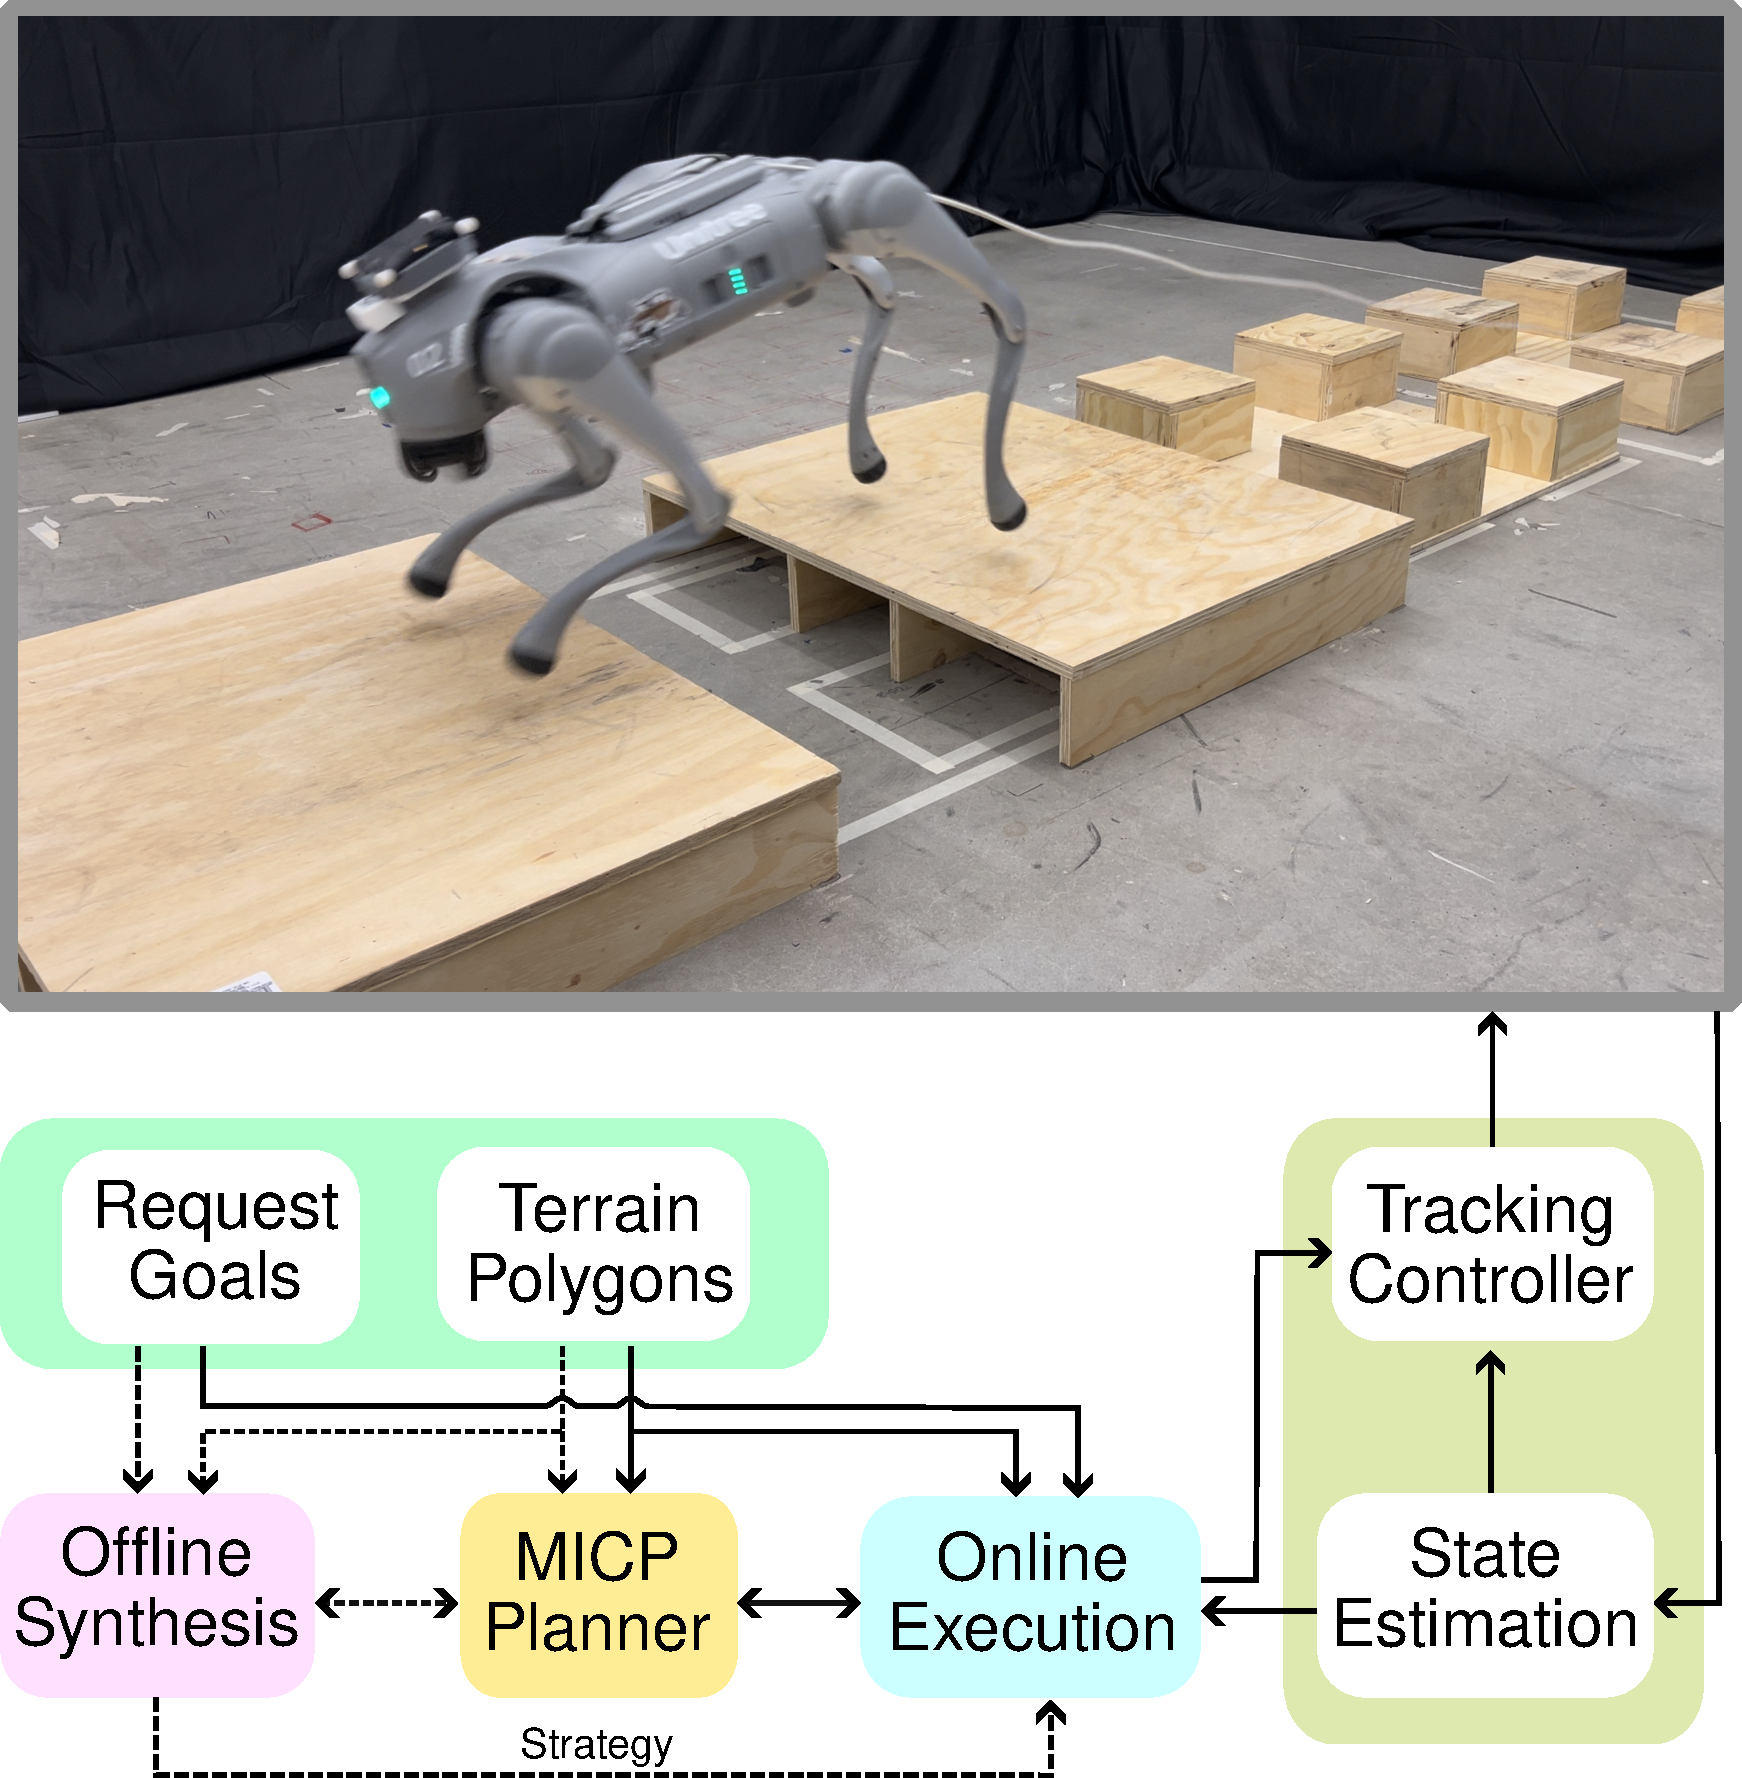
\includegraphics[width=1\linewidth]{system_diagram.pdf}
%     \caption{System architecture overview. The solid lines indicate online communication, while dashed lines represent offline processes.
%     }
%     \label{fig:system_diagram}
% \end{figure}
%%%%%%%%%%%%%%%%%%%%%%%%%%%%%%%%%%%

% \subsection{Reactive  Synthesis}
\subsection{Specifications}
% We use the Generalized Reactivity(1) (GR(1)) fragment of linear temporal logic (LTL)~\citep{bloem2012synthesis}
% to encode task specifications.
% LTL specifications $\spec$ 
% follow the grammar 
% $\spec \: := \var \:|\: \neg\: \spec \:|\: \spec \:\land\: \spec \:|\: \bigcirc\spec \:|\: \square \spec \:|\: \lozenge \spec$,
% where $\var \in \ap$ is an atomic proposition,
% $\neg$ ``not'' and $\land$ ``and'' are Boolean operators,
% and
% $\bigcirc$ ``next'',
% $\square$ ``always'',
% and $\lozenge$ ``eventually''
% are temporal operators.
% We refer the readers to~\citep{baier2008principles} for a detailed description of LTL.

% GR(1) specifications are expressed in the form of 
% $\spec = \envspec \to \sysspec$,
% where $\envspec = \envinit \land \envsafety \land \envlive$ 
% is the assumptions on the behaviors of the possibly adversarial environment,
% and $\sysspec = \sysinit \land \syssafety \land \syslive$
% represents the guarantee of the desired robot's behaviors.
% For $\alpha \in \{e, s\}$,
% $\alphainit, \alphasafety, \alphalive$
% characterize the 
% initial conditions,
% safety constraints,
% and liveness conditions,
% respectively.
% For symbolic repair (see Sec.~\ref{sec:manager_and_repair}),
% we divide safety constraints ($\envsafety, \syssafety$) into
% skill constraints ($\envsafetynothard, \syssafetynothard$)
% and hard constraints ($\envsafetyhard, \syssafetyhard$),
% i.e., for $\alpha \in \{e, s\}$,
% $\alphasafety = \alphasafetynothard \land \alphasafetyhard$.
% The skill constraints encode the pre and postcondition of skills 
% (see Sec.~\ref{sec:spec_gen})
% and can be modified by repair,
% while repair cannot modify the hard constraints.

We adopt the Generalized Reactivity (1) (GR(1)) fragment of linear temporal logic (LTL)~\citep{bloem2012synthesis} to encode task specifications.
An LTL formula $\spec$ follows the grammar
$\spec \: := \var \:|\: \neg\: \spec \:|\: \spec \:\land\: \spec \:|\: \bigcirc\spec \:|\: \square \spec \:|\: \lozenge \spec$,
where $\var \in \ap$ denotes an atomic proposition,
$\neg$ and $\land$ are Boolean operators,
and $\bigcirc$ (``next''), $\square$ (``always''), and $\lozenge$ (``eventually'') are temporal operators.
For a comprehensive introduction to LTL, we refer the reader to~\citep{baier2008principles}.

A GR(1) specification is written in the form $\spec = \envspec \to \sysspec$,
where $\envspec = \envinit \land \envsafety \land \envlive$ encodes the assumptions about the (possibly adversarial) environment,
and $\sysspec = \sysinit \land \syssafety \land \syslive$ represents the guarantees that define the system’s behavior.
For $\alpha \in \{e, s\}$, the components $\alphainit, \alphasafety, \alphalive$ describe the initial conditions, safety requirements, and liveness objectives, respectively.
\revised{We refer below and throughout the rest of this article to \emph{symbolic repair}, the process of augmenting the symbolic transition set with new, dynamically feasible skills whenever the current specification becomes unrealizable. The full procedure is formalized in Sec.~\ref{sec:manager_and_repair}; for the purpose of the upcoming definitions, it suffices to treat symbolic repair as a black box that proposes candidate symbolic transitions whose physical feasibility is then verified by MICP.}
In the context of symbolic repair (Sec.~\ref{sec:manager_and_repair}), we further partition the safety constraints ($\envsafety, \syssafety$) into two parts: skill-related constraints ($\envsafetynothard, \syssafetynothard$) and hard constraints ($\envsafetyhard, \syssafetyhard$).
The skill constraints encode the preconditions and postconditions of skills (see Sec.~\ref{sec:spec_gen}) and are subject to modification by the repair procedure, whereas the hard constraints remain immutable.

% We divide the environment safety assumptions $\envsafety$ into skill assumptions $\envsafetynothard$,
% which describe the postconditions of the skills (see Sec.~\ref{sec:spec_gen}),
% and hard assumptions $\envsafetyhard$ that cannot be modified
% ($\envsafety = \envsafetynothard \land \envsafetyhard$).
% Similarly, we split the safety guarantees $\syssafety$ into skill guarantees $\syssafetynothard$,
% which represent the preconditions of the skills,
% and hard guarantees $\syssafetyhard$ that cannot be modified
% ($\syssafety = \syssafetynothard \land \syssafetyhard$).


% \textbf{In practice, the size of the GR(1) specification $\spec$ for robotic applications is large.
% Since we may obtain more information at runtime,
% we can generate a partial evaluation, a shorter spec, at runtime.}

In practice, GR(1) specifications often become quite large because they must capture detailed information about both terrain and task constraints. At runtime, however, the exact terrain and request states are already available. This allows us to apply a technique known as partial evaluation originally defined in \citep{zhou2025physically}, where known Boolean propositions are directly substituted with their truth values. By doing so, we reduce the overall state space, leading to a smaller and more computationally efficient specification for synthesis.

\noindent\textbf{Definition~\deflabel{def:partial_eval}.}
Given an LTL formula $\spec$
and
two subsets $S^\true, S^\false \subseteq \ap$, $S^\true \cap S^\false = \emptyset$,
we define
the \textit{partial evaluation} of $\spec$ over $S^\true, S^\false$,
%denoted 
as $\spec[S^\true, S^\false]$, 
%to be
%$\spec[S^\true, S^\false] \coloneqq \spec [ \{\var \mapsto \true \mid \var \in S^\true\} \cup \{\var \mapsto \false \mid \var \in S^\false\} ]$.
%Intuitively, 
where we substitute 
propositions $\pi\in AP$ in $\spec$ with $\true$ if $\pi \in S^\true$ and with $\false$ if $\pi \in S^\false$.

%%%%%%%%% Problem statement and approach overview %%%%%%%%
\section{Problem Statement and Approach Overview}\label{sec:problem_statement}

\subsection{Problem Statement}
\textbf{Problem~\problemlabel{problem:1}}.
Given
\begin{enumerate*}[label=(\roman*),ref=\roman*]
    \item a global goal $g_{\textrm{global}}$,
    \item a set of possible local request goals $\mathcal{G}_{\textrm{local}}$
    \item a set of predefined terrain polygons $\mathcal{P}_{\text{pre}}$ from user's prior knowledge,
    and
    \item a set of online terrain polygons $\mathcal{P}_{\text{on}}$ perceived during execution that may differ from the predefined ones,
    \item a set of predefined locomotion gaits $\mathcal{L}$;
\end{enumerate*}
generate controls that enable the robot to navigate the environment and reach the goal.

\subsection{Approach Overview}\label{sec:approach_overview}
To address Problem~\ref{problem:1} efficiently, we manage complexity on both symbolic and physical levels. At the symbolic level, we employ reactive synthesis to break down the local navigation task into smaller subproblems, which can be reused across different scenarios. Each subproblem involves planning a short-horizon symbolic transition and is accompanied by solving a MICP to certify its physical feasibility.

As shown in Fig.~\ref{fig:system_diagram}, our overall framework is composed of three main modules: offline synthesis (Sec.~\ref{sec:reactive_gait_synthesis}), online execution (Sec.~\ref{sec:online_execution}), and low-level tracking control (Sec.~\ref{sec:tracking_control}). During offline synthesis, we generate a diverse set of locomotion skills and their associated gaits for various predefined terrain-task combinations. Symbolic repair is applied to discover additional necessary transitions that may not be captured initially.

At runtime, we invoke a symbolic repair mechanism to synthesize new transitions when the robot encounters unexpected terrain conditions or request goals not seen during offline planning. This allows the framework to remain flexible and adaptive to evolving environments. \revised{Additionally, the system re-targets the desired pose during each transition to reflect current terrain constraints, and coordinates the strategy automaton with the tracking controller to handle MICP solve-time variability without compromising execution continuity.}


%%%%%%%%% Offline synthesis %%%%%%%%
\section{Offline Synthesis}\label{sec:reactive_gait_synthesis}
% The offline synthesis module 
% generates a strategy 
% that enables the robot
% to reach desired goal waypoints over all predefined terrain states.
% As shown in Fig.~\ref{fig:combined_offline_online}(a),
% this module takes in
% a set of request goals and
% a set of possible terrain states from prior knowledge of the workspace. In addition, a set of locomotion gaits is also provided by the user. After discretizing the local environment and characterizing the terrains in Sec.~\ref{sec:preliminaries_abstraction}, we first solve a gait-fixed MICP problem to determine the feasibility of each potential skill given the locomotion gaits
% (Sec.~\ref{sec:motion_primitive}), and then encode all feasible transitions as skills in a specification
% (Sec.~\ref{sec:spec_gen}).
% If the specification is realizable, we generate a strategy for online execution.
% Otherwise, we leverage a repair process to suggest new robot skills, utilize the gait-free MICP planner to check the feasibility of the suggested skills, and eventually make the specification realizable
% (Sec.~\ref{sec:symbolic_repair}).
%%%% Fig4. System overview %%%%
\begin{figure*}[ht]
    \centering
    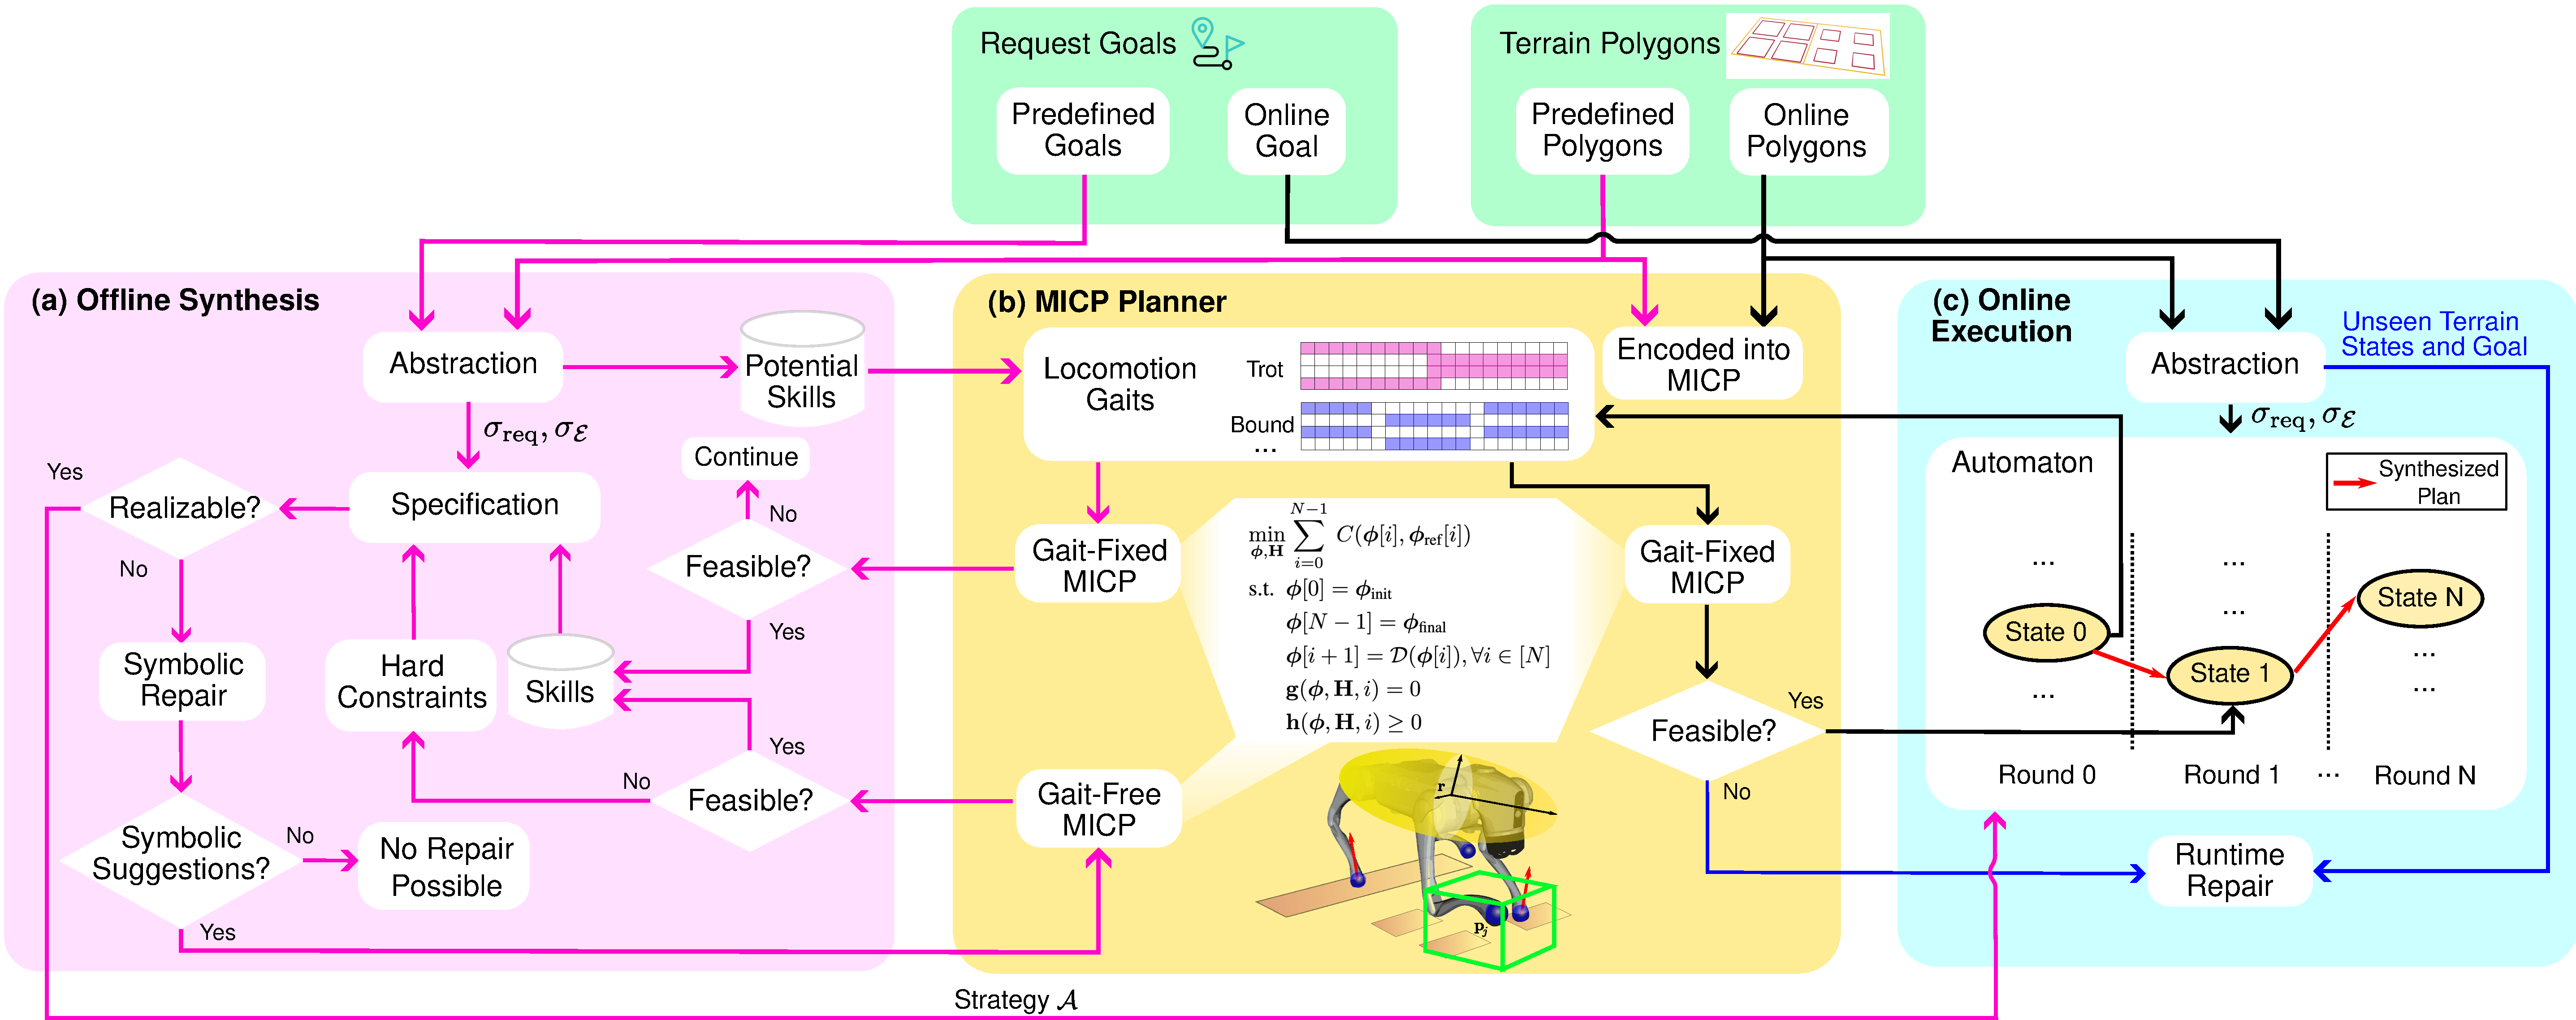
\includegraphics[width=\linewidth]{combined_offline_online_v2.pdf}
    \caption{System overview.  
    % for offline synthesis and online execution. 
    During offline synthesis (pink arrows), an initial set of locomotion gaits is provided, and symbolic skills are iteratively generated by solving the MICP. When the task specifications are unrealizable, a symbolic repair is triggered to seek missing skills.
    During the online execution (black arrows), MICP is solved again taking online terrain segments and the symbolic state only advances when a solution is found.
    % During online execution (black arrows), the MICP is solved again using incoming terrain segments, and the symbolic state is advanced only once a valid solution is obtained. 
    A runtime repair (blue arrows) is initiated if a solving failure occurs, 
    or an unseen terrain or request goal is encountered.
    }
    \label{fig:combined_offline_online}
    \vspace{-0.1in}
\end{figure*}
%%%%%%%%%%%%%%%%%%%%%%%%%%%%%%%%%%%

The offline synthesis module builds a strategy that allows the robot to reach local request goals under predefined terrain conditions. As shown in Fig.~\ref{fig:combined_offline_online}(a), the module takes in local request goals $\mathcal{G}_{\textrm{local}}$, terrain polygons $\mathcal{P}_{\text{pre}}$ from prior maps, and a set of locomotion gaits $\mathcal{L}$ specified by the user.
We first apply the inverse grounding function $\inversegrounding$ to discretize the local environment, deriving a set of candidate request states $\inpstatesrequestposs \subseteq \inpstatesrequest$ from the local request goals and mapping the predefined terrain polygons into possible terrain states $\inpstatesterrainexprposs \subseteq \inpstatesterrain$.
Afterward, we evaluate the feasibility of each candidate skill using a gait-fixed MICP formulated with the provided locomotion gaits (Sec.~\ref{sec:motion_primitive}), and record all feasible transitions as symbolic skills in the specification (Sec.~\ref{sec:spec_gen}).
To improve efficiency, a high-level manager then generates partial evaluations of the encoded specifications. Whenever one of these partial evaluations is deemed unrealizable, a repair mechanism is invoked: it proposes additional symbolic skills, whose feasibility is validated through gait-free MICP. This process ensures that the specification ultimately becomes realizable (Sec.~\ref{sec:manager_and_repair}).
% We first 
% use the inverse grounding function $\inversegrounding$ to 
% discretize the local environment,
% obtain
% a set of possible
% request states $\inpstatesrequestposs \subseteq \inpstatesrequest$
% from the local request goals,
% and characterize the predefined set of terrain polygons into a set of possible terrain states $\inpstatesterrainexprposs \subseteq \inpstatesterrain$.
% Next, 
% we solve a gait-fixed MICP problem to determine the feasibility of each potential skill given the locomotion gaits
% (Sec.~\ref{sec:motion_primitive}), and then encode all feasible transitions as skills in a specification
% (Sec.~\ref{sec:spec_gen}).
% Next,
% we use a high-level manager to 
% generate partial evaluations of the encoded specifications
% for efficient synthesis.
% If any partial evaluation is unrealizable, 
% we leverage a repair process to suggest new symbolic-level robot skills 
% and a gait-free MICP to verify the feasibility of the suggested skills, 
% eventually making the specification realizable
% (Sec.~\ref{sec:manager_and_repair}).


% The reactive synthesis process has two phases: offline synthesis and online execution. 
% We begin by introducing the essential specifications that define our terrain-adaptive locomotion problem. The objective is to construct a high-level robot gait and keyframe transition strategy by solving a two-player game between the gait planner and its possibly adversarial environment. The Linear Temporal Logic (LTL) specifications are designed by human experts, who provide logical rules that guide the planning process. It is nothworthy that the specification design is not unique and may vary according to expert input.

% Add a mapping function from the discrete state to the continuous state?

% \subsection{Motion Primitives to Robot Skills}\label{sec:motion_primitive}
\subsection{Locomotion Gait and Feasibility Checking via MICP}\label{sec:motion_primitive} 
We assume each locomotion gait $L$ is characterized by a contact sequence $\mathcal{G}$ and its associated time durations $T$, formally written as $L = \mathcal{M}(\mathcal{G}, T)$. Each skill is tied to a distinct locomotion gait, which dictates how the robot executes motion at the continuous level.
As illustrated in Fig.~\ref{fig:combined_offline_online}(a), since the offline phase has access to the complete set of request states $\inpstatesrequestposs$ and terrain states $\inpstatesterrainexprposs$, we can systematically enumerate all possible symbolic skills that enable navigation across the different local environments. The feasibility of each skill is then evaluated through gait-fixed MICP using the given locomotion gaits.
% We assume each locomotion gait comes with a contact sequence $\mathcal{G}$ and corresponding time durations $T$. Therefore, we define the locomotion gait as $L = \mathcal{M}(\mathcal{G}, T)$. Each skill is assumed to have a unique locomotion gait to determine how the robot moves at the continuous level. 
% As shown in Fig.~\ref{fig:combined_offline_online}(a), since all the possible request goals $\inprequest$ and terrain states $\inpterrain$ are predefined during the offline phase, it is straightforward to first identify all the potential skills at the symbolic level that allow the robots to move freely in all possible local environments. 
In most examples shown in this paper, we assume the robot is only allowed to move horizontally and vertically by one cell and we show diagonal movements and heading angle change in Sec.~\ref{sec:extension}.
% Then, 
% we formulate a MICP problem that
% each MICP solve can 
% takes in 

Then the next critical step is to find whether there exists a locomotion gait for each skill to be physically feasible.
We leverage mixed-integer convex programming (MICP) to check the physical feasibility given a set of predefined locomotion gaits, and only use the feasible one as robot skills to synthesize robot strategies. The MICP problem takes in
the centroidal states $\inpcen$ from the precondition and postcondition of the skill as its initial and final conditions, which are located at the center of each abstracted cell. A set of homogeneous, predefined terrain polygons are considered in the MICP as steppable regions corresponding to the terrain states $\inpterrain$ involved in the precondition. Lastly, the contact information $\mathcal{G}$ and $T$ is provided by the selected locomotion gait $L$. Fig.~\ref{fig:mip_go2} shows the maneuver of the quadruped robot Go2 after solving the MICP problem corresponding to skill $a_0$ in Example~\ref{example:1} with a one-second trotting locomotion gait. The generic MICP problem considered in this work can formulated as:
    \begin{subequations}\label{ocp:mip_general}
    \begin{alignat}{2}
        \nonumber &\underset{\vg \phi, \v H}{\min} && \sum_{i = 0}^{N-1} \hspace{2pt} C(\vg \phi[i], \vg \phi_{\text{ref}}[i])\\
        & \text{s.t. } && \vg \phi[0] = \vg \phi_{\text{init}} \\& && \vg \phi[N-1] = \vg \phi_{\text{final}} \\
     & &&  \vg \phi[i+1] = \mathcal{D}(\vg \phi[i]), \forall i \in \range{N} \\
        & && \v g(\vg \phi, \v H, i) = 0 \\
        & && \v h(\vg \phi, \v H, i) \geq 0
    \end{alignat}
\end{subequations}
where the decision variables $\vg \phi$ denote the continuous variables and $\v H$ indicate the binary variables across the entire $N$ timesteps. For any natural number $n \in \naturals$, we denote the set $\{0, \dots, n-1\}$ as $\range{n}$. \revised{The function $\mathcal{D}(\cdot)$ encodes the discrete-time system dynamics that propagate the continuous state $\vg \phi[i]$ to $\vg \phi[i+1]$; the specific dynamics used in this work are detailed in Eq.~(\ref{eq:dynamics}).} The general equality constraints $\v g(\cdot)$ and inequality constraints $\v h(\cdot)$ are incorporated and activated at certain time stamp $i$. The cost function depends on both the continuous variables $\vg \phi$ and a reference trajectory $\vg \phi_{\text{ref}}$.

\begin{figure}
    \centering
    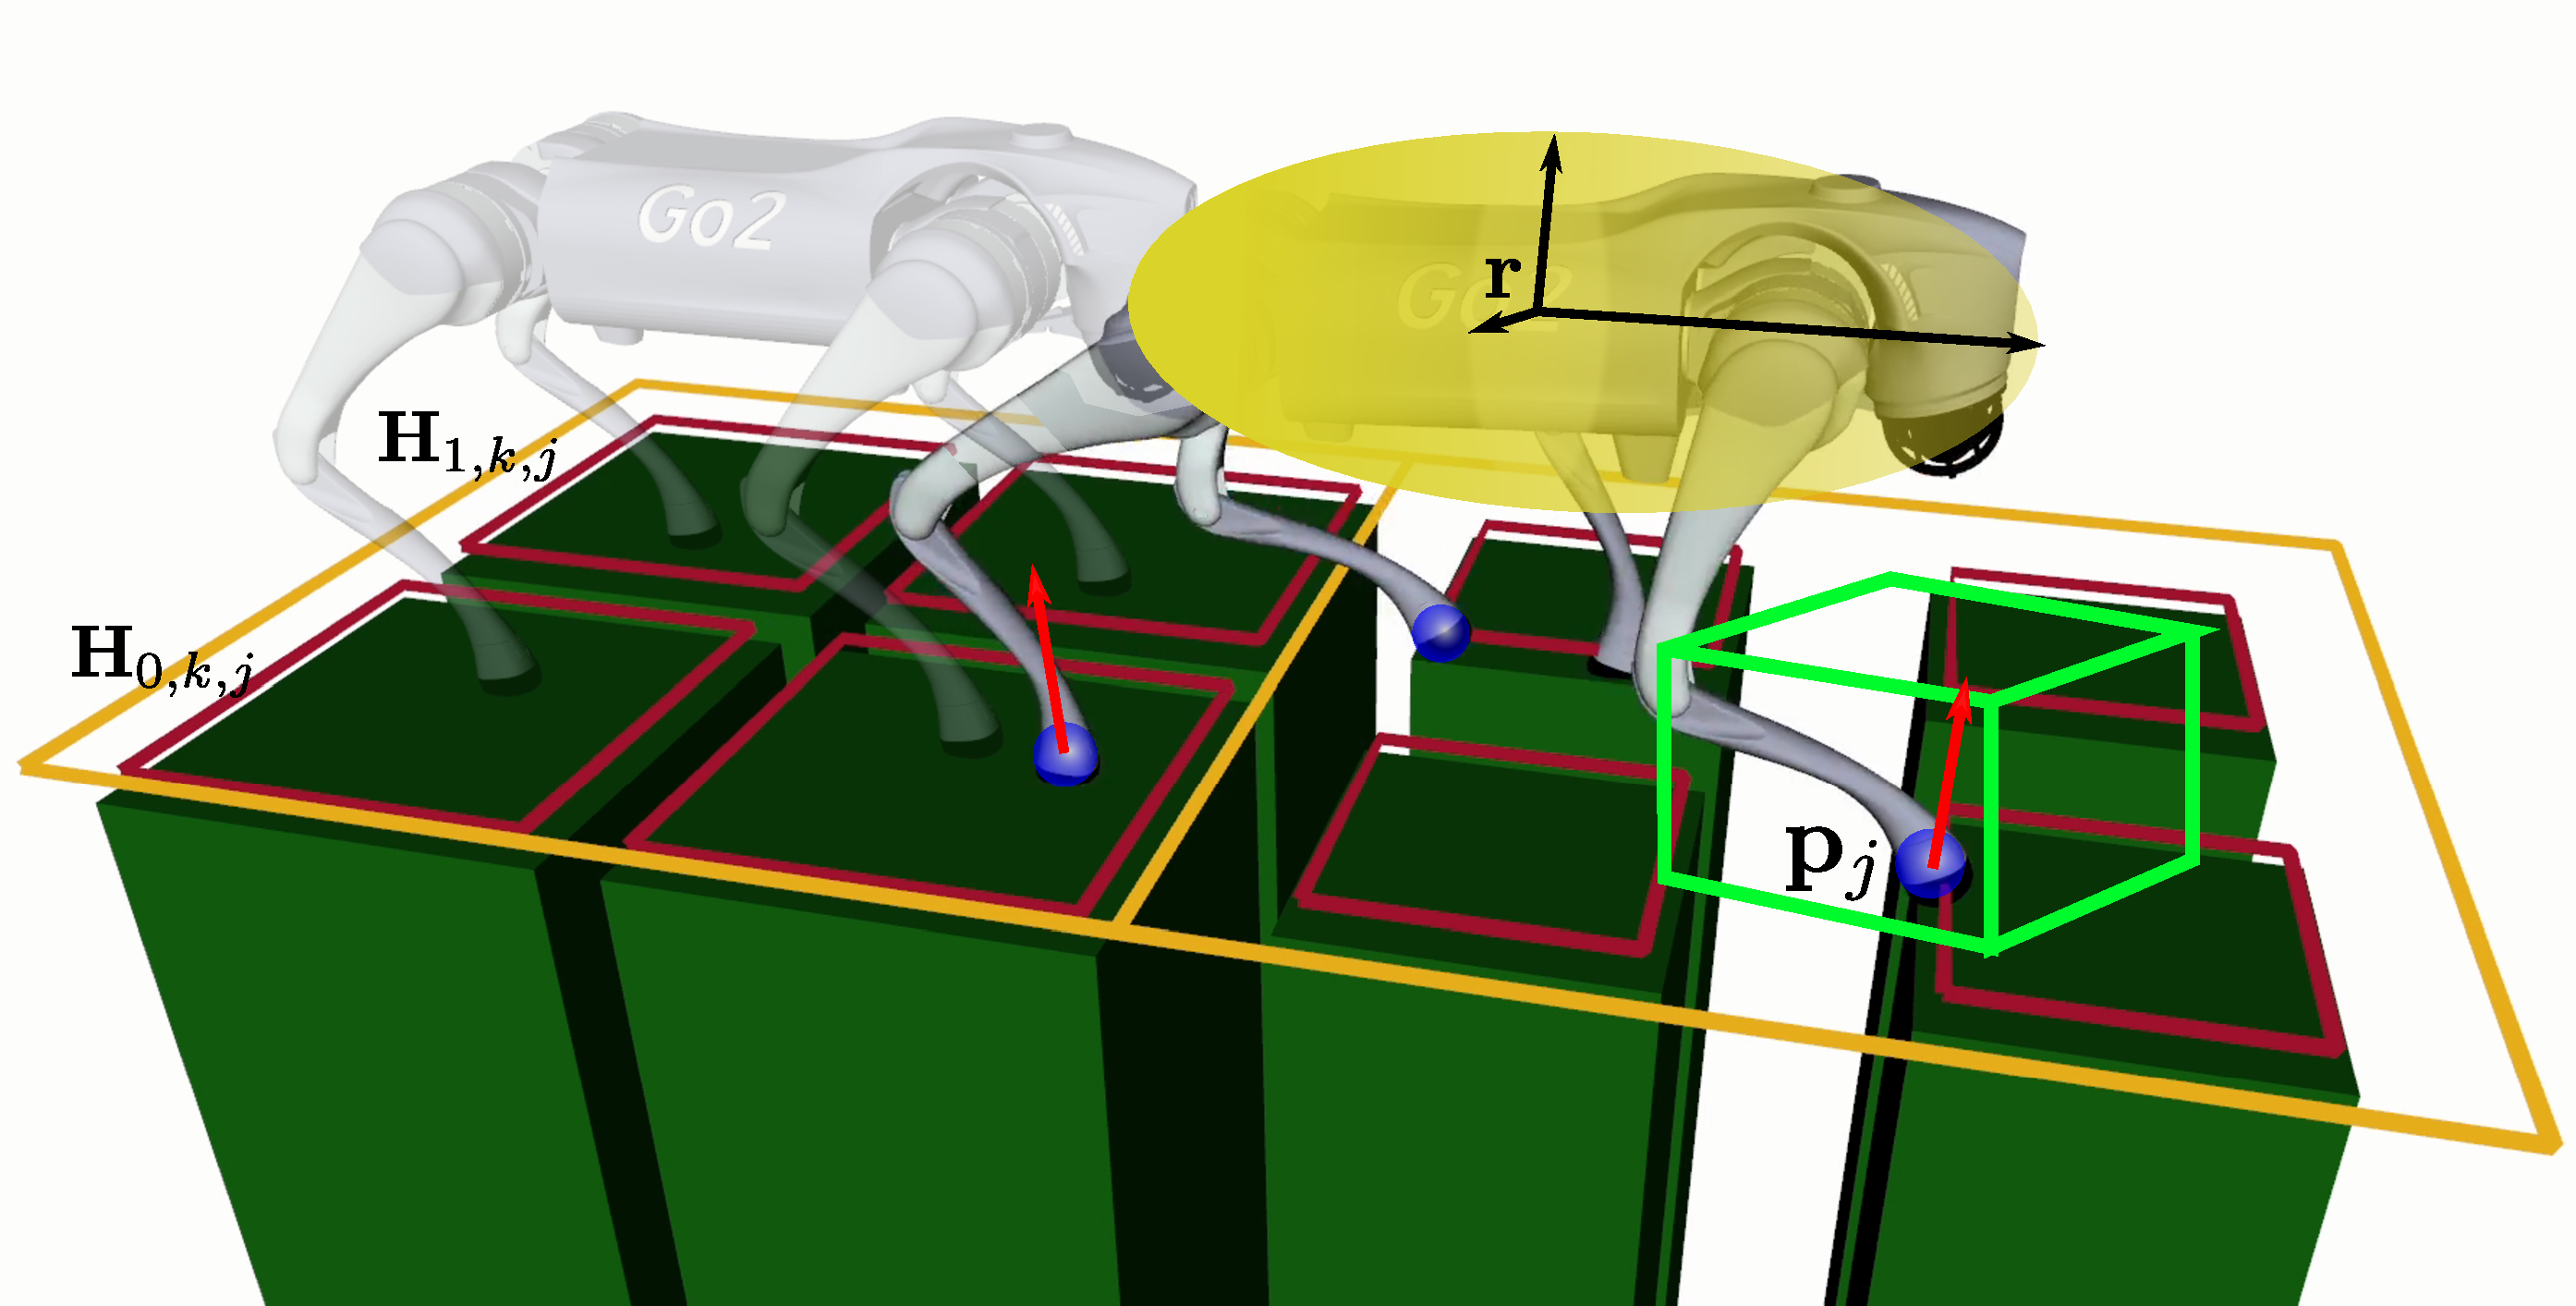
\includegraphics[width=0.9\linewidth]{mip_go2.pdf}
    \caption{Demonstration of decision variables and polygons when solving MICP for skill $a_0$ in Example~\ref{example:1} using a trotting locomotion gait.}
    \label{fig:mip_go2}
\end{figure}

The reference base position and angular trajectories are generated by linearly interpolating between the initial and final conditions. For scenarios with significant elevation changes, such as jumping onto higher terrain, an additional middle keyframe is introduced for the pitch angle to calculate the slope angle between the initial and final poses. The final reference pitch trajectory is then created by evenly interpolating between the initial, middle, and final poses. The reference EE trajectory relative to the base frame $^\mathcal{B} \v p_j^{\text{ref}}$ remains constant and moves in sync with the reference base trajectory. Given a specific locomotion gait, we first introduce the gait-fixed MICP formulation:

\subsubsection{Continuous Decision Variables}
The continuous decision variables $\vg \phi$ include base position $\v r$, velocity $\dot{\v r}$, acceleration $\ddot{\v r}$, orientation $\vg \theta$ parameterized by Euler angle and its first and second-order derivatives $\dot{\vg \theta},\ddot{\vg \theta}$, individual end-effector (EE) position $\v p_j$, velocity $\dot{\v p}_j$, and acceleration $\ddot{\v p}_j$, and individual contact force $\v f_j$ for the foot $j$ with $j\in\range{n_f}$, where $n_f=4$ denotes the index of feet. The compact form can be expressed as:
\begin{equation}
    \vg \phi = [\v r^\top, \dot{\v r}^\top, \ddot{\v r}^\top, \vg \theta^\top, \dot{\vg \theta}^\top, \ddot{\vg \theta}^\top, \v p_j^\top, \dot{\v p}_j^\top, \ddot{\v p}_j^\top, \v f_j^\top]^\top
\end{equation}

\subsubsection{System Dynamics}
We encode the system dynamics as a simplified single rigid body in Eq.~(\ref{eq:dynamics}),
using a double integrator to replace the original Euler equation to keep the dynamics constraint convex. The whole system is discretized through Backward Euler integration with $\Delta t$ between each time step.
\begin{equation}
        \label{eq:dynamics}
        \begin{bmatrix} \v r[i+1]\\\
        \dot{\v r}[i+1]\\\
        m \ddot{\v r}[i]\\\
        \vg \theta[i+1]\\
        \dot{\vg \theta}[i+1]
        \end{bmatrix}= \begin{bmatrix}
        \v r[i] + \Delta t \cdot \dot{\v r}[i+1]\\
        \dot {\v r}[i] + \Delta t \cdot \ddot{\v r}[i+1]\\
        \sum\nolimits_{j} \v f_j[i] + m \v g \\
	    % \sum\nolimits_j (\v{p}_j[i] - \v r[i]) \times \v f_j[i] \\
            \vg \theta[i] + \Delta t \cdot \dot{\vg \theta}[i+1]\\
            \dot{\vg \theta}[i] + \Delta t \cdot \ddot{\vg \theta}[i+1]
	    \end{bmatrix}
\end{equation}
where $m$ is the robot mass and $g$ is the gravity term.

\revised{We note that the rotational dynamics adopted in Eq.~(\ref{eq:dynamics}) are intentionally simplified: the rotational equation of motion is replaced by a double integrator on the Euler angles, which keeps the constraint convex but \textit{neglects the true angular-momentum dynamics.} This makes the formulation tractable for online deployment, but it limits applicability to highly dynamic motions such as flips or aggressive yaw maneuvers at high speeds.
%, or platforms where angular-momentum management is critical (e.g., humanoids).
Future work will explore convex relaxations of the full angular-momentum dynamics to expand the range of feasible motions while maintaining online tractability.}

\subsubsection{Cost Function}
The cost function consists of tracking costs and regularization terms governed by diagonal matrices $\v Q$ and $\v R$. 
\begin{equation}
    \v C = \delta \vg \phi_Q[i]^T\mathbf{Q}\hspace{2pt}\delta \vg \phi_Q[i] + \vg \phi_R[i]^{T}\mathbf{R}\vg \phi_R[i]
\end{equation}
where $\delta \vg \phi_Q$ and $\vg \phi_R$ are defined as:
\begin{equation}
    \delta \vg \phi_Q = \begin{bmatrix}
        \v r - \v r_{\text{ref}}\\
        \vg \theta - \vg \theta_{\text{ref}}\\
        \v p_j - \v p_{j}^{\text{ref}}
    \end{bmatrix}, \vg \phi_R = \begin{bmatrix}
        \ddot{\v r}\\
        \ddot{\vg \theta}\\
        \ddot{\v p}_j\\
        \v f_j
    \end{bmatrix}
\end{equation}

Tracking costs include deviation from the desired base and foot EE trajectories. The regularization term includes minimizing the base acceleration, Euler angle acceleration, EE acceleration, and contact forces to encourage motion smoothness. The weights for the tracking terms are defined in Table~\ref{tab:cost_weights}.

% \qm{plz also explain $N, n_f, n_s,$ and $R$}

% \subsubsection{Collision Avoidance}

\subsubsection{Safe Region Constraint}
To incorporate safe region constraints for selecting proper footholds, we introduce binary variables $\v H_{r,k,j}$, with $r$, $k$, and $j$ expressing the $r^{\rm th}$ convex region, $k^{\rm th}$ footstep, and $j^{\rm th}$ foot and $r\in\range{R}, k\in\range{n_s}$. One footstep is defined as a full swing phase for a foot. We use $n_s$ and $R$ to represent the number of footsteps specified by the gait configuration and the number of convex terrain polygons to be considered. For example,  Fig.~\ref{fig:mip_go2} shows a case with eight polygons.
Eqs.~(\ref{eq:safe_region}) - (\ref{eq:safe_region_eq}) restrict
the robot's EE to stay within one of the convex polygons when the corresponding binary variable $\v H_{r,k,j}$ is True. 
Each polygon is parameterized by an inequality constraint ($\v A_r$ and $\v b_r$) that defines multiple half-spaces, along with an equality constraint ($\v A_{\text{eq},r}$ and $\v b_{\text{eq},r}$) that ensures the foothold position lies on a 3D plane.
We use $\mathcal{C}_{k,j}$ to denote the set of time steps indicating stance after the $k^{\rm th}$ footstep for the $j^{\rm th}$ foot and the safe region constraint only applies to the first stance time step represented as $\mathcal{C}_{k,j}[0]$. Note that, during the offline phase, the terrain polygons are homogeneous and predefined.
\begin{align}
\nonumber
&\forall r \in [R], k \in [n_s], j \in [n_f]\\
    \label{eq:safe_region} &\v H_{r,k,j} \Rightarrow \v A_r \v p_j[i] \leq \v b_r, \forall i \in \mathcal{C}_{k,j}[0]
        \\\label{eq:safe_region_eq} & \hspace{1.5cm} \v A_{\text{eq},r} \v p_j[i] = \v b_{\text{eq},r}, \forall i \in \mathcal{C}_{k,j}[0]
        \\\label{eq:sum_contact_binary} &\sum_{r=0}^{R-1}\v H_{r,k,j} = 1
        \\&\v H_{r,k,j} \in \{0, 1\}
\end{align}

\subsubsection{Frictional and Contact Constraints}
Frictional constraints are defined in Eqs.~(\ref{eq:force_non_zero}) - (\ref{eq:force_friction_cone}), with $\v n_r$ and $\mathcal{F}_r$ as the normal vector and friction cone of the $r^{\rm th}$ convex region corresponding to the x and y dimensions of the EE position $\v p^{xy}_j$. Contact constraints in Eqs.~(\ref{eq:ee_velocity_zero}) - (\ref{eq:force_zero}) forces the EE velocity to be zero during stance phase and the contact force to be zero during the non-contact phase. $\mathcal{C}_{j}$ represents the set of all time steps indicating stance for the $j^{\rm th}$ foot.
\begin{align}
    \nonumber &\forall r \in [R], k \in [n_s], j \in [n_f]\\\label{eq:force_non_zero}
    &\v H_{r,k,j} \ \  \Rightarrow \ \ \v f_j[i] \cdot \v n_r(\v p_j^{xy}[i]) \ge 0, \ \forall i \in \mathcal{C}_{k,j}\\
    \label{eq:force_friction_cone}
        & \hspace{1.95cm} \v f_j[i] \in \mathcal{F}_r(\mu, \v n_r, \v p_j^{xy}[i]), \ \forall i \in \mathcal{C}_{k,j}
         \\\label{eq:ee_velocity_zero}
            &\dot{\v p}_j[i]=0, \ \forall i \in \mathcal{C}_j
        \\\label{eq:force_zero}
         &\v f_j[i] = 0, \ \forall i \notin \mathcal{C}_j
\end{align}
%
where $\mu$ denotes the friction coefficient.

\subsubsection{Actuation Constraint}
Since the joint angles are omitted in the single rigid body model, we use a fixed Jacobian $\v J_j(\v q_j^{\text{ref}})$ at a nominal joint pose $\v q_j^{\text{ref}}$ for each leg to approximately consider the torque limit constraint in Eq.~(\ref{eq:max_torque}). In addition, since the translational and angular motions are decoupled, another actuation constraint on the angular acceleration is also added in Eq.~(\ref{eq:max_acc}).
\begin{align}
\nonumber & \forall i \in [N], j \in [n_f] \\
    \label{eq:max_torque}
& \v J_j(\v q_j^{\text{ref}})^{\top} \v f_j[i] \leq \vg \tau_{\rm max}\\\label{eq:max_acc}
& \v I \ddot{\vg \theta}[i] \leq \vg \tau_{\rm max}^{\prime}
\end{align}
where $\vg \tau_{\rm max}$ is the joint torque limit, $\vg \tau_{\rm max}^{\prime}$ is the torque limit applied on the base, and $\v I$ is the moment of inertia for the approximated single rigid body.

\subsubsection{Kinematics Constraint}
Lastly, the kinematics constraint in Eq.~(\ref{eq:rom}) strictly limits the possible EE movements to assure safety.
% Fig.~\ref{fig:mip_a1} shows the essential decision variables optimized in \ref{ocp:mip_general}. 
Due to the convex nature of this MICP, we can determine the feasibility of a possible symbolic transition by checking if the optimal solution exists.
\begin{equation}
    \label{eq:rom}
    \v p_j[i] \in \mathcal{R}_j(^\mathcal{B} \v p_j^{\text{ref}}, \v r[i],\vg \theta_{\text{ref}}, \v p_j^{\text{max}}), \forall i \in [N], j \in [n_f]
\end{equation}
where $\mathcal{R}_j$ is defined as a 3D box constraint around a nominal foot EE position based on the base position and orientation, and constrained by a maximum deviation $\v p_j^{\text{max}}$. Note that the reference orientation $\vg \theta_{\text{ref}}$ is used to avoid nonlinear constraint keep the problem convex.

% \subsection{GR(1) Specifications given Robot Skills}\label{sec:spec_gen}
% \subsection{Task Specification Encoding}\label{sec:spec_gen}

% After acquiring a set of feasible robot skills, 
% we encode the skills into the specification $\spec$ 
% as part of the environment safety assumptions $\envsafety$ 
% and system safety guarantees $\syssafety$.
% %
% % We divide the safety assumptions $\envsafety$ into mutable assumptions $\envsafetynothard$,
% % which describe the postconditions of the skills,
% % and hard assumptions $\envsafetyhard$ that cannot be modified, 
% % i.e.
% % $\envsafety = \envsafetynothard \land \envsafetyhard$.
% % Similarly, we divide the safety guarantees $\syssafety$ into mutable guarantees $\syssafetynothard$,
% % which represent the preconditions of the skills,
% % and hard guarantees $\syssafetyhard$ that cannot be modified
% % ($\syssafety = \syssafetynothard \land \syssafetyhard$).
% %
% % To translate from states to formulas, 
% We define a function $\formplain$ that takes as input
% two subsets $\statevar, \statevar' \subseteq \ap$,
% where $\statevar \subseteq \statevar'$,
% and generates a Boolean formula
% $\form{\statevar'}{\statevar} \coloneqq \bigwedge_{\var\in\statevar}\var \land \bigwedge_{\var \in \statevar'\setminus\statevar} \neg\var$.
% For any subset $\statevar \subseteq \ap$,
% we use $\bigcirc\statevar$ to denote the set $\{\bigcirc \pi \mid \pi \in \statevar\}$.

% % We encode the postconditions of the skills into the environment safety assumptions $\envsafety$ of the specification $\spec$.



% % each skill $\texttt{skill} \in \mathcal{A}$ comes with a precondition $\sum_{\texttt{skill}}^{\rm{pre}} \in 2^{\mathcal{I}_G}$ and a postcondition $\sum_{\texttt{skill}}^{\rm{post}} \in 2^{\mathcal{I}_G}$ similar to \citep{pacheck2022physically}. In Fig.~\ref{fig:preliminary_nine_squares}(b) and (c), it shows a skill $\texttt{skill0}$ with precondition $\sum_{\texttt{skill0}}^{\rm{pre}} = \{(x=1,y=2,\rm cT = \rm Flat, \rm rT = \rm High)\}$ and postcondition $\sum_{\texttt{skill0}}^{\rm{post}} = \{(x=2,y=2)\}$. The skills are encoded in the GR(1) formula as part of $\phi^\textrm{t}_\textrm{e}$ and $\phi^\textrm{t}_\textrm{s}$, 
% % which can be further divided into $\phi^{\textrm{t}}_{\textrm{e}} = \phi^{\textrm{t, mutable}}_{\textrm{e}} \wedge \phi^{\textrm{t, hard}}_{\textrm{e}}$ and $\phi^{\textrm{t}}_{\textrm{s}} = \phi^{\textrm{t, mutable}}_{\textrm{s}} \wedge \phi^{\textrm{t, hard}}_{\textrm{s}}$. $\phi^{\textrm{t, mutable}}_{\textrm{e}}$ and $\phi^{\textrm{t, mutable}}_{\textrm{s}}$ capture the postconditions and preconditions that the repair process might modify, respectively. $\phi^{\textrm{t, hard}}_{\textrm{e}}$ and $\phi^{\textrm{t, hard}}_{\textrm{s}}$ encode the hard constraints specified by the user remain unchanged and always hold.   

% % \subsubsection{Postconditions}
% The skill assumptions $\envsafetynothard$ encode the postconditions of the skills. 
% % As shown in Eq.~\ref{eq:env_trans}, 
% The assumptions ensure that after the skill execution, 
% at least one postcondition of the skill must hold:
% % s in the next timestep:

% \begin{equation}\label{eq:env_trans}
% \begin{aligned}
%     \envsafetynothard \coloneqq \bigwedge_{\skill \in \mathcal{O}} \big( \skill 
%     % \land 
%     % \form{\inpcen\cup\inpterrain}{\skillpre} \\ 
%     \to
%     \bigvee_{\statevar\in\skillpost} \form{\bigcirc\inpcen}{\bigcirc\statevar} \big)
%     % \bigvee_{\sigma_\textrm{pre} \in \sum_{\texttt{skill}}^\textrm{pre}} \varphi_{\sigma_{\textrm{pre}}}) \rightarrow \\
%     % &\bigcirc \bigvee_{\sigma_\textrm{post} \in \sum_{\texttt{skill}}^\textrm{post}} \varphi_{\sigma_\textrm{post}}\bigg)
% \end{aligned}
% \end{equation}
% %
% In Example~\ref{fig:preliminary_nine_squares},
% % $\skillprecustom{\skillcustom{0}}$,
% the postcondition of skill $\skillcustom{0}$
% is defined as:
% % encoded asin Eq.~\ref{eq:skill_0_post}:
% % Therefore, as an example, the postcondition specification for $\texttt{skill0}$ is defined as:
% \begin{equation}\label{eq:skill_0_post}
% \begin{aligned}
%      \square (\skillcustom{0} 
%      % \land x_1 \land y_1 \land \tvar{x_1}{y_0} \land \tvar{x_1}{y_1} \land \tvar{x_1}{y_2}
%      % \land \bigwedge_{\var\in\inpcen\cup\inpterrain\setminus\skillprecustom{\skillcustom{0}}} \neg \var \\
%     \to &\bigcirc x_0 \land \bigcirc y_1 \land \neg \dots)
%     % &\neg \bigcirc x_1 \land 
%     % \neg \bigcirc x_2 \land 
%     % \neg \bigcirc y_0 \land 
%     % \neg \bigcirc y_2 \big)
%      % \bigwedge_{\var\in\inpcen\setminus\skillpostcustom{\skillcustom{0}}} \neg \bigcirc \var \big)
%      % x=1 \wedge y=2 \wedge \rm cT = \rm Flat \wedge \rm rT = \rm High \big) \rightarrow \\
%      % &\bigcirc \big(x=2 \wedge y=2 \big) \big)
% \end{aligned}
% \end{equation}
% where we omit the centroidal inputs that are False.

% % \subsubsection{Preconditions}
% The skill guarantees $\syssafetynothard$ encode the preconditions of the skills.
% The guarantees impose restrictions on when a skill can be executed.
% % As shown in Eq.~\ref{eq:sys_trans},
% The guarantees only allow the robot to execute a skill 
% if one of the skill's preconditions holds:
% % The preconditions encode constraints in $\varphi_{\textrm s}^{\textrm{t}, \textrm{mutable}}$. It restricts the conditions that a specific skill can be chosen. Therefore, it allows the overall system to choose a skill only when a precondition is satisfied, but does not require the system to do so. 

% \begin{equation}\label{eq:sys_trans}
% \begin{aligned}
%     \syssafetynothard \coloneqq 
%     \bigwedge_{\skill \in \mathcal{O}} \bigg(
%     \neg \big(
%     \bigvee_{\statevar\in\skillprecustom{\skill}}
%     \form{\bigcirc\inpcen\cup\bigcirc\inpterrain}{\bigcirc\statevar}
%     \big)
%     % \\
%     % \form{\bigcirc(\inpcen\cup\inpterrain)}{\bigcirc\skillprecustom{\skill}}\\
%     \to \neg \bigcirc \skill
%     \bigg)
%     % \\
%     % \varphi_{\textrm s}^{\textrm{t}, \textrm{mutable}} = \bigwedge_{\pi_{\texttt{skill}} \in \mathcal{O}} \bigg( & \neg (\bigcirc \bigvee_{\sigma_\textrm{pre} \in \sum_{\texttt{skill}}^\textrm{pre}} \varphi_{\sigma_{\textrm{pre}}}) \rightarrow 
%     % &\neg \bigcirc \pi_{\texttt{skill}}\bigg)
% \end{aligned}
% \end{equation}
% %
% In Example~\ref{example:1}, the precondition of skill $\skillcustom{0}$ is defined as:
% \begin{equation}
% \begin{aligned}
%      \square \big( \neg 
%      (
%      \bigcirc x_1 \land 
%      \bigcirc y_1 \land 
%      \bigcirc \tvar{x_1}{y_0} \land 
%      \bigcirc \tvar{x_1}{y_1} \land 
%      \bigcirc \tvar{x_1}{y_2}\land \\
%      \neg \dots)
%      % \neg \bigcirc x_0 \land
%      % \neg \bigcirc x_2 \land
%      % \neg \bigcirc y_0 \land
%      % \neg \bigcirc y_2 \land \\
%      % \bigwedge_{i\in\{0,2\}, j\in\{0,1,2\}}
%      % \neg \bigcirc \tvar{x_i}{y_j}\big)
%      % \bigwedge_{\var\in\inpcen\cup\inpterrain\setminus\skillprecustom{\skillcustom{0}}} \neg \bigcirc \var
%      % \big)
%      % \\
%      \to \neg \bigcirc \skillcustom{0} \big)
%      % \\
%      % (\bigcirc (x=1 \wedge y=2 \wedge \rm cT = \rm Flat \wedge \rm rT = \rm High)) \rightarrow \\
%      % \neg \bigcirc \pi_\texttt{skill0}\big)
% \end{aligned}
% \end{equation}
% where we omit the centroidal and terrain inputs that are False.
% % include the keyframe transition action $\mathcal{K}$ and gait primitives $\mathcal{G}$. We further divide $\mathcal{G}$ into $\mathcal{G} = \{\rm{gaitType}, \rm{gaitSpeed}\}$. We incorporate extra input propositions $\mathcal{E}$ to represent the terrain information, which shows up in the preconditions as well.
% % \subsubsection{Hard Constraints}\label{sec:hard_constraints}

% The hard constraints ($\envsafetyhard$, $\syssafetyhard$) are constraints that a repair cannot modify 
% (see Sec.~\ref{sec:symbolic_repair}).
% To strictly guarantee $\syssafetyhard$,
% we only allow the robot to execute one skill at a time:
%     $\square\big(\neg (\bigcirc\skill \land \bigcirc\skill')\big)$, for any two different skills $\skill, \skill' \in \out$. Given that, 
%     %such that $\skill \neq \skill'$.
% we encode the following hard assumptions $\envsafetyhard$:
% % as hard constraints in $\envsafetyhard$ and $\syssafetyhard$:
% % The hard assumptions $\envsafetyhard$ states that
% \begin{enumerate}[label=\arabic*),ref=\arabic*]
%     \item The uncontrollable terrain and request inputs 
%     % $\inpterrain \cup \inprequest$
%     % which include the terrain and request inputs ($\inpuser = \inpterrain\cup\inprequest$), 
%     cannot change during execution:
%     % $\forall \var \in \inpuser$,
%     $\square (\var \leftrightarrow \bigcirc \var)$,
%     $\forall \var \in \inpterrain \cup \inprequest$.
%     \item The centroidal inputs $\inpcen$ remain unchanged if no skill is executed: 
%     $\square\big(\bigwedge_{\skill\in\out} \neg \skill \to \bigwedge_{\var\in\inpcen} (\var \leftrightarrow \bigcirc \var)\big)$.
%     \item \label{assumption:poss_terrain}
%     The terrain state must come from the set of possible terrain states $\inpstateterrainposs \subseteq 2^{\inpterrain}$ provided by the user:
%     $\envterrain \coloneqq \square (
%     \bigvee_{\statevar\in\inpstateterrainposs}
%     \form{\inpterrain}{\statevar}
%     )$.
% \end{enumerate}
\begin{table}[t]
\centering
    \caption{Tracking Cost Weights}
    \setlength{\tabcolsep}{4pt}
     \begin{tabular}{ll}
         \hline
         \textbf{Cost Term} & \textbf{Weights}\\\hline
         $\v r - \v r_{\text{ref}}$ & (1000.0, 1000.0, 1000.0)\\
         $\vg \theta - \vg \theta_{\text{ref}}$ & (1000.0, 1000.0, 1000.0)\\
         $\v p_j - \v p_{j}^{\text{ref}}$ & (1000.0, 1000.0, 1000.0)\\
         $\ddot{\v r}$ & (10.0, 10.0, 10.0)\\
         $\ddot{\vg \theta}$ & (10.0, 10.0, 10.0)\\
         $\ddot{\v p}_j$ & (0.5, 0.5, 0.5)\\
         $\v f_j$ & (0.1, 0.1, 0.1)\\
         \hline
    \end{tabular}
    \label{tab:cost_weights}
\end{table}
\subsection{Task Specification Encoding}\label{sec:spec_gen}

% After acquiring a set of feasible robot skills, 
% we encode the skills into the specification $\spec$ 
% as part of the environment safety assumptions $\envsafety$ 
% and system safety guarantees $\syssafety$.

% The skill assumptions $\envsafetynothard$ encode the postconditions of the skills. 
% The assumptions ensure that after the skill execution when the precondition holds, 
% at least one postcondition of the skill must hold:

After identifying a set of feasible robot skills, we encode them into the specification $\spec$ as part of the environment safety assumptions $\envsafety$ and the system safety guarantees $\syssafety$. \revised{Each skill is associated with a user-defined precondition set $\skillpre \subseteq 2^{\inpcen \cup \inpterrain}$ and postcondition set $\skillpost \subseteq 2^{\inpcen}$, expressed over the robot and terrain inputs introduced in Sec.~\ref{sec:preliminaries_abstraction}. The encoding rules below map these sets into the GR(1) components $\envsafetynothard$ and $\syssafetynothard$ deterministically.}

The environment-side skill assumptions $\envsafetynothard$ capture the postconditions of each skill. These assumptions enforce that whenever a skill’s precondition holds and the skill is executed, at least one of its associated postconditions must also hold:
\begin{equation}
\begin{aligned}
    \envsafetynothard \coloneqq \bigwedge_{\skill \in \mathcal{O}} 
\square
% \big
((\skill 
    \land
    \bigvee_{\statevar\in\skillprecustom{\skill}}
    \bigwedge_{\var\in \inpcen \cup \inpterrain} \var=\statevar(\var))\\
    % \form{\inpcen\cup\inpterrain}{\skillpre} \\ 
    \to
    \bigvee_{\statevar\in\skillpost} 
    \bigwedge_{\var \in \inpcen}
    % \form{\bigcirc\inpcen}
    {\bigcirc (\var=\statevar(\var))} 
    % \big
    )
\end{aligned}
\end{equation}
% $\envsafetynothard \coloneqq \bigwedge_{\skill \in \mathcal{O}} 
% \square
% % \big
% ( \skill 
%     % \land 
%     % \form{\inpcen\cup\inpterrain}{\skillpre} \\ 
%     \to
%     \bigvee_{\statevar\in\skillpost} 
%     \bigwedge_{\var \in \inpcen}
%     % \form{\bigcirc\inpcen}
%     {\bigcirc (\var=\statevar(\var))} 
%     % \big
%     )
% $.
% s in the next timestep:
% \begin{equation*}\label{eq:env_trans}
% \begin{aligned}
%     \envsafetynothard \coloneqq \bigwedge_{\skill \in \mathcal{O}} \big( \skill 
%     % \land 
%     % \form{\inpcen\cup\inpterrain}{\skillpre} \\ 
%     \to
%     \bigvee_{\statevar\in\skillpost} \form{\bigcirc\inpcen}{\bigcirc\statevar} \big)
%     % \bigvee_{\sigma_\textrm{pre} \in \sum_{\texttt{skill}}^\textrm{pre}} \varphi_{\sigma_{\textrm{pre}}}) \rightarrow \\
%     % &\bigcirc \bigvee_{\sigma_\textrm{post} \in \sum_{\texttt{skill}}^\textrm{post}} \varphi_{\sigma_\textrm{post}}\bigg)
% \end{aligned}
% \end{equation*}
%
In Example~\ref{example:1},
% $\skillprecustom{\skillcustom{0}}$,
the postcondition of skill $\skillcustom{0}$
is defined as
\begin{equation}
\begin{aligned}
    \square (\skillcustom{0} 
     \land \var_{x_1} \land \var_{y_1} \land \tvar{x_1}{y_0} = 1 \land \tvar{x_1}{y_1} = 1 \land \tvar{x_1}{y_2} = 1 \land \dots \\
     % \land \bigwedge_{\var\in\inpcen\cup\inpterrain\setminus\skillprecustom{\skillcustom{0}}} \neg \var \\
    \to \bigcirc \var_{x_0} \land \bigcirc \var_{y_1} \land \neg \dots)
\end{aligned}
\end{equation}
% $
% \square (\skillcustom{0} 
%      % \land x_1 \land y_1 \land \tvar{x_1}{y_0} \land \tvar{x_1}{y_1} \land \tvar{x_1}{y_2}
%      % \land \bigwedge_{\var\in\inpcen\cup\inpterrain\setminus\skillprecustom{\skillcustom{0}}} \neg \var \\
%     \to \bigcirc \var_{x_0} \land \bigcirc \var_{y_1} \land \neg \dots)
% $.
% encoded asin Eq.~\ref{eq:skill_0_post}:
% Therefore, as an example, the postcondition specification for $\texttt{skill0}$ is defined as:
% \begin{equation*}\label{eq:skill_0_post}
% \begin{aligned}
%      \square (\skillcustom{0} 
%      % \land x_1 \land y_1 \land \tvar{x_1}{y_0} \land \tvar{x_1}{y_1} \land \tvar{x_1}{y_2}
%      % \land \bigwedge_{\var\in\inpcen\cup\inpterrain\setminus\skillprecustom{\skillcustom{0}}} \neg \var \\
%     \to &\bigcirc x_0 \land \bigcirc y_1 \land \neg \dots)
%     % &\neg \bigcirc x_1 \land 
%     % \neg \bigcirc x_2 \land 
%     % \neg \bigcirc y_0 \land 
%     % \neg \bigcirc y_2 \big)
%      % \bigwedge_{\var\in\inpcen\setminus\skillpostcustom{\skillcustom{0}}} \neg \bigcirc \var \big)
%      % x=1 \wedge y=2 \wedge \rm cT = \rm Flat \wedge \rm rT = \rm High \big) \rightarrow \\
%      % &\bigcirc \big(x=2 \wedge y=2 \big) \big)
% \end{aligned}
% \end{equation*}
% We omit the robot inputs that are $\false$ for space.
% that are False for space.

% \subsubsection{Preconditions}
% The skill guarantees $\syssafetynothard$ encodes the preconditions of the skills.
% The guarantees impose restrictions on when a skill can be executed.
% The guarantees only allow the robot to execute a skill 
% if one of the skill's preconditions holds:
The system-side skill guarantees $\syssafetynothard$ encode the preconditions associated with each skill. These guarantees restrict when a skill may be executed by the robot. Specifically, a skill is permitted to run only if at least one of its preconditions is satisfied:
% The preconditions encode constraints in $\varphi_{\textrm s}^{\textrm{t}, \textrm{mutable}}$. It restricts the conditions that a specific skill can be chosen. Therefore, it allows the overall system to choose a skill only when a precondition is satisfied, but does not require the system to do so. 
\begin{equation}
\begin{aligned}
    \syssafetynothard \coloneqq 
    \bigwedge_{\skill \in \mathcal{O}} 
    \square (
    \neg (
    \bigvee_{\statevar\in\skillprecustom{\skill}}
    \bigwedge_{\var\in \inpcen \cup \inpterrain}
    % \form{\bigcirc\inpcen\cup\bigcirc\inpterrain}
    {\bigcirc(\var = \statevar(\var))}
    )
    \\
    % \form{\bigcirc(\inpcen\cup\inpterrain)}{\bigcirc\skillprecustom{\skill}}\\
    \to \neg \bigcirc \skill)
\end{aligned}
\end{equation}
\revised{The disjunction $\bigvee_{\statevar \in \skillpre}$ in the equation above is taken over precondition pairs in $\skillpre$: a skill becomes eligible to execute when the conjunction of input assignments specified by at least one full pair $(\inpstatecen, \inpstateterrain) \in \skillpre$ holds, rather than when only some individual atomic propositions within a pair hold.}
% $
% \syssafetynothard \coloneqq
%     \bigwedge_{\skill \in \mathcal{O}} 
%     \square (
%     \neg (
%     \bigvee_{\statevar\in\skillprecustom{\skill}}
%     \bigwedge_{\var\in \inpcen \cup \inpterrain}
%     % \form{\bigcirc\inpcen\cup\bigcirc\inpterrain}
%     {\bigcirc(\var = \statevar(\var))}
%     )
%     % \\
%     % \form{\bigcirc(\inpcen\cup\inpterrain)}{\bigcirc\skillprecustom{\skill}}\\
%     \to \neg \bigcirc \skill)
% $.
% \begin{equation*}\label{eq:sys_trans}
% \begin{aligned}
%     \syssafetynothard \coloneqq 
%     \bigwedge_{\skill \in \mathcal{O}} \bigg(
%     \neg \big(
%     \bigvee_{\statevar\in\skillprecustom{\skill}}
%     \form{\bigcirc\inpcen\cup\bigcirc\inpterrain}{\bigcirc\statevar}
%     \big)
%     % \\
%     % \form{\bigcirc(\inpcen\cup\inpterrain)}{\bigcirc\skillprecustom{\skill}}\\
%     \to \neg \bigcirc \skill
%     \bigg)
%     % \\
%     % \varphi_{\textrm s}^{\textrm{t}, \textrm{mutable}} = \bigwedge_{\pi_{\texttt{skill}} \in \mathcal{O}} \bigg( & \neg (\bigcirc \bigvee_{\sigma_\textrm{pre} \in \sum_{\texttt{skill}}^\textrm{pre}} \varphi_{\sigma_{\textrm{pre}}}) \rightarrow 
%     % &\neg \bigcirc \pi_{\texttt{skill}}\bigg)
% \end{aligned}
% \end{equation*}
%
In Example~\ref{example:1}, the precondition of skill $\skillcustom{0}$ is defined as
\begin{equation}
\begin{aligned}
\square \big( \neg 
     (
     \bigcirc \var_{x_1} \land 
     \bigcirc \var_{y_1} \land
     \bigcirc \tvar{x_1}{y_0}=1 \land 
     \bigcirc \tvar{x_1}{y_1}=1 \land 
     \\
     \bigcirc \tvar{x_1}{y_2}=1 \land 
     \dots)
     % \neg \bigcirc x_0 \land
     % \neg \bigcirc x_2 \land
     % \neg \bigcirc y_0 \land
     % \neg \bigcirc y_2 \land \\
     % \bigwedge_{i\in\{0,2\}, j\in\{0,1,2\}}
     % \neg \bigcirc \tvar{x_i}{y_j}\big)
     % \bigwedge_{\var\in\inpcen\cup\inpterrain\setminus\skillprecustom{\skillcustom{0}}} \neg \bigcirc \var
     % \big)
     \to \neg \bigcirc \skillcustom{0} \big)
\end{aligned}
\end{equation}
% \begin{equation*}
% \begin{aligned}
%      \square \big( \neg 
%      (
%      \bigcirc x_1 \land 
%      \bigcirc y_1 \land 
%      \bigcirc \tvar{x_1}{y_0} \land 
%      \bigcirc \tvar{x_1}{y_1} \land 
%      \bigcirc \tvar{x_1}{y_2}\land 
%      \dots)
%      % \neg \bigcirc x_0 \land
%      % \neg \bigcirc x_2 \land
%      % \neg \bigcirc y_0 \land
%      % \neg \bigcirc y_2 \land \\
%      % \bigwedge_{i\in\{0,2\}, j\in\{0,1,2\}}
%      % \neg \bigcirc \tvar{x_i}{y_j}\big)
%      % \bigwedge_{\var\in\inpcen\cup\inpterrain\setminus\skillprecustom{\skillcustom{0}}} \neg \bigcirc \var
%      % \big)
%      % \\
%      \to \neg \bigcirc \skillcustom{0} \big)
%      % \\
%      % (\bigcirc (x=1 \wedge y=2 \wedge \rm cT = \rm Flat \wedge \rm rT = \rm High)) \rightarrow \\
%      % \neg \bigcirc \pi_\texttt{skill0}\big)
% \end{aligned}
% \end{equation*}
% We use
% Boolean propositions
% to represent
% % Note that 
% the integer terrain inputs.
% % is represented by a set of  
% We omit the robot inputs that are $\false$ and the terrain inputs whose values are $0$ 
% for space.
% include the keyframe transition action $\mathcal{K}$ and gait primitives $\mathcal{G}$. We further divide $\mathcal{G}$ into $\mathcal{G} = \{\rm{gaitType}, \rm{gaitSpeed}\}$. We incorporate extra input propositions $\mathcal{E}$ to represent the terrain information, which shows up in the preconditions as well.
% \subsubsection{Hard Constraints}\label{sec:hard_constraints}

The hard constraints $\envsafetyhard$ and $\syssafetyhard$ are constraints that a repair cannot modify 
(see Sec.~\ref{sec:manager_and_repair}).
Our system's hard constraints
$\syssafetyhard$
only allow the robot to execute one skill at a time:
    $\square\big(\neg (\bigcirc\skill \land \bigcirc\skill')\big)$, for any two different skills $\skill, \skill' \in \out$. 
%
Given that, 
    %such that $\skill \neq \skill'$.
we encode the following hard assumptions $\envsafetyhard$:
% as hard constraints in $\envsafetyhard$ and $\syssafetyhard$:
% The hard assumptions $\envsafetyhard$ states that
\begin{enumerate}[label=(\roman*),ref=\roman*]
    \item the uncontrollable terrain and request inputs 
    % $\inpterrain \cup \inprequest$
    % which include the terrain and request inputs ($\inpuser = \inpterrain\cup\inprequest$), 
    cannot change during execution:
    % $\forall \var \in \inpuser$,
    $\square (\var \leftrightarrow \bigcirc \var)$,
    $\forall \var \in \inpterrain \cup \inprequest$,
    and
    \item the robot inputs $\inpcen$ remain unchanged if no skill is executed: 
    $\square\big(\bigwedge_{\skill\in\out} \neg \skill \to \bigwedge_{\var\in\inpcen} (\var \leftrightarrow \bigcirc \var)\big)$.
    % \item \label{assumption:poss_terrain}
    % The terrain state must come from the set of possible terrain states $\inpstateterrainposs \subseteq 2^{\inpterrain}$ provided by the user:
    % $\envterrain \coloneqq \square (
    % \bigvee_{\statevar\in\inpstateterrainposs}
    % \form{\inpterrain}{\statevar}
    % )$.
\end{enumerate}

% Certain constraints also need to be incorporated as hard constraints. $\varphi_{\textrm e}^{\textrm{t}, \textrm{hard}}$ and $\varphi_{\textrm s}^{\textrm{t}, \textrm{hard}}$. For instance, specifications such as enforcing movements among adjacent grids are encoded as hard constraints. Other constraints such as the mutual exclusion of different skills are also added here. 

% For the nine-square example, we 

% Due to the space limit, we only highlight the specifications that build connections between the environment and the robot action. We construct the following specifications based on locomotion heuristics:

% Hard specifications. React to terrain abstraction. Mutual exclusion of each skill and each grounded state.



% \subsection{Offline Synthesis with Feasibility Check}
% Fig.~\ref{fig:combined_offline_online} illustrates the system overview for both offline synthesis and online execution. This section focuses on the offline synthesis process. Using prior knowledge provided by humans, we first define a set of motion primitives, such as a one-second trotting gait, and a set of potential terrains described at the symbolic level. Based on the abstracted robot and terrain states defined in Sec.\ref{sec:preliminaries_abstraction}, we iterate over the grid locations and solve the MICP to check if a solution exists when the desired goal is the adjacent grid. If a solution is found, the corresponding skill is added to the specification. Once the hard constraints and physically feasible skills are incorporated into the specification, we assess its realizability. If it is realizable, a strategy is generated for online execution. If not, an offline repair is introduced, as discussed in the next section.

% \subsection{Symbolic Repair}\label{sec:symbolic_repair}
% The specification $\spec$ generated in Sec.~\ref{sec:spec_gen} may be unrealizable
% if the physical feasibility checking in Sec.~\ref{sec:motion_primitive} does not generate enough skills for the robot to reach all goal locations over all possible terrain combinations.
% %
% To adress this issue, we leverage the ideas in~\citep{pacheck2022physically} 
% to
% generate
% new skill suggestions necessary for the robot to accomplish the task.
% %over all possible terrain environments.
% Different from~\citep{pacheck2022physically}, we assume that skills do not contain intermediate states,
% and the skill preconditions
% are over both the controllable centroidal inputs $\inpcen$ and uncontrollable terrain inputs $\inpterrain$, 
% while the postconditions remain to contain 
% controllable
% centroidal inputs $\inpcen$ only.

% For any subset $\statevar\subseteq \ap$, we say that $\statevar$ is a winning state
% if the robot can guarantee to satisfy the task from $\statevar$
% despite adversarial environment behaviors.
% The repair process systematically expands the set of winning states until
% it intersects with all liveness goals and contains all initial states.
% To this end, the repair alternatively modifies the preconditions and postconditions of existing skills.
% When modifying preconditions, the repair randomly selects a skill whose postcondition is winning, and modifies its precondition to a non-winning state, thus making the new precondition possible to win.
% When modifying postconditions, the repair randomly selects a skill whose preconditions and postconditions are both non-winning, and modifies its postcondition to a winning state, thus making the original precondition possible to win.
% %
% Fig~\ref{fig:preliminary_nine_squares}c illustrates the use of repair in Example~\ref{example:1}. 
% To create a skill that reaches the requested grid $(x_0, y_0)$, the
% repair selects the skill transition that moves the robot from the grid $(x_1, y_0)$ to $(x_2, y_0)$,
% and modifies the postcondition to reach $(x_0, y_0)$ instead. Finally, the suggested skills are sent to a gait reconfiguration module for feasibility checking. If any suggested skill is found infeasible, the symbolic transition is added as a hard constraint, and the repair process is repeated.

\subsection{High-level Manager and Symbolic Repair}\label{sec:manager_and_repair}
% The encoded specification $\spec$ has a large state space since it needs to encode the surrounding terrain states.
% Due to the exponential time complexity of the GR(1) synthesis algorithm in the size of the atomic propositions,
% it is impractical to synthesize a controller for $\spec$.
% \qm{probably can move above to intro}
%

% Similar to \citep{zhou2025physically}, we design a high-level manager
% to 
% efficiently synthesize controllers for
% the encoded specification
% under given sets of terrain and request states.
% The manager takes in 
% the specification $\spec$,
% a predefined set of terrain states 
% $\inpstatesterrainexprposs \subseteq \inpstatesterrain$,
% and
% a predefined set of request states 
% $\inpstatesrequestposs \subseteq \inpstatesrequest$.
% For every pair of integer terrain and request state 
% $(\inpstateterrain, \inpstaterequest) \in \inpstatesterrainexprposs \times \inpstatesrequestposs$,
% the manager 
% first translates
% the integer terrain state $\inpstateterrain: \inpterrain \to \range{n_t}$
% to its corresponding Boolean terrain state
% $\inpstateterrainbool: \inpterrainbool \to \{\true, \false\}$,
% using a set of Boolean propositions $\inpterrainbool$ to represent the integer terrain inputs $\inpterrain$,
% as done in~\citep{ehlers2016slugs}.
% We overload $\inpstateterrainbool$ and $\inpstaterequest$
% to represent the inputs that are $\true$
% in $\inpstateterrainbool$ and $\inpstaterequest$.
% The manager then
% generates a partial evaluation
% $\spec' \coloneqq \spec[\inpstateterrainbool \cup \inpstaterequest, \inpterrainbool \cup \inprequest \setminus \inpstateterrainbool \cup \inpstaterequest]$ (see Definition~\ref{def:partial_eval}).
% Next,
% we remove skills that cannot be executed in the local environment, i.e., their preconditions are evaluated to $\false$ under the partial evaluation.
% Since
% the inputs of $\spec'$ only include the robot inputs $\inpcen$
% and the outputs of $\spec'$ consist of fewer skills,
% we avoid the exponential blow-up of the synthesis algorithm in the size of the variables.
% Lastly,
% the manager synthesizes a strategy $\strategy_{\spec'}$ for each $\spec'$.

% The partial evaluation $\spec'$ can be unrealizable
% if the gait-fixed MICP-based 
% physical feasibility checking 
% in Sec.~\ref{sec:motion_primitive} 
% does not generate enough skills for the robot to reach the requested goal under the terrain state.
% To add more robot skills,
% we will leverage a gait-free MICP (formulated in Sec.~\ref{sec:gait_free_micp})
% which retains all continuous decision variables and constraints from the gait-fixed MICP 
% but modifies the contact state-dependent constraints 
% so that the contact sequence and timing are no longer fixed.
% Since
% such a gait-free MICP is 
% computationally expensive,
% we leverage a symbolic repair tool~\citep{pacheck2022physically}
% to 
% generate symbolic suggestions that 
% guide us to perform 
% necessary gait-free MICP only.
% Given an unrealizable $\spec'$,
% symbolic repair systematically
% modifies the pre- and postconditions of existing skills
% to suggest new skills that make $\spec'$ 
% realizable,
% if such skills exist and are physically feasible.
% Fig.~\ref{fig:preliminary_nine_squares}(c) illustrates the use of repair in Example~\ref{example:1}. 
% To create a skill that reaches the requested grid $(x_0, y_0)$,
% repair selects the skill transition that moves the robot from the grid $(x_1, y_0)$ to $(x_2, y_0)$,
% and modifies the postcondition to be $(x_0, y_0)$.
% Similar to \citep{zhou2025physically}, 
We design a high-level manager to efficiently synthesize controllers for encoded specifications under given sets of terrain and request states. The manager takes as input the specification $\spec$, a predefined collection of terrain states $\inpstatesterrainexprposs \subseteq \inpstatesterrain$, and a predefined set of request states $\inpstatesrequestposs \subseteq \inpstatesrequest$. For each pair $(\inpstateterrain, \inpstaterequest) \in \inpstatesterrainexprposs \times \inpstatesrequestposs$, the manager first converts the integer-valued terrain state $\inpstateterrain: \inpterrain \to \range{n_t}$ into a Boolean representation $\inpstateterrainbool: \inpterrainbool \to \{\true, \false\}$, following the approach in \citep{ehlers2016slugs}. We then overload $\inpstateterrainbool$ and $\inpstaterequest$ to denote the propositions that evaluate to $\true$. Using this, the manager generates a partial evaluation $\spec' \coloneqq \spec[\inpstateterrainbool \cup \inpstaterequest, \inpterrainbool \cup \inprequest \setminus \inpstateterrainbool \cup \inpstaterequest]$ (see Definition~\ref{def:partial_eval}). Skills whose preconditions are evaluated to $\false$ under the partial evaluation are discarded, which reduces the specification to robot inputs $\inpcen$ and a smaller skill set as outputs. This step prevents exponential growth of the synthesis procedure in the variable size. Finally, the manager synthesizes a strategy $\strategy_{\spec'}$ for each reduced specification.

If $\spec'$ is unrealizable, this indicates that gait-fixed MICP feasibility checks (Sec.~\ref{sec:motion_primitive}) failed to produce sufficient skills to reach the request under the given terrain. To address this, we rely on gait-free MICP (Sec.~\ref{sec:gait_free_micp}), which relaxes the fixed contact sequence and timing constraints while retaining the continuous dynamics. Since gait-free MICP is computationally demanding, we employ symbolic repair \citep{pacheck2022physically} to generate targeted symbolic suggestions that minimize unnecessary solves. Symbolic repair works by systematically modifying pre- and postconditions of existing skills to propose new candidates. These suggestions are then validated by gait-free MICP; if feasible, they are incorporated into the specification, making $\spec'$ realizable. An illustration of this process is shown in Fig.~\ref{fig:preliminary_nine_squares}(c), where repair alters the postcondition of a skill from reaching $(x_2, y_0)$ to instead target $(x_0, y_0)$, thereby enabling the robot to satisfy the request.
\subsection{Gait-Free MICP}\label{sec:gait_free_micp}
We aim to implement the suggested skills by reconfiguring the contact sequence and timing to generate new locomotion gaits. This can be achieved by solving a gait-free version of MICP in Eq.~(\ref{ocp:mip_general}). The gait-free MICP retains all continuous decision variables and constraints from the gait-fixed MICP but modifies the contact state-dependent constraints, as the contact sequence and timing are no longer fixed. Instead of using $\v H_{r,k,j}$, we introduce a different set of binary variables $\v H_{r,m,j}$ for defining the contact state for each foot at each time step explicitly. $r$ and $j$ still represent the $r^{\rm th}$ convex region and $j^{\rm th}$ foot, respectively, while $m \in \range{M}$ denotes the $m^{\rm th}$ time step, evenly discretized with $\Delta t_m$ over the entire $M$ time steps. We use $\mathcal{O}_{m,m+1}$ to denote the set of continuous time steps that span from the $m^{\rm th}$ to the ${m+1}^{\rm th}$ binary time step. As a result, the following constraints are modified:
\subsubsection{Safe Region Constraint}
The safe region constraint is defined in Eq.~(\ref{eq:safe_region_2}) - (\ref{eq:safe_region_2_eq}) similar to the gait-fixed case in Eq.~(\ref{eq:safe_region}) - (\ref{eq:safe_region_eq}) when a binary variable $\v H_{r,m,j}$ is activated. Different from Eq~(\ref{eq:sum_contact_binary}), the summation of the binary variables at $m^{\rm th}$ time step for the $j^{\rm th}$ foot is allowed to be zero to generate a swing phase as shown in Eq.~(\ref{eq:sum_contact_binary_2}).
\begin{align}
\nonumber &\forall r \in [R], m \in [M], j \in [n_f]\\    \label{eq:safe_region_2} &\v H_{r,m,j} \Rightarrow \v A_r \v p_j[i] \leq \v b_r, \forall i \in \mathcal{O}_{m,m+1}\\
    \label{eq:safe_region_2_eq} & \hspace{1.6cm} \v A_{\text{eq},r} \v p_j[i] = \v b_{\text{eq},r}, \forall i \in \mathcal{O}_{m,m+1}
        \\\label{eq:sum_contact_binary_2} &\sum_{r=0}^{R-1}\v H_{r,m,j} \leq 1
        \\&\v H_{r,m,j} \in \{0, 1\}
\end{align}

\subsubsection{Frictional and Contact Constraints}
Different from the gait-fixed case in Eq.~(\ref{eq:force_non_zero}) - (\ref{eq:force_zero}), the activation of frictional and contact constraints is purely decided by the binary variables.
\begin{align}
    \nonumber & \forall r \in [R], m \in [M], j \in [n_f]\\    \label{eq:force_non_zero_2} & \v H_{r,m,j} \  \Rightarrow \ \v f_j[i] \cdot \v n_r(\v p_j^{xy}[i]) \ge 0, \forall i \in \mathcal{O}_{m,m+1}\\
    \label{eq:force_friction_cone_2}
        & \hspace{1.8cm} \v f_j[i] \in \mathcal{F}_r(\mu, \v n_r, \v p_j^{xy}[i]), \forall i \in \mathcal{O}_{m,m+1}
         \\\label{eq:ee_velocity_zero_2} &
        \sum_{r=0}^{R-1}\v H_{r,m,j} = 1 \ \Rightarrow \  \dot{\v p}_j[i]=0, \forall i \in \mathcal{O}_{m,m+1}
        \\\label{eq:force_zero_2} &
         \sum_{r=0}^{R-1}\v H_{r,m,j} = 0 \ \Rightarrow \ \v f_j[i] = 0, \forall i \in \mathcal{O}_{m,m+1}
\end{align}

Compared to gait-fixed MICP, gait-free MICP introduces more binary variables to determine contact states, resulting in longer computation times. As such, it is only triggered after performing symbolic repair.

%%%%%%%%% Online execution %%%%%%%%
\section{Online Execution}\label{sec:online_execution}
Due to the inevitable disparity between offline synthesis and real-world online terrain conditions, such as variations in terrain shape and position, additional efforts are required to bridge this gap and prevent potential execution failures. The online execution module takes in terrain states $\inpstateterrain \subseteq \inpterrain$ after abstracting the terrain polygons online, a request state $\inpstaterequest \subseteq \inprequest$,
and a strategy $\strategy$
from the offline synthesis module (Sec.~\ref{sec:reactive_gait_synthesis}).
This module then executes the strategy automaton $\strategy$
by solving a MICP problem online again with the actual perceived terrain polygons, potentially different from the ones abstracted offline, 
to generate a reference trajectory for each transition (Sect.~\ref{sec:automaton_online_evaluation}). This reference trajectory 
along with the corresponding contact information will be further tracked by a tracking controller in real time
(Sec.~\ref{sec:tracking_control}).
As shown by the blue lines in Fig.~\ref{fig:combined_offline_online}(c),
if the robot encounters an unseen terrain state, 
% is unexpected and thus not considered by the offline synthesis module,
we leverage online symbolic repair to create new skills that handle the unexpected terrain state and failure transition at runtime 
% $\inpstateterrain$ 
% and re-synthesize a strategy
(Sec.~\ref{sec:online_repair}).
After reaching the request state $\inpstaterequest$,
the robot resets the strategy with a new terrain state, request goal states,
and repeats the execution
until reaching the final goal state.






% During the online execution, we consider the mismatch between the abstracted and continuous information including both the robot and environmental states. 
% The online execution is divided into an online strategy execution process and a tracking control module.

\subsection{Strategy Automaton Execution and Online MICP Modifications}\label{sec:automaton_online_evaluation}
The red path in Fig.~\ref{fig:combined_offline_online}(c) represents the automaton online execution process. Before transitioning to the new symbolic state, an online gait-fixed MICP is solved according to the skill provided by the automaton. The automaton advances only if the MICP successfully finds a solution.
% Algorithm \ref{code:online_automaton} shows the complete steps of performing online evaluation. More specifically, we consider multiple.
% \subsubsection{Online MICP}
Slightly different from the gait-fixed MICP formulation during the offline phase, the online gait-fixed MICP is executed given terrain information from a terrain segmentation module that produces labeled convex polygons.
For example, a skill transitioning from flat terrain to high terrain, as shown in Fig.~\ref{fig:online_micp}(a),  uses  predefined, homogeneous terrain polygons for feasibility check during offline synthesis. Given that, Fig.~\ref{fig:online_micp}(b) illustrates how the  terrain polygons detected online for the same skill may differ from the offline ones in both position and geometry.
\revised{Note that, perception is intentionally treated as out of scope in this paper. We assume an upstream segmentation pipeline (e.g., elevation-mapping with plane segmentation~\citep{miki2022elevation,fankhauser2018robust}) provides labeled convex polygons; in our hardware experiments we use motion-capture-aided manual labeling of polygons, which is sufficient to validate the planning and control framework, although it does not represent a fully autonomous perception stack. Obtaining convex collision-free regions in unstructured environments is non-trivial, and we make no claim that our framework includes a solution to this perception problem. Robust perception integration is left for future work.}
% Since a strategy is already generated offline, the online MICP explicitly knows the chosen gait and the ideal initial and final robot states given by the robot and terrain abstraction.
In addition, the following modifications are highlighted when attempting to transition between two symbolic states in the automaton.
\begin{figure}
    \centering
    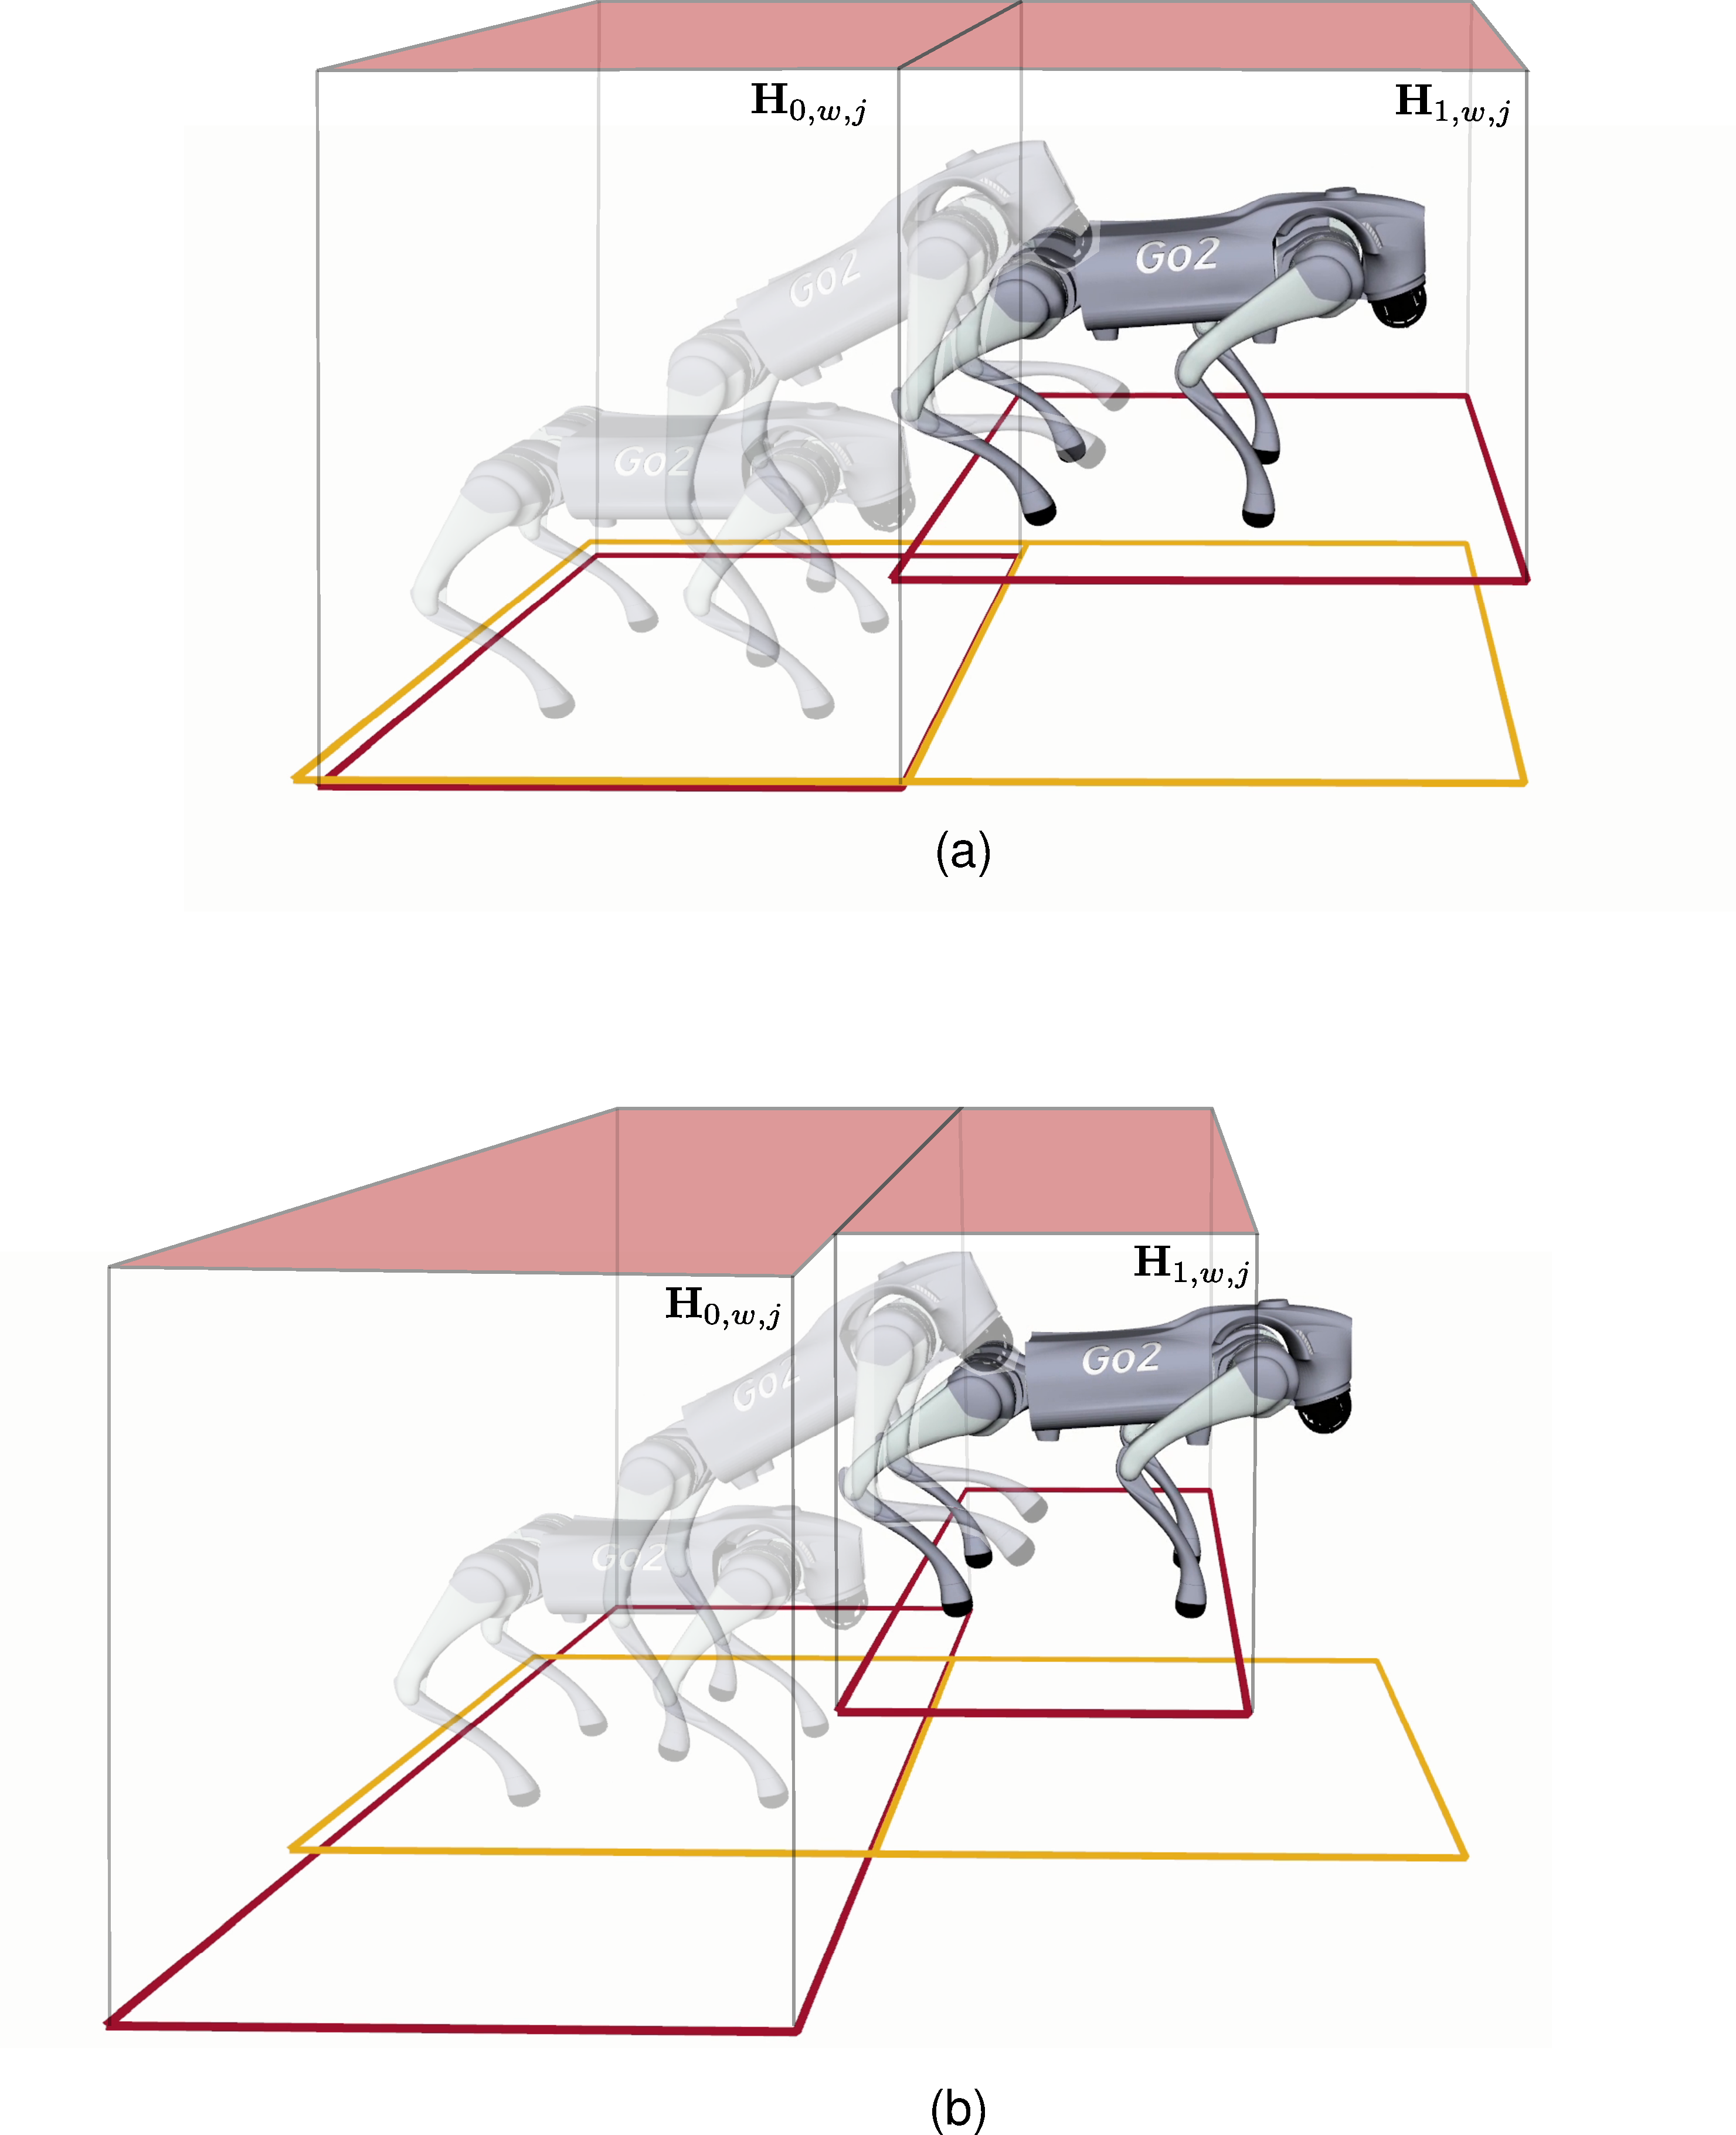
\includegraphics[width=\linewidth]{online_micp.pdf}
    \caption{Demonstrations of (a) offline MICP for a skill transitioning from a flat terrain to a high terrain with predefined polygons; (b) online MICP for the same skill but with online terrain polygons.}
    \label{fig:online_micp}
\end{figure}


\subsubsection{Robot Pose Re-Targeting}
Since the final targeting condition significantly influences the reference trajectory and the feasibility of the MICP problem, we evaluate the final condition by solving a kinematic feasibility problem (a simplified MICP in Eq.~(\ref{ocp:mip_general})) before solving the online MICP. Compared with the gait-fixed MICP, the dynamics equation (\ref{eq:dynamics}) is replaced by enforcing the center of mass (CoM) to lie inside a convex support polygon with all feet in stance to ensure static stability. In addition, a hard constraint is added to ensure that the modified robot pose stays within a certain threshold compared with the original desired pose. The cost function is simplified to stay as close as possible to the original desired pose. The higher-order terms of body position, orientation, and end-effectors are excluded from the decision variables. All the other constraints not involving those higher-order terms remain the same. Once the kinematic feasibility problem is solved successfully, the online MICP is solved using the modified re-targeted final condition and reference trajectory.

\subsubsection{Collision Avoidance and Swing Foot Constraints}
\revised{Our framework handles obstacles at \emph{two distinct levels}, and we will explicitly elaborate which level is responsible in which scenario.
\begin{itemize}
    \item \emph{Symbolic-level obstacle avoidance.} When an obstacle is large enough that an entire abstracted cell becomes unsteppable, it is classified as the \textit{obstacle} terrain class in the local symbolic abstraction (Sec.~\ref{sec:preliminaries_abstraction}). The symbolic specification rules out transitions into such cells, and if an obstacle appears at runtime---as in the rebar-with-obstacle hardware experiment, where the obstacle is detected via motion capture and added to the local abstraction online---runtime symbolic re-synthesis (Sec.~\ref{sec:online_repair}) finds a detour around it. No collision-region variables need to be added to the online MICP in this case.
    \item \emph{MICP-level collision-free region selection (this subsection).} For smaller obstacles that the swing foot must clear within a single symbolic transition, we encode collision avoidance directly in the online MICP. Because the resulting trajectory is sent directly to the tracking controller, the quality of end-effector (EE) trajectories at this layer is critical for tracking performance. We introduce binary variables $\v H_{s,w,j}$ that constrain the swing-foot trajectory of foot $j$ to lie inside one of $S$ pre-labeled collision-free convex polytopes at each time step. These free-space polytopes come from the same labeled-polygon segmentation pipeline as the steppable terrain, with a separate label set distinguishing free-space polytopes from steppable terrain polygons. In simulation, this mechanism is exercised in the \textit{Unstructured--8} case with collision avoidance enabled (see Table~\ref{tab:micp_speed}), where the binary-variable count rises to 256.
\end{itemize}
We do not perform full-body, mesh-level collision checking against arbitrary geometry; the body footprint is implicitly handled by steppable-region selection keeping each foot inside a labeled terrain polygon. The formulation here trades fidelity for online tractability.}

Specifically, $s \in \range{S}$ represents the $s^{\rm th}$ convex collison-free region and $w \in \range{W}$ denotes the $w^{\rm th}$ time step, evenly discretized with $\Delta t_w$ over the entire $W$ time steps. Fig.~\ref{fig:online_micp}(b) demonstrates two collision-free regions.
\begin{align}
    \nonumber & \forall s \in [S], w \in [W], j \in [n_f]\\\label{eq:collision_avoidance} &\v H_{s,w,j} \Rightarrow \v A_s \v p_j[i] \leq \v b_s, \forall i \in \mathcal{C}_{w,w+1}
        \\&\sum_{s=0}^{S-1}\v H_{s,w,j} = 1
        \\&\v H_{s,w,j} \in \{0, 1\}
\end{align}
where $\mathcal{C}_{w,w+1}$ denotes the set of continuous time steps that span from the $w^{\rm th}$ to the ${w+1}^{\rm th}$ binary time step. \revised{We emphasize that the collision-free region selection in Eq.~(\ref{eq:collision_avoidance}) and the steppable-region selection in Eq.~(\ref{eq:safe_region}) handle different geometric primitives: the steppable-region constraint forces \emph{stance-foot} placement onto a labeled steppable terrain polygon at the first stance time step, while the collision-free region constraint here keeps the \emph{swing-foot} trajectory inside a free-space polytope across all time steps within a swing phase. The two are complementary and not redundant.}

To enable larger swing foot clearance from the terrain, we also add constraints to force the swing foot height above a user-defined threshold $h_{\text{swing}}$, given the fixed contact timing. \revised{This constraint targets cleanly clearing the terrain during a transition---for example, when jumping onto a higher platform. While such clearance could in principle be enforced through the collision-free region selection alone, doing so would require a fine time-step discretization of the binary variables and would tend to yield trajectories that only marginally clear the terrain. The height threshold $h_{\text{swing}}$ instead provides a direct, continuously enforced clearance margin that is straightforward to tune.}

\revised{Note that the collision-avoidance and swing-foot constraints are also incorporated in the offline MICP as part of the feasibility-checking rules for the relevant terrain transitions. We highlight them here because their impact on online tracking performance is substantially more critical.}
% \begin{align}
%     &\v p_{j}^z[\text{mid}] \geq \v p_{j}^z[\text{start}] + h_{\text{swing}}\\
%     &\v p_{j}^z[\text{mid}] \geq \v p_{j}^z[\text{end}] + h_{\text{swing}}
% \end{align}
% where $\v p_{j}^z[\text{start}], \v p_{j}^z[\text{mid}], \v p_{j}^z[\text{end}]$ stand for the $j^{\rm th}$ EE positions in the z dimension at the starting, middle, and ending knot point of a swing phase, respectively. 

% \revised{Compared to the conference version~\citep{zhou2025physically}, the binary collision-region variables $\v H_{s,w,j}$, the swing-foot height parameterization, and their joint use in the online MICP are introduced in this article; the underlying gait-fixed MICP structure is shared with the conference version.}

% \begin{algorithm}[h!]\label{code:strategy_execution}
%   \caption{Strategy Execution}
%   \SetAlgoLined
%   \SetKwInOut{Input}{input}\SetKwInOut{Output}{output}
%   \PrintSemicolon
%    \Input{synthesized strategy $\mathcal{A}$, initial robot state $\v x_0$}
%    \Output{referenceTraj, gaitSequence}
%    \nl$\rm curNode$ = initializeNode($\v x_0$)\;
%     \nl\While{1}{
%         \texttt{// Roll out the automaton}\;
%         \nl\If{\rm previousWaypointReached}{
%         \texttt{// Check if local waypoint is changed}\;
%         \nl\If{\rm{!waypointPending} \& \textcolor{blue}{ \rm{localWaypointChanged}}}{
%             setNewWaypoint($\mathcal{X}_{\rm cen}^{\rm des}$, $\rm curNode$, $\mathcal{J}$)\;
%         }
%         \texttt{// Check if local terrain is changed}\;
%         \nl\If{\textcolor{blue}{\rm terrainStateChanged}}{
%             setUpdatedTerrain($\mathcal{E}$, $\rm curNode$, $\mathcal{J}$)\;
%         }
%         \texttt{// Find the next node and solve OCP}\;
%         \nl$\rm{nextNode}$ = findNextAllowableNode($\rm curNode$, $\mathcal{J}$)\;
%         \texttt{// Check goal pose feasibility}\;
%         \nl$\v x_{\rm init}$ = $\rm{referenceTraj}[-1]$\;
%         \nl($\rm goalFeasible$, $\v x_{\rm goal}$) = \textcolor{blue}{ solveInstantaneousOCP}($\rm nextNode$)\;
%         \nl\eIf{\rm goalFeasible}
%         {
%             \nl($\rm OCPsuccess$, $\rm traj$, $\rm gait$) = \textcolor{blue}{solveOCP($\rm curNode$, $\rm nextNode$)\;}}
%         {
%             \nl \textcolor{blue}{triggerReplan}\;
%         }
        
%         \nl\eIf{\rm OCPsuccess}{
%             \nl$\rm referenceTraj$ += $\rm traj$\;
%             \nl$\rm gaitSequence$ += $\rm gait$\;
%         }{
%             \nl \textcolor{blue}{triggerReplan}\;
%         }
%         \texttt{// Publish reference trajectory and gait}\;
%         \nl\If{$\mathcal{X}_{\rm cen} = \mathcal{X}_{\rm cen}^{\rm des}$}{
%             \nl publishReference($\rm referenceTraj$, $\rm gaitSequence$)\;
%             \nl clearReferenceTrajAndGait()\;
%             \nl \textcolor{blue}{requestReset}\;
%         }
%         \nl$\rm curNode$ = $\rm nextNode$\;
%         }
%         $\texttt{// Reset the current node}$\;
%         \nl\If{\rm resetRequested \& \rm{goalReached}} {
%             \nl$\rm curNode$ = findNodeAfterReset($\mathcal{E}$, $\rm curNode$, $\mathcal{J}$)\;
%         }
%     }
% \end{algorithm}

% \subsection{Online Repair}\label{sec:online_repair}
% During online execution, 
% the robot may encounter unexpected terrain states
% that the initial model of the workspace structure does not take into consideration.
% We leverage an online repair tool~\citep{meng2024automated} 
% to detect and recover from such unexpected terrain states.

% The online repair tool first generates a monitor that detects violations of the environment assumptions $\envsafety$ during online execution.
% %
% Note that $\envsafety$ includes the assumption
% $\envterrain = $ $
%     \square (
%     \bigvee_{\statevar\in\inpstateterrainposs}
%     \form{\inpterrain}{\statevar})$,
% which assumes that 
% at any time, 
% at least one terrain state from the set of possible terrain states $\inpstateterrainposs$ must hold
% % the current terrain state $\inpstateterrain$
% % must always come from
% % $\inpstateterrainposs$, 
% % the set of possible terrain states provided by the user
% (see Sec.~\ref{sec:spec_gen}).
% % Suppose the current terrain state $\inpstateterrain$ is not in $\inpstateterrainposs$, the set of possible terrain states provided by the user.
% During online execution,
% if the current terrain state $\inpstateterrain \not\in \inpstateterrainposs$,
% the monitor detects that $\inpstateterrain$
% violates the assumption $\envterrain$.
% We then relax the violated assumption $\envterrain$ to admit the new terrain state $\inpstateterrain$,
% replacing $\envterrain$ with 
% $\square (
%     \bigvee_{\statevar\in\inpstateterrainposs\cup\{\inpstateterrain\}}
%     \form{\inpterrain}{\statevar})$.
% After assumption relaxation,
% the revised specification becomes unrealizable
% as the robot lacks the required skills to handle the new terrain state $\inpstateterrain$.
% We utilize symbolic repair 
% (Sec.~\ref{sec:symbolic_repair})
% to find a set of necessary skills for the new terrain state.
\subsection{Runtime Repair}\label{sec:online_repair}
% The runtime repair takes in
% a terrain state $\inpstateterrain \in \inpstatesterrain$, 
% a request state $\inpstaterequest \in \inpstatesrequest$,
% and a Boolean formula $\disallowedtrans$
% representing disallowed transitions discovered at runtime.
% We first update the system hard constraint $\syssafety$ in the specification $\spec$ from Sec.~\ref{sec:spec_gen}
% to be $\syssafety \land \square \disallowedtrans$,
% so that the updated specification respects the newly discovered disallowed transitions, if any.
% We then
% leverage the high-level manager to create a partial evaluation of $\spec$ over $\inpstateterrain$ and $\inpstaterequest$,
% and perform symbolic repair 
% to generate new robot skills and a new strategy to handle $\inpstateterrain$ and $\inpstaterequest$,
% as done in Sec.~\ref{sec:manager_and_repair}.
The runtime repair procedure takes as input a terrain state $\inpstateterrain \in \inpstatesterrain$, a request state $\inpstaterequest \in \inpstatesrequest$, and a Boolean formula $\disallowedtrans$ that encodes disallowed transitions identified at runtime. We first update the system’s hard constraint $\syssafety$ in the specification $\spec$ (see Sec.~\ref{sec:spec_gen}) to $\syssafety \land \square \disallowedtrans$, ensuring that the specification reflects these newly discovered restrictions. Next, the high-level manager constructs a partial evaluation of $\spec$ over $\inpstateterrain$ and $\inpstaterequest$. Symbolic repair is then applied to generate additional robot skills and synthesize a new strategy that accommodates the current terrain and request states, following the approach in Sec.~\ref{sec:manager_and_repair}.





% the prior knowledge of the workspace structure does not take into account.
% \begin{enumerate}
%     \item Encounter unexpected terrain states during execution
%     \item Generate a monitor to check assumption violations
%     \item The monitor detects that the new terrain state violates the environment assumption which states that the current terrain state must belong to the set of possible terrain states.
%     \item we relax the assumption to include the new terrain state
%     \item we perform repair obtain new skills that can handle the new terrain state, and resume the execution
% \end{enumerate}


\section{Tracking Control}\label{sec:tracking_control}
The tracking control module adopts an MPC-Whole-Body-Control (WBC) hierarchy, ensuring precise end-effector (EE) and centroidal momentum tracking. To smoothly and efficiently execute the strategy considering the potential computational delay in solving MICP, a harmonic coordination module between the strategy automaton roll-out and the tracking module is designed (Sec.~\ref{sec:coordination}).

\subsection{Tracking Control Module}
\subsubsection{Nonlinear Model Predictive Control (NMPC)}\label{subsec:nmpc}
The NMPC  operates independently from the symbolic planning module, tracking reference trajectories generated by the online MICP using a more accurate dynamics model. In this work, the NMPC accounts for the robot's centroidal dynamics and kinematics, similar to approaches in \citep{dai2014whole,chignoli2021humanoid,sleiman2021unified}, presenting a more accurate model than the simplified angular dynamics in the MICP. An analytical inverse kinematics solution based on the MICP output provides the full joint state reference trajectory for the NMPC.
In addition to standard frictional and contact constraints and base tracking costs, an additional cost function for EE reference tracking from the MICP is included to enhance precision. The NMPC optimization problem is formulated as a Sequential Quadratic Program (SQP) and solved using the OCS2 library \citep{OCS2}, with a time horizon of one second and 100 knot points.

\subsubsection{Whole-Body Control (WBC)}
While NMPC operates at the centroidal level to generate dynamically feasible trajectories, WBC ensures precise execution by resolving full-body state control, including joint torques, accelerations, and contact forces.
The whole-body controller tracks the NMPC trajectory by solving a weighted quadratic program (QP) \citep{kuindersma2014efficiently} at 500 Hz. To improve the performance of agile motions such as leaping and jumping, centroidal momentum tracking \citep{wensing2013generation} is included. This MPC-WBC hierarchy allows the system to handle both centroidal-dynamics-level and full-body-dynamics-level control in a coordinated manner, ensuring robustness in real-world deployment especially for highly dynamic motions such as jumping.

\subsubsection{State Estimation}
The state estimator employs a linear Kalman filter similar to that in \citep{bledt2018cheetah}, with the addition of OptiTrack motion capture (mocap) measurements fused alongside IMU data and joint encoder readings to achieve accurate body position estimation. For agile motions such as jumping, we observed improved base-height estimation by assigning higher noise values to the mocap feedback during aerial phases, due to its limited 120 Hz update rate.
\subsection{Coordination between Strategy Execution and Tracking Module}\label{sec:coordination}
\begin{figure}
    \centering 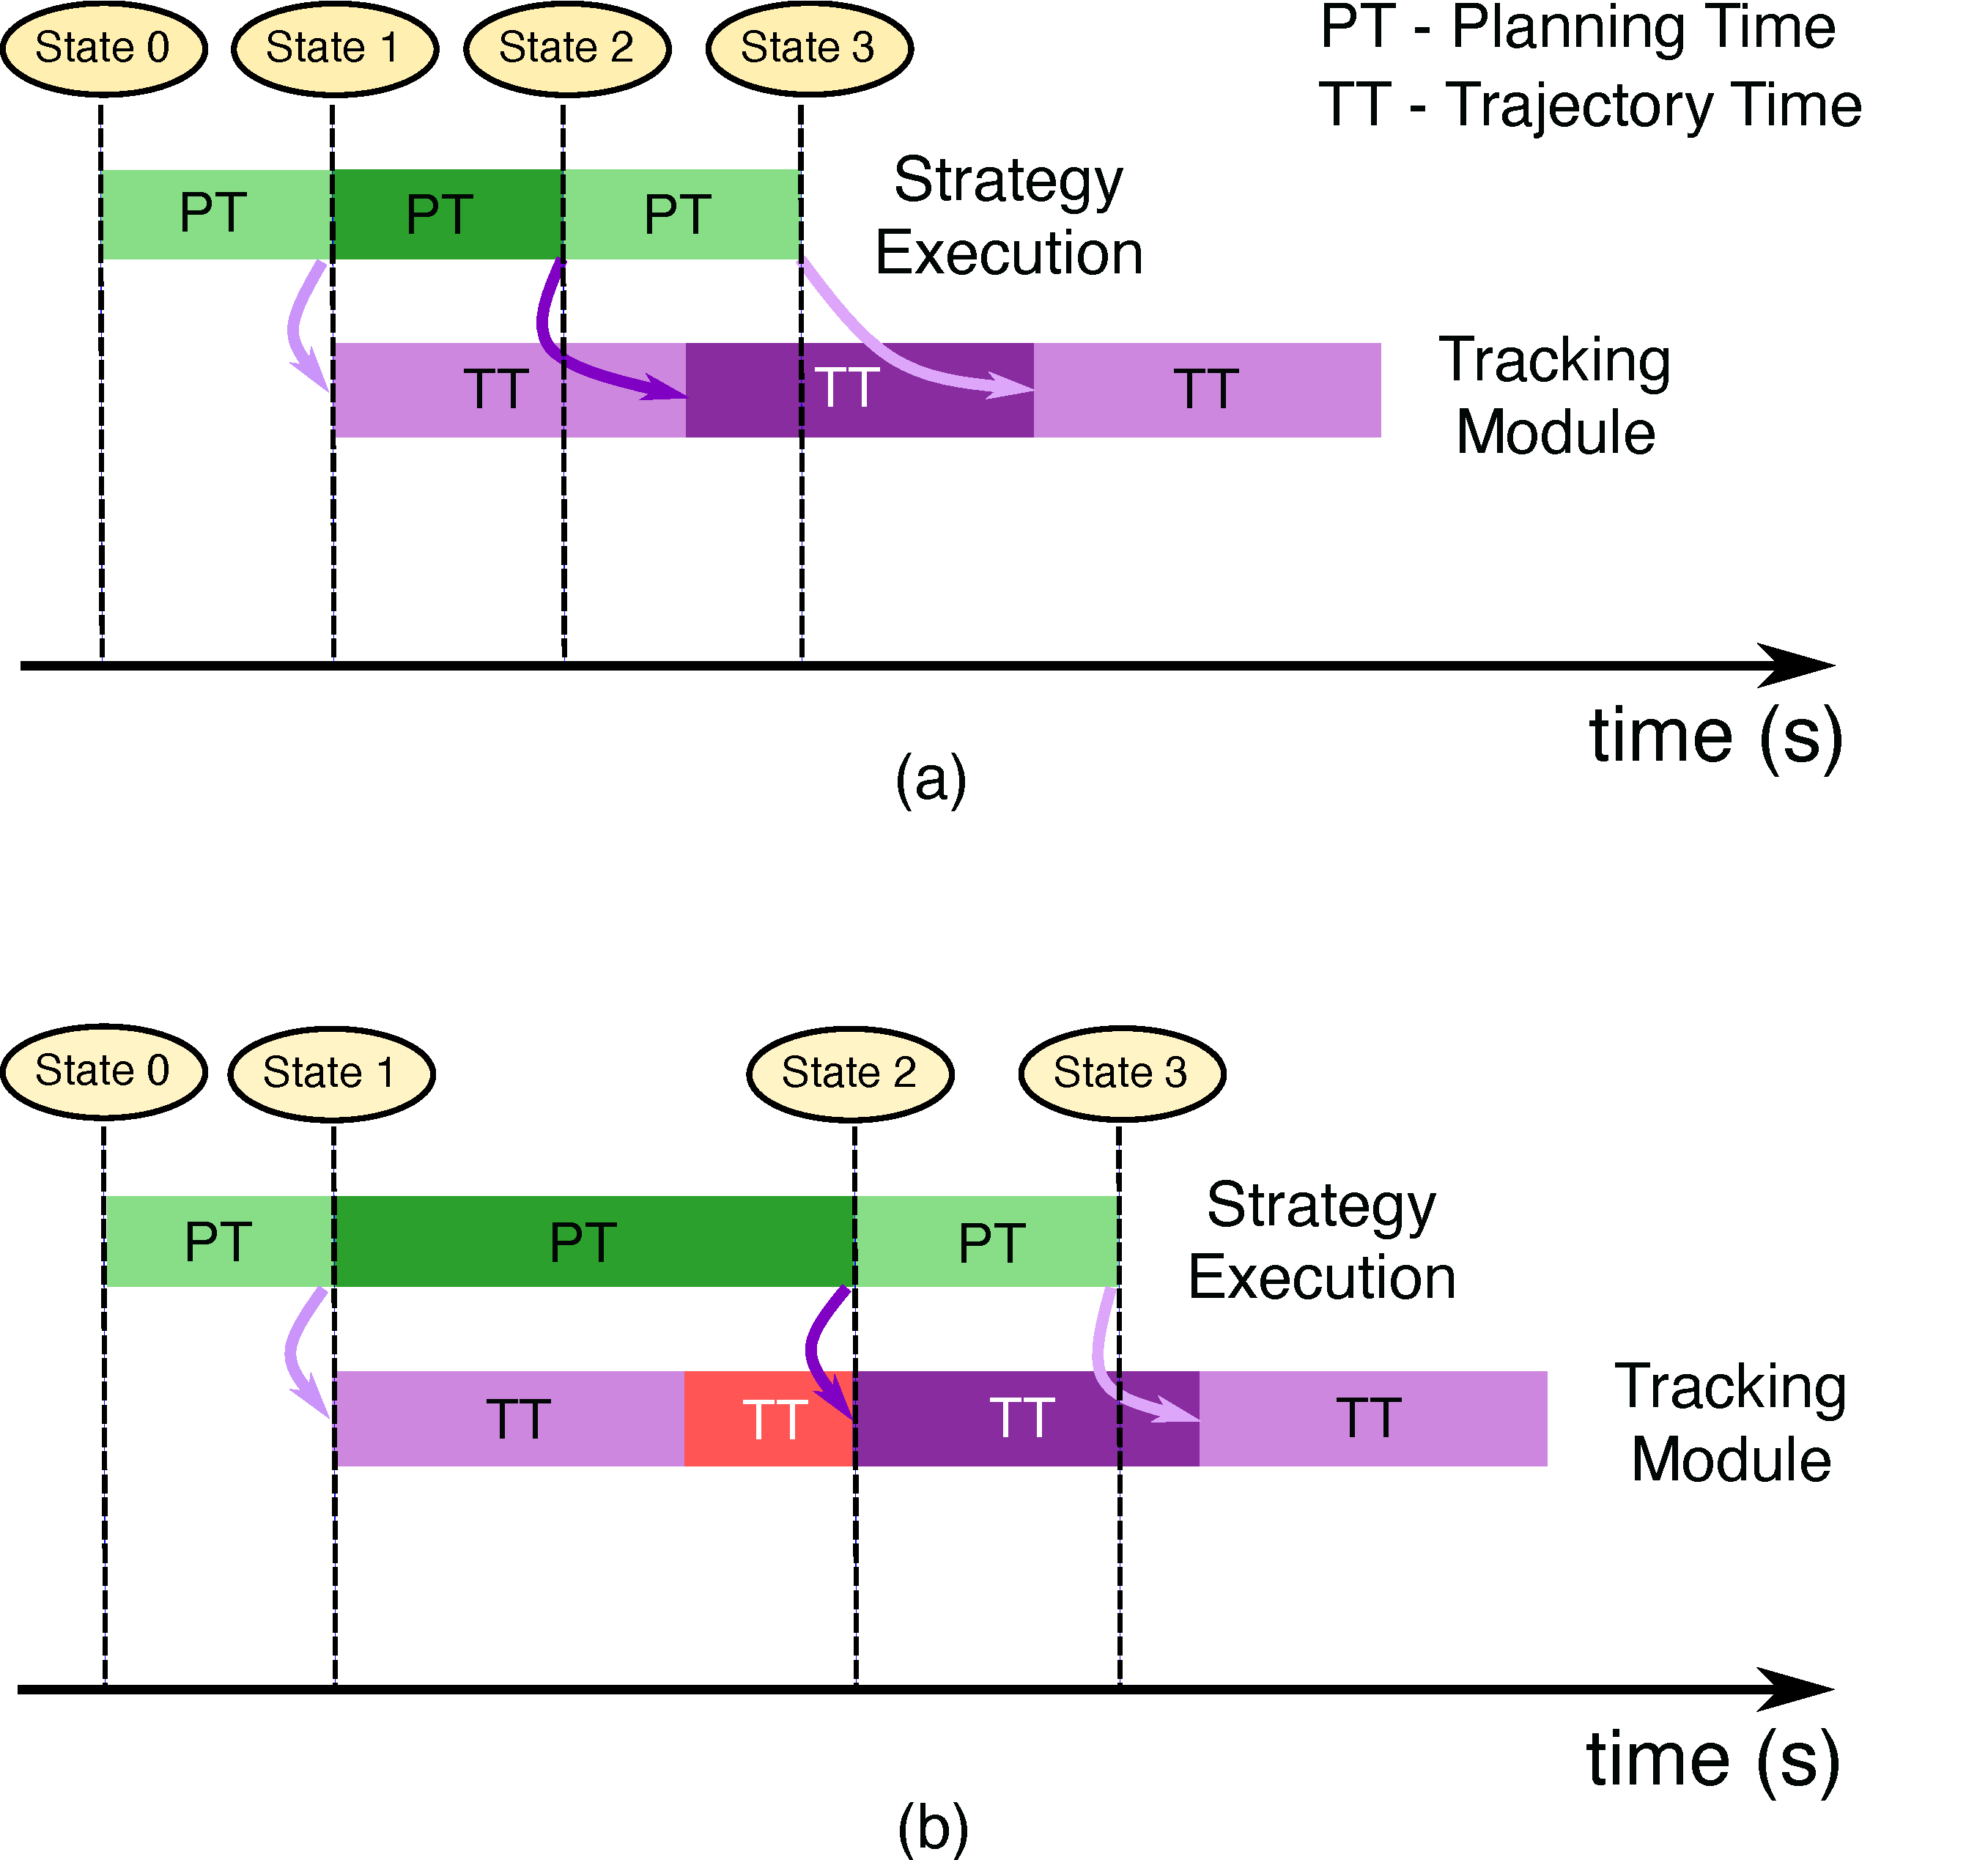
\includegraphics[width=\linewidth]{multi_threading_new.pdf}
    \caption{Coordination between strategy execution and tracking control module.
    (a) The MICP solving time (denoted by PT) for transitioning from State 1 to State 2 is shorter than the time horizon of the previous reference trajectory (denoted by TT), allowing the seamless appending for the new trajectory.
    (b) The MICP solving time exceeds the time horizon of the previous reference trajectory, requiring the robot to come to a stop (red) and wait for the new trajectory whenever available.}
    \label{fig:micp_mpc_automaton}
\end{figure}
Due to the potential delays in solving MICP during the strategy automaton roll-out, a harmonic coordination between the strategy execution and tracking control module is essential. The tracking module's reference trajectory is updated dynamically alongside the strategy execution process, as shown in Fig.~\ref{fig:micp_mpc_automaton}. The overall process can be summarized as follows:

\subsubsection{Strategy Execution} The strategy automaton execution thread begins by solving the online gait-fixed MICP, starting from State 0 in the automaton. Once the MICP solution is obtained, it immediately sends the reference trajectories and corresponding contact information to the tracking control module. The automaton then progresses to the next transition, using the final condition in the previous trajectory segment as the new initial condition. In Fig.~\ref{fig:micp_mpc_automaton}, the colored blocks in the strategy execution timeline indicate the time taken for each MICP solve during the automaton roll-out. PT and TT denote the planning time and trajectory time, respectively.

\subsubsection{Tracking Control Module}
The MPC-WBC tracking control module receives time-indexed reference trajectories, which can be updated in real-time. After completing the tracking of the current reference trajectory, the robot returns to a stance phase, ready to accept new reference trajectories. As depicted in Fig.~\ref{fig:micp_mpc_automaton}, the colored blocks in the tracking control module represent the time horizon of each reference trajectory sent by the strategy execution thread. Once the initial reference trajectory is generated, the MPC-WBC thread begins tracking it using more accurate dynamics models, as described in Sec.\ref{sec:tracking_control}.

\subsubsection{Delay Handling}
For more complex scenarios involving a larger number of terrain polygons, the MICP solving time may increase and exceed the time horizon of the generated reference trajectory. Fig.~\ref{fig:micp_mpc_automaton}(a) and (b) illustrate two cases of MICP solving times:
Case (a): The solving time for transitioning from automaton State 1 to State 2 is shorter than the time horizon of the previous reference trajectory. In this case, the new reference trajectory is seamlessly appended to the existing one, and the robot continues tracking the previous trajectory.
Case (b): The solving time exceeds the time horizon of the previous reference trajectory, and the robot has already entered a stance phase (red block) when the MICP solution is obtained. In this case, the robot waits until the newly generated reference trajectory is sent based on the current system time (red block in Fig.~\ref{fig:micp_mpc_automaton} (b)).

% \subsubsection{Error Handling and Replanning}
% If the MPC thread predicts a state that reaches the final state but deviates beyond the specified tolerance, the automaton thread resets to this new initial state and reruns the MICP to adjust the plan. If no significant deviation occurs, the automaton thread continues rolling out, using the desired state until the local waypoint is reached.



%%%%%%%%% Result %%%%%%%%
% \section{Offline Synthesis and Repair Case Study}
\begin{figure}
    \centering
    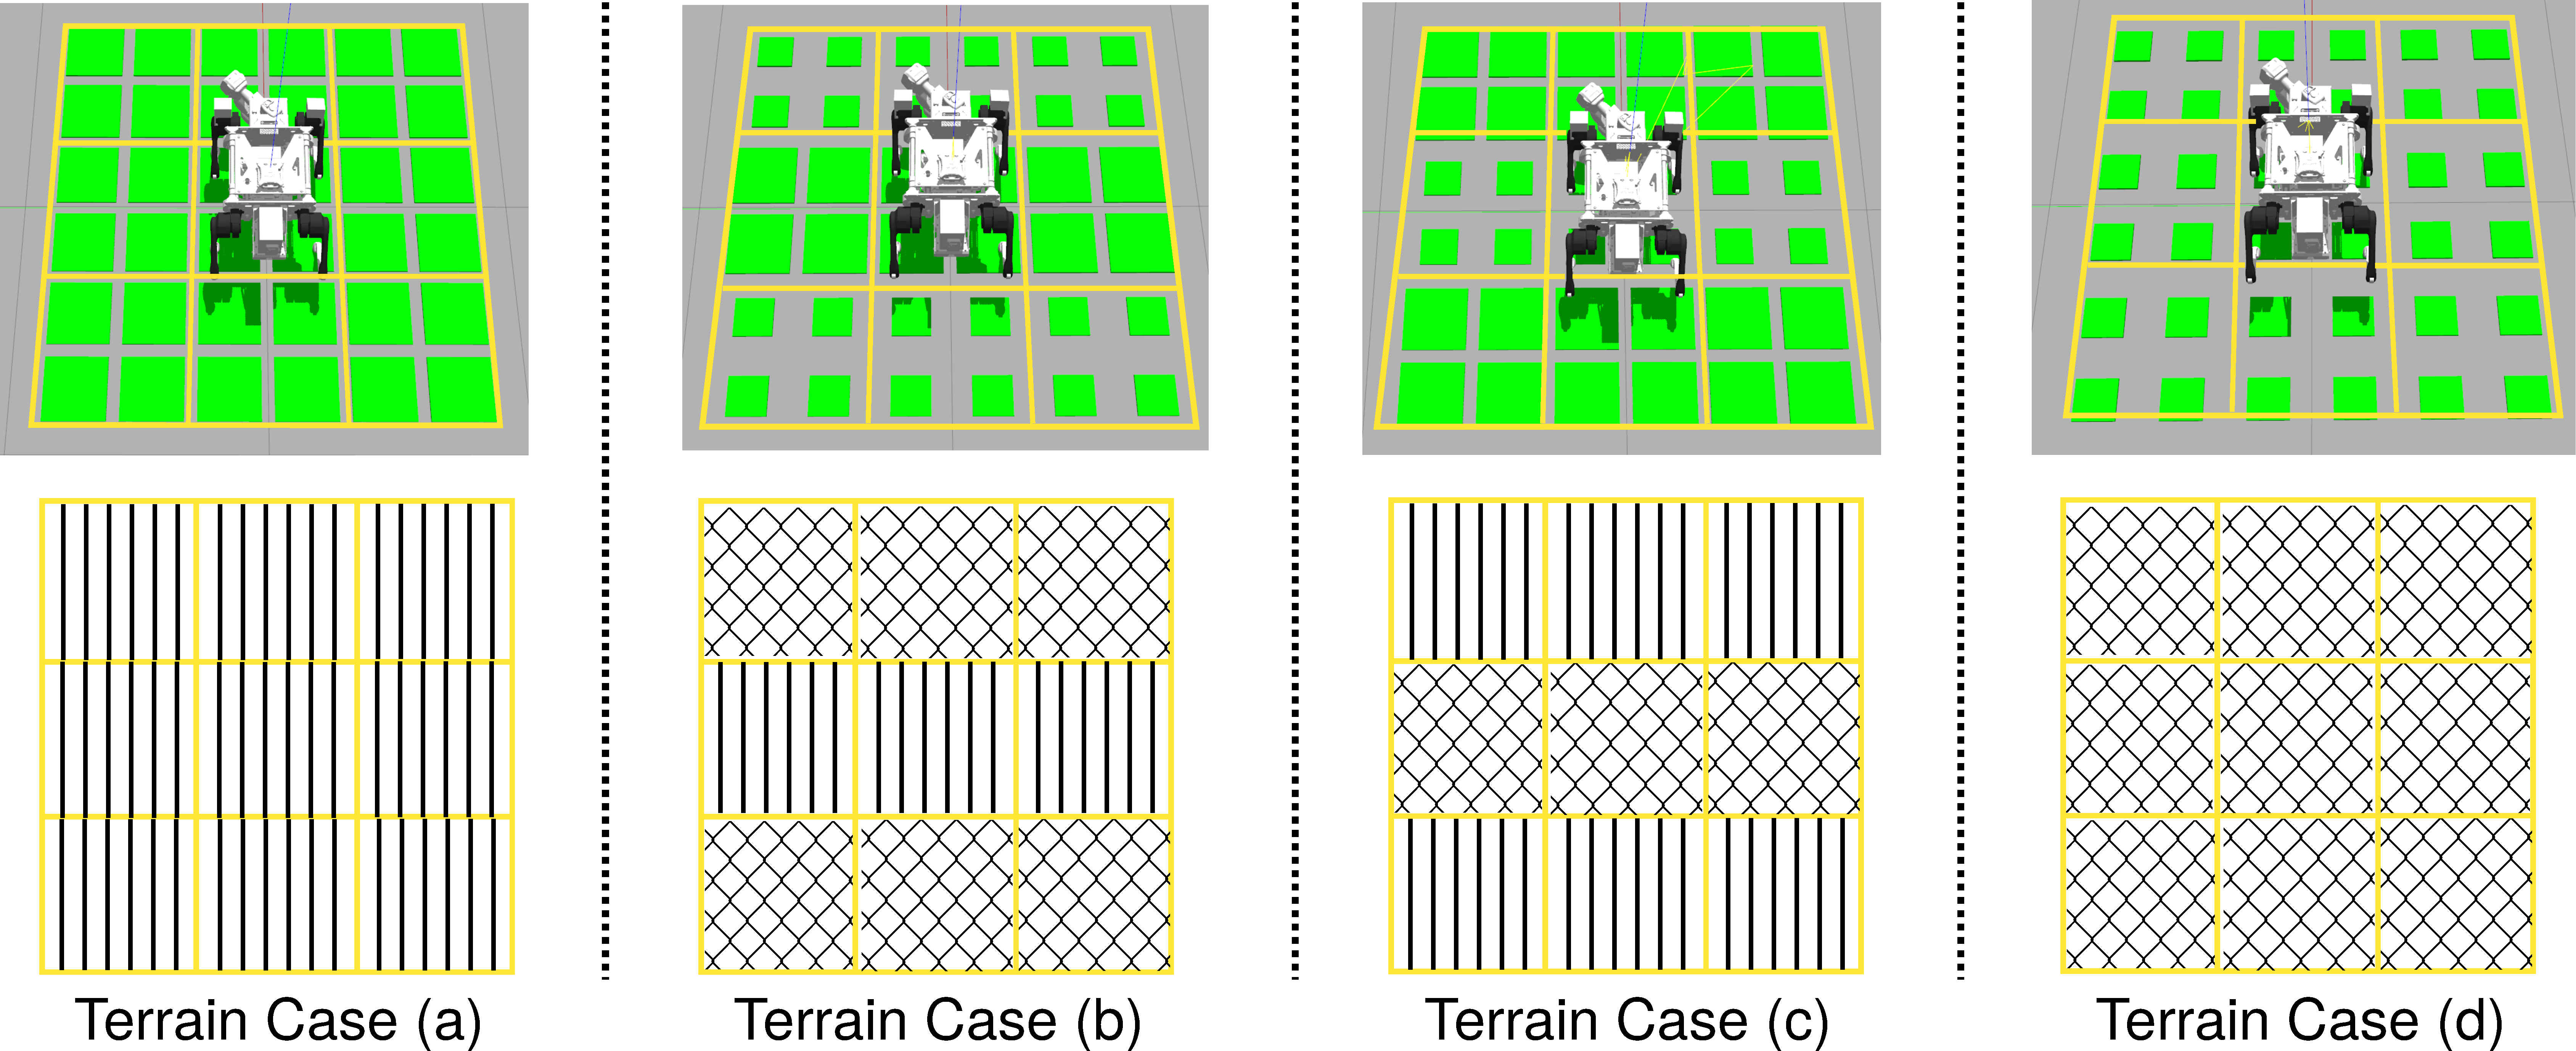
\includegraphics[width=1\linewidth]{offline_terrains.pdf}
    \caption{Four terrain cases used for offline repair in our case study.}
    \label{fig:offline_terrains}
\end{figure}
\begin{figure}
    \centering
    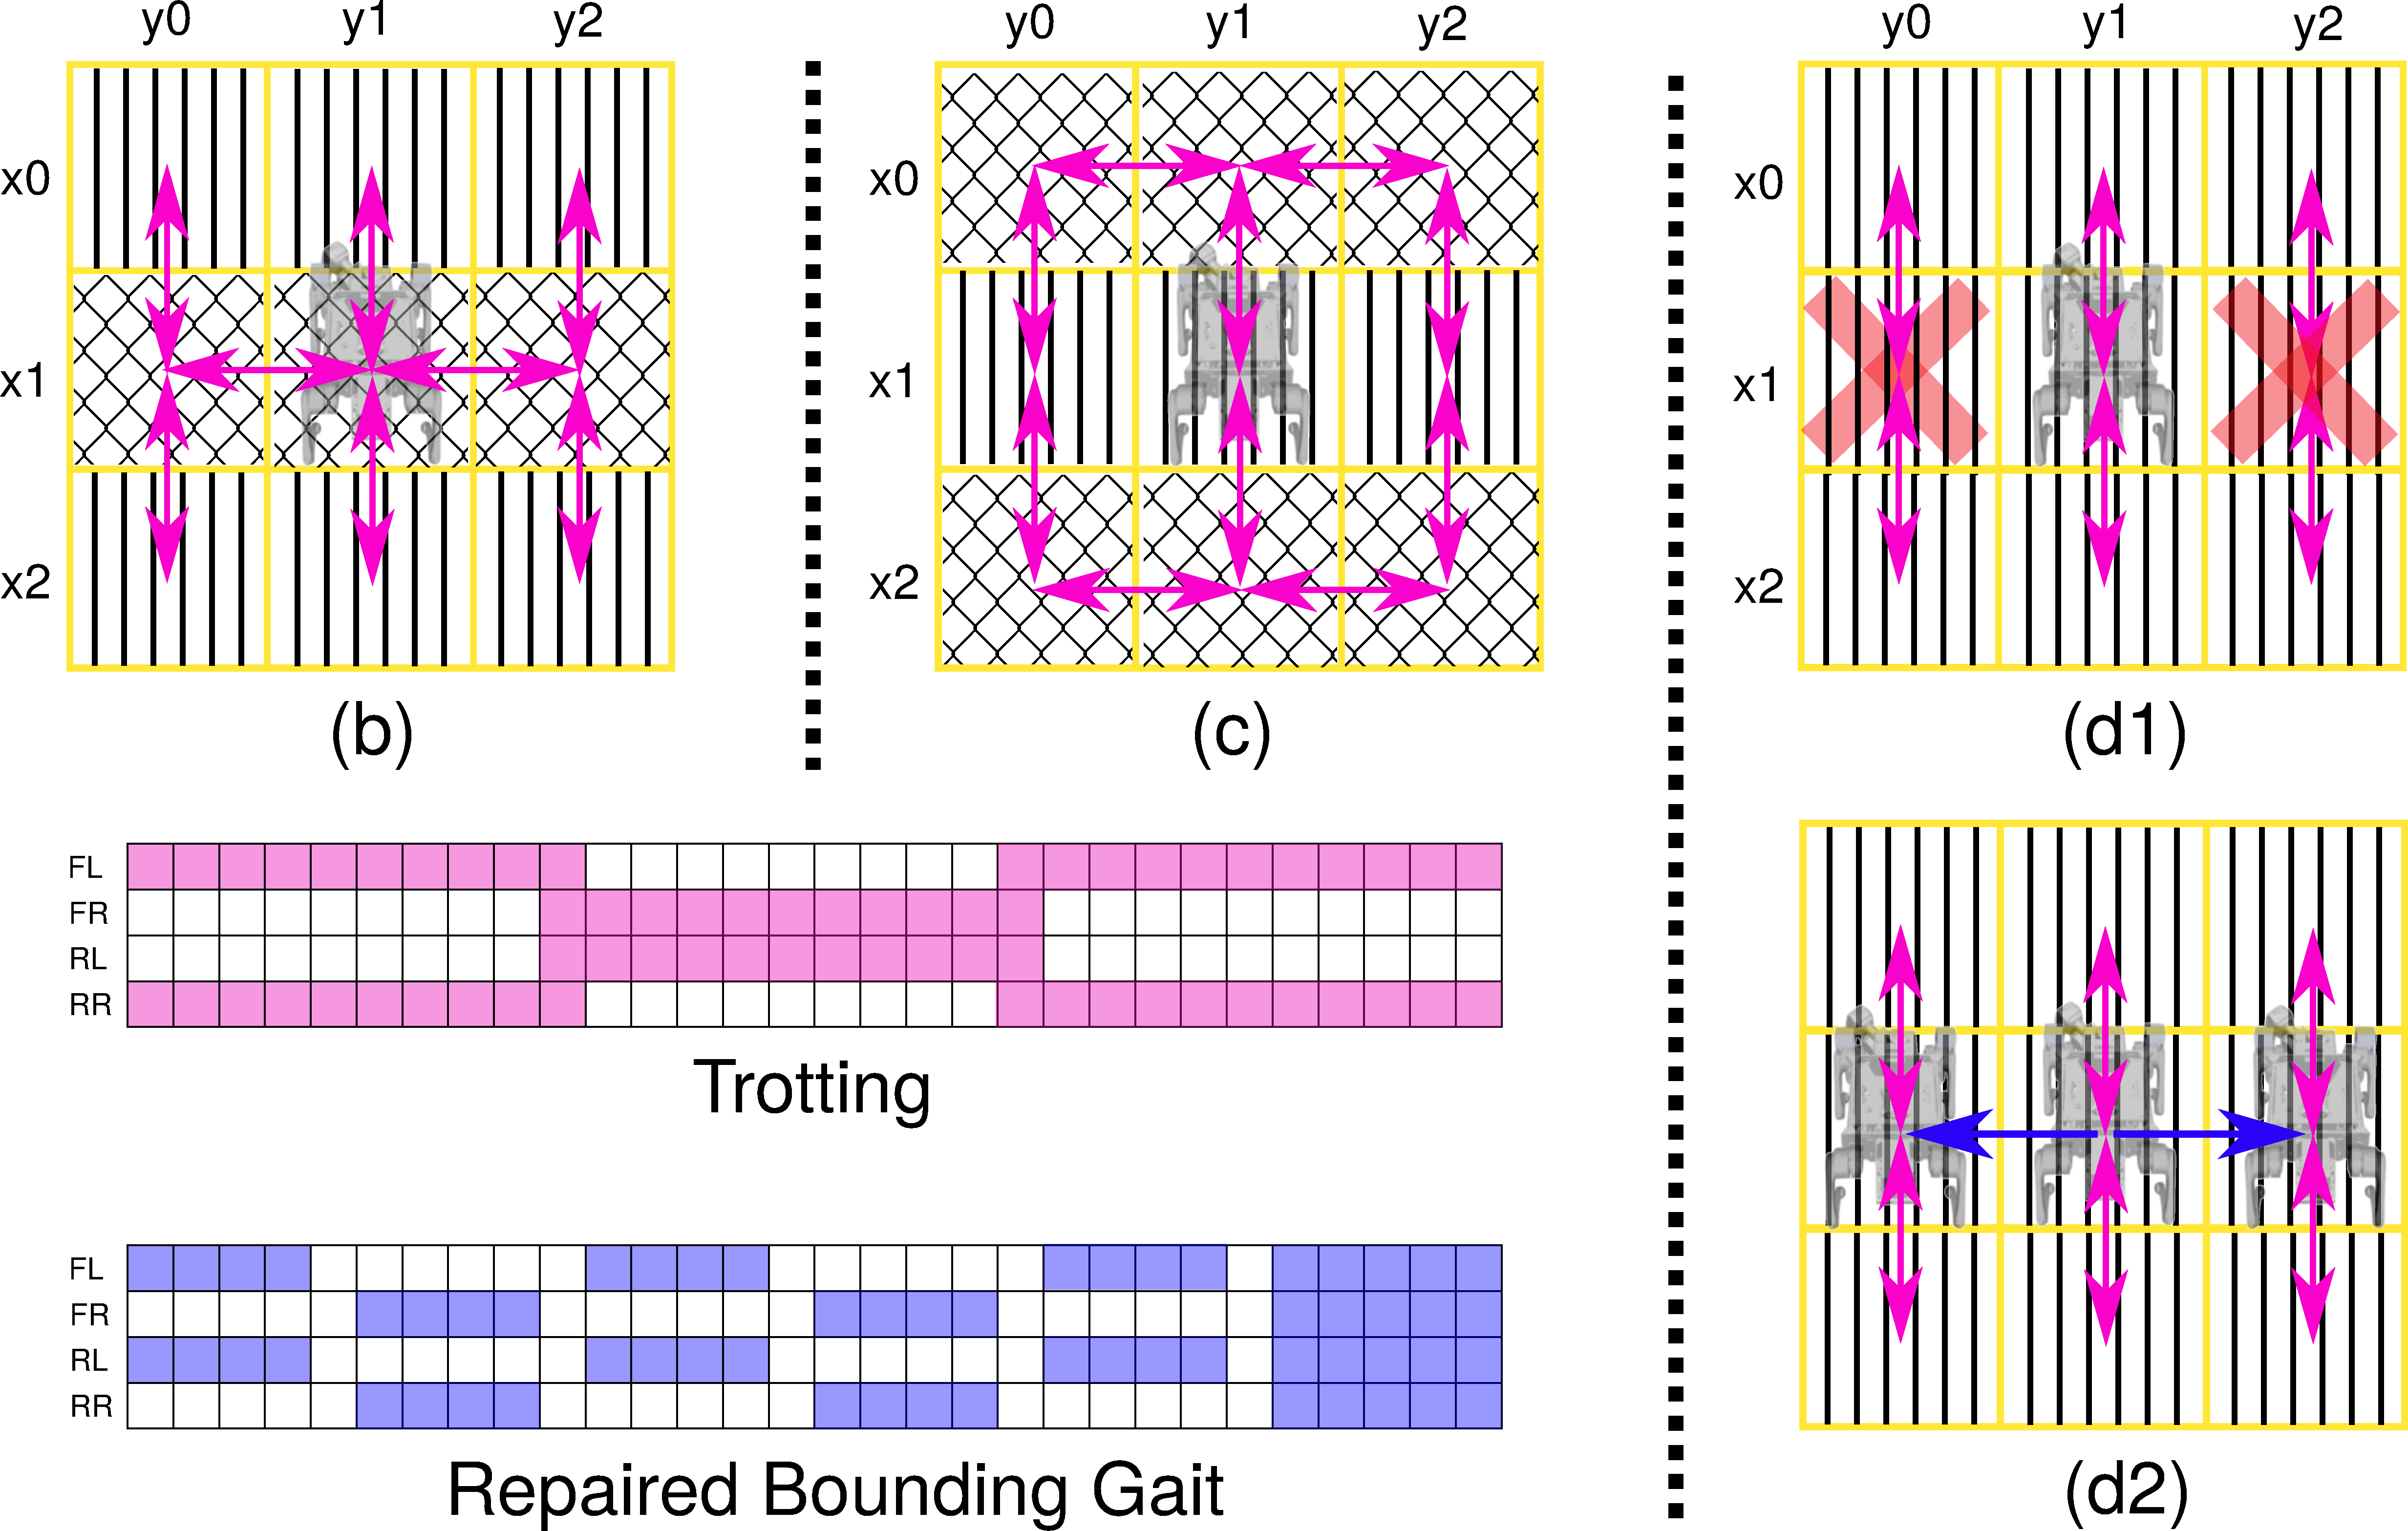
\includegraphics[width=\linewidth]{offline_repair.pdf}
    \caption{Offline repair results for terrain cases (b), (c), and (d) in Fig.~\ref{fig:offline_terrains}. We also illustrate the original trotting and repaired bounding gait.}
    \label{fig:offline_repair}
\end{figure}
We first present a case study to demonstrate the synthesis and repair processes in offline phase. 
% \subsection{Offline Synthesis and Repair Case Study}
Complementary to Example~\ref{example:1}, we provide additional set of predefined terrain polygons, which are abstracted into sparse and dense terrain types similar to Example~\ref{example:1}.
Fig.~\ref{fig:offline_terrains} shows four 9-grid terrain combinations with varying stepping stone sparsities. The first row presents the real-world terrain polygons, while the second row displays the corresponding symbolic-level maps. The grid size is chosen based on factors such as robot size and terrain dimensions. In this case study, we use a 0.6 m cell size and a $1.5$ s trotting gait as the motion primitive given ahead of time, and the MICP planner has a $0.02$ s timestep, resulting in $N=75$ knot points, and $R=8$ terrain polygons per transition. 

In Fig.~\ref{fig:offline_repair}, the pink arrows indicate the original feasible transitions after performing the gait-fixed MICP. The robot successfully navigates upward and downward across all terrains; terrain case (a) achieves all transitions and is not shown in the figure due to space limit. 
The infeasible transition arises when moving sideways on sparse stepping stones, restricted by the leg kinematics constraint in Eq.~\ref{eq:rom}. However, specifications for terrain case (b) and (c) remain realizable as the robot avoids sideways movement by taking detour steps, indicating that not all skills are required for these types of  terrains. Such a coincidence does not apply to terrain case (d), where the specification becomes unrealizable due to physically unreachable $(x_1,y_0)$ and $(x_1,y_2)$. This unrealizability triggers a symbolic repair to identify a symbolic suggestion, adding two additional transitions (blue arrows). By reconfiguring to a bounding gait with short aerial phases through gait-free MICP, the robot restores transition feasibility, making terrain case (d)'s specification realizable.

% we the offline terrains for specification generation. We use the above case for demonstrating the offline repair. We can emphasize that not all the transitions are needed for navigating to a desired waypoint considering the robot physical feasibility. The robot does not necessarily need to move sideways. It becomes more urgently needed when the state space increases. This also allows us to incorporate strategy in terms of specific terrain combinations. Only exception case is the one with all sparse terrains.



\section{Simulation}\label{sec:experiments}
We present examples of maneuvering across diverse environments in a Gazebo simulation to demonstrate the framework's efficacy, scalability, and generalizability.
In addition, benchmarking experiments are conducted to further compare our proposed framework with pure-MIP approaches.

\revised{\subsection{Implementation Details}\label{sec:impl_details}
All MICP problems---including the offline gait-free MICP, the online gait-fixed MICP, the kinematic-feasibility re-targeting MICP, and the pure-MIP benchmark---are solved using Gurobi~9~\citep{gurobi}. The NMPC tracker is implemented with the OCS2 library~\citep{OCS2}. All offline-synthesis, simulation, and online-planning experiments are run on a desktop workstation equipped with an Intel Core i9-13900K (24 cores) and 64\,GB of RAM. Reported solve times reflect this desktop-class CPU and should be interpreted as such; onboard, low-power deployment is left as future work.}

\subsection{Robot Setup}
As shown in Fig.~\ref{fig:hardware_info}, we verify our algorithms on two separate robot platforms, Unitree Go2 and SkyMul Chotu (a modified Unitree Go1 robot dedicated for rebar tying tasks). The SkyMul Chotu is equipped with a rebar gun mounted on its head and customized ``cross"-shaped feet designed for reliable standing on rebars. Note that in simulation, this foot shape is simplified to a regular round foot to avoid the complexity of simulating contact with irregular surfaces. In our planner, we model both cases as point contact.
The parameters for each robot are defined in Table~\ref{tab:robot_parameter} and used in our implementation, including the robot mass $m$, torque limit $\vg \tau_{\text{max}}$ and the reference joint position $\v q_j^{\text{ref}}$ for a single leg with three joints, the reference foot position relative to the base frame $^\mathcal{B} \v p_j^{\text{ref}}$ and the maximum deviation of the foot position $\v p_j^{\text{max}}$ for the front left leg ($j=0$), and the moment of inertia of the approximated single rigid body $\v I$.
\begin{figure}[t]
    \centering
    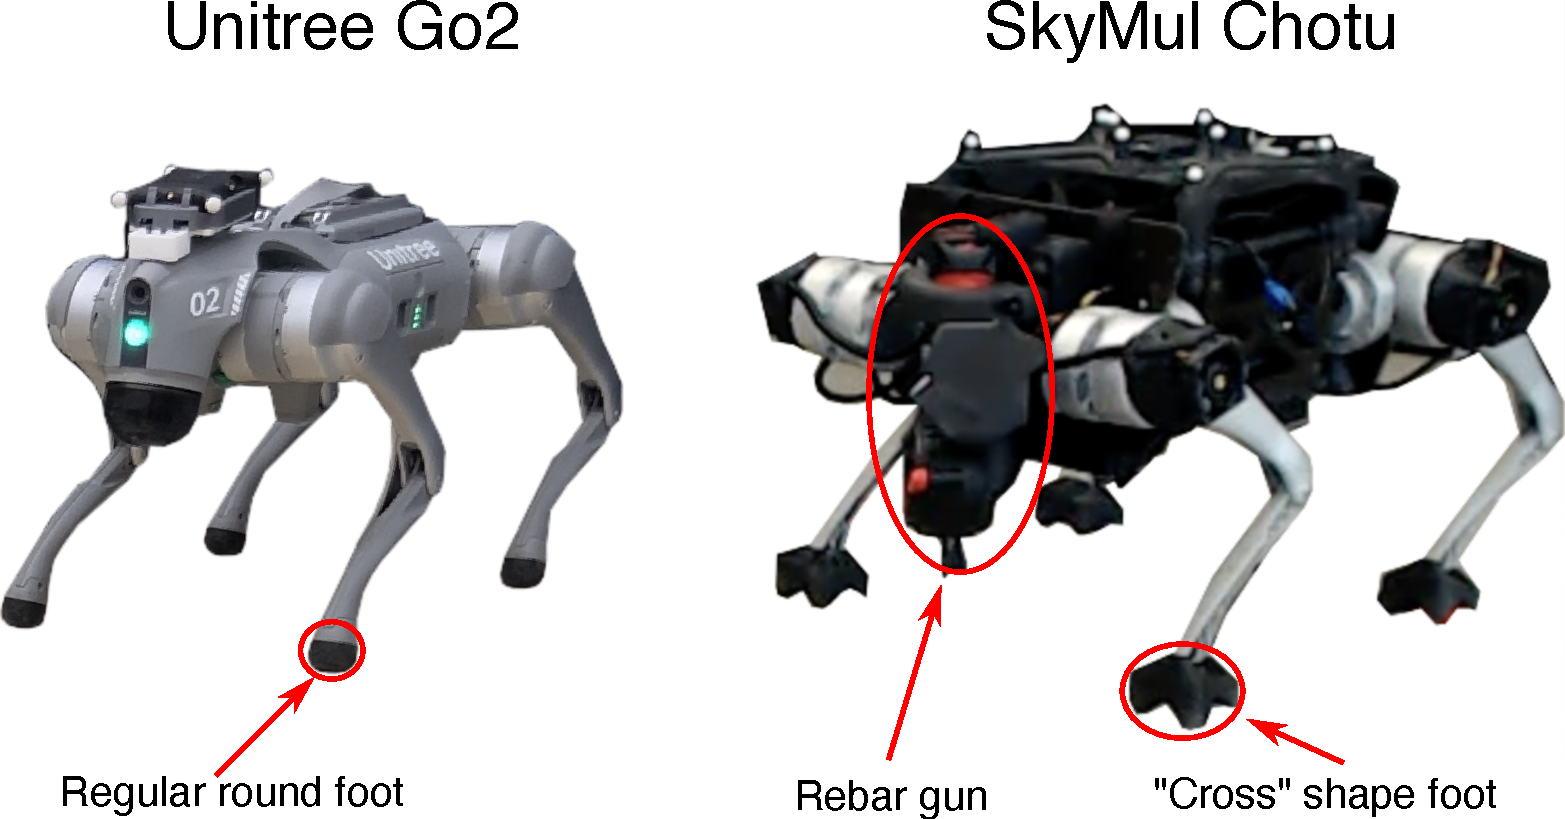
\includegraphics[width=0.85\linewidth]{hardware_info.pdf}
    \caption{Hardware platforms used for experiments: Unitree Go2 and SkyMul Chotu (equipped with a rebar gun and ``cross"-shaped feet).}
    \label{fig:hardware_info}
\end{figure}
\begin{table}[t]
\centering
\footnotesize
    \caption{Robot Parameters}
    \setlength{\tabcolsep}{4pt}
     \begin{tabular*}{\linewidth}{@{\extracolsep{\fill}}lll}
         \hline
         \textbf{Parameter} & \textbf{Unitree Go2} & \textbf{SkyMul Chotu}\\\hline
         $m$ (kg) & 15 & 20\\
         $\vg \tau_{\text{max}} $ (N $\cdot$ m) & (23.5, 23.5, 45.4) & (23.5, 23.5, 33.5)\\
         $\v q_j^{\text{ref}}$ (rad) & (0.0, 0.72, -1.44) & (0.0, 0.72, -1.44)\\
         $^\mathcal{B} \v p_j^{\text{ref}}$ (m) & (0.1805, 0.1308, -0.29) & (0.2118, 0.210, -0.30)\\
         $\v p_j^{\text{max}}$ (m) & (0.15, 0.1, 0.15) & (0.15, 0.1, 0.15)\\
         $\v I$ (kg $\cdot$ m$^2$) & diag(0.152, 0.369, 0.388) & diag(0.396, 0.915, 1.107)\\
         \hline
    \end{tabular*}
    \label{tab:robot_parameter}
\end{table}

% \todo Show the successful rate of navigation

\begin{figure*}[t!]
    \centering
    \includegraphics[width=\linewidth]{unstructured_and_rebar_maneuver_large.png}
    \caption{Snapshots from online execution across the four simulation scenarios: (a) unstructured terrain with four terrain types, (b) unstructured terrain with the full eight-type abstraction, (c) rebar terrain with the 7-type abstraction, and (d) rebar terrain with the 14-type abstraction. Green trajectories in (c) and (d) are detours produced by runtime re-synthesis after online MICP solving failures.}
    \label{fig:online_terrains}
\end{figure*}

\begin{table*}[t]
\centering
\footnotesize
    \caption{Offline Synthesis and Repair Time}
    \setlength{\tabcolsep}{4pt}
     \begin{tabular*}{\linewidth}{@{\extracolsep{\fill}}cccccc}
         \hline
         \textbf{Scenario} & \textbf{Grid Size} &
         % Terrain States $\times$ Request States
         \begin{tabular}{@{}c@{}}\textbf{Terrain and Request State Pairs}\\ \textbf{(Success/Total)}\end{tabular}
         & \begin{tabular}{@{}c@{}}\textbf{Number of Skills} \\ \textbf{(Original/New/Total)}\end{tabular} & \textbf{Symbolic Repair Time (s)} & \begin{tabular}{@{}c@{}}\textbf{Feasibility Check Time (s)}\\ \textbf{(Gait-Fixed/Gait-Free)}\end{tabular}\\\hline
         Unstructured - 4 & $3 \times 3$ & 169/169 & 18/\textcolor{red}{13}/64 & 8.07 &  18.97/449.94 \\
         & $5 \times 5$ & 129/158 & 19/\textcolor{red}{9}/64 & 77.16 &  20.26/241.42 \\\hline
         Unstructured - 8 & $3 \times 3$ & 250/264 & 19/\textcolor{red}{20}/256 & 14.90 & 22.92/382.63 \\
         & $5 \times 5$ & 179/246 & 20/\textcolor{red}{16}/256 & 93.21 & 18.59/196.88\\\hline
         Rebar - 7& $3 \times 3$ & 
         % -/258 & 47/-/52 & - &  116.69/- 
         196/196 & 18/\textcolor{red}{11}/196 & 7.44 &  15.63/417.55
         \\
         & $5 \times 5$ & 196/196 & 18/\textcolor{red}{10}/196 & 21.63 &  14.83/374.89 \\\hline
         Rebar - 14 & $3 \times 3$ & 237/237 & 20/\textcolor{red}{29}/784 & 10.34 & 21.92/701.38\\
         & $5 \times 5$ & 196/196 & 20/\textcolor{red}{18}/784 & 24.31 & 23.06/453.94 \\\hline
    \end{tabular*}
    \label{tab:offline_synthesis_time}
\end{table*}

\subsection{Simulation Environment Setup}
To demonstrate the generalizability of our proposed framework, we evaluate it across two scenarios involving different terrain types, safe stepping regions, and robotic platforms—Unitree Go2 and SkyMul Chotu. Obstacles are modeled as a distinct terrain class, and obstacle avoidance is encoded as hard constraints within $\syssafety$. The requested waypoints are assumed to be free of obstacles.
We test both $3 \times 3$ and $5 \times 5$ grid abstractions. The $5 \times 5$ grid enables a longer planning horizon but introduces higher decision complexity. For discretization, we use a cell size of 0.8 m in unstructured terrains and 0.6 m for the rebar case. These values can be adjusted based on the requirements of specific deployment environments.

% \begin{figure}[h]
%     \centering
%     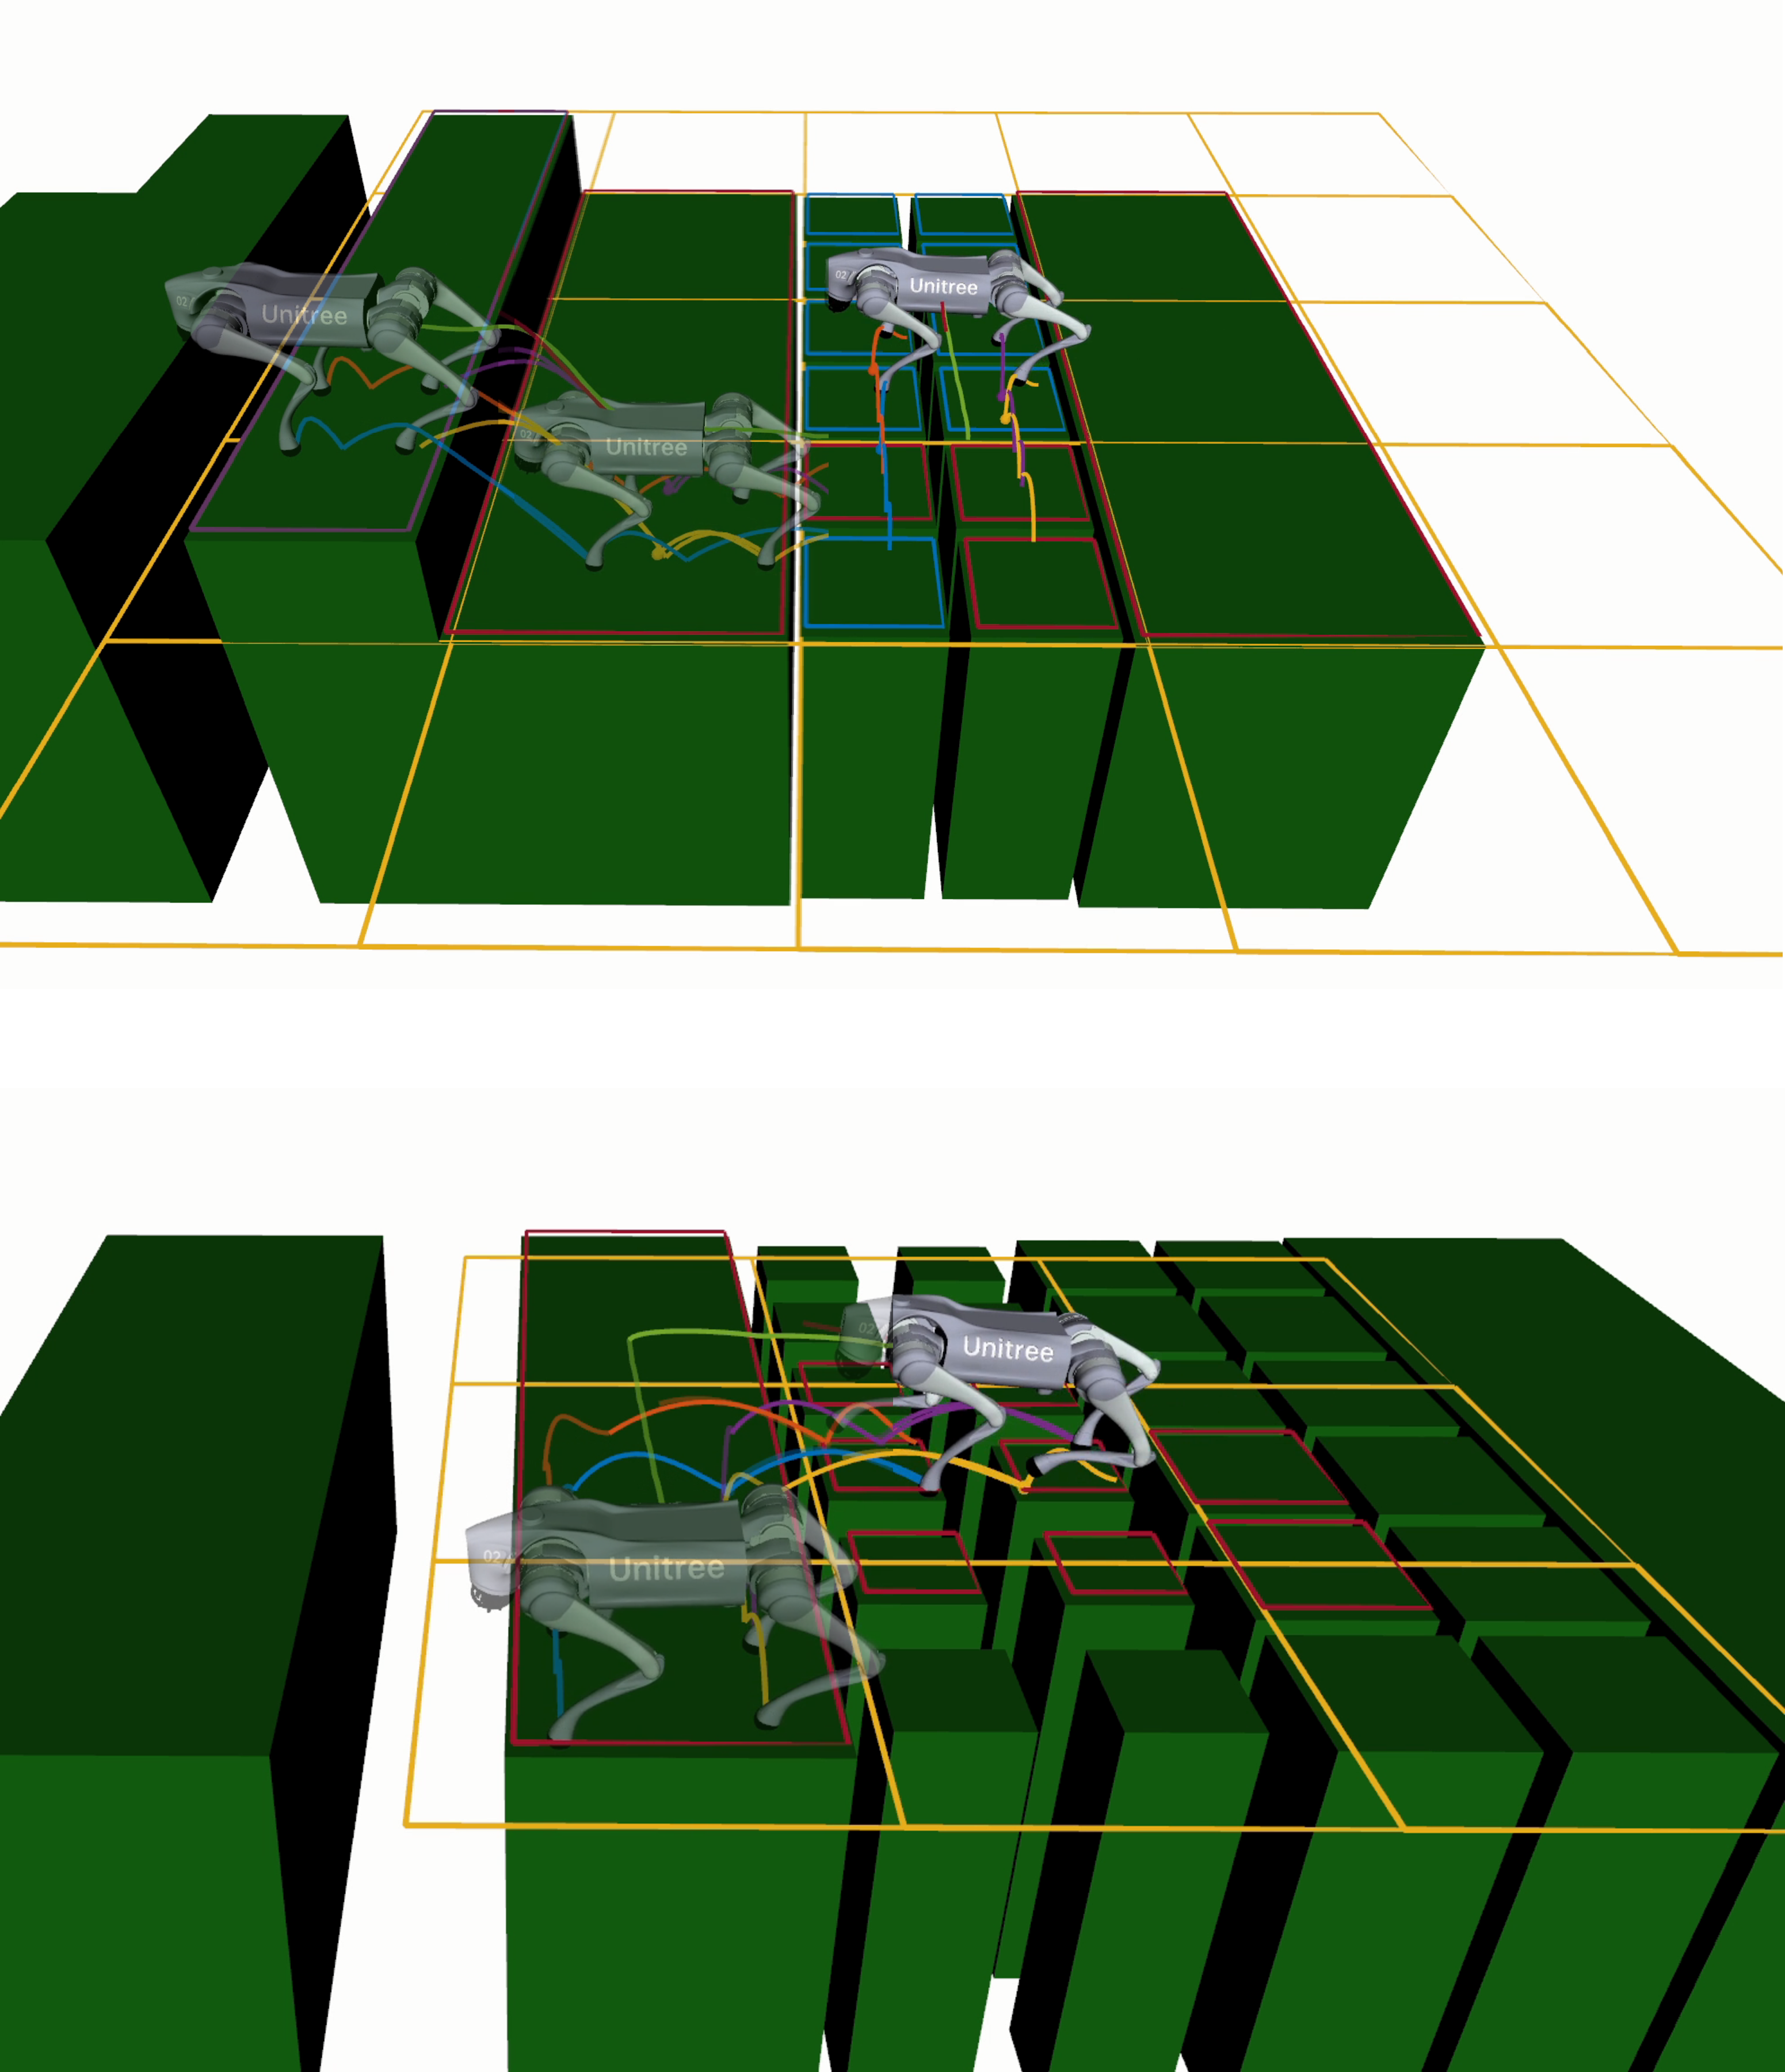
\includegraphics[width=\linewidth]{5x5_unstructured_demonstration.pdf}
%     \caption{Caption}
%     \label{fig:multiple_sizes}
% \end{figure}

\subsubsection{Unstructured Terrain}
% \begin{figure}
%     \centering
%     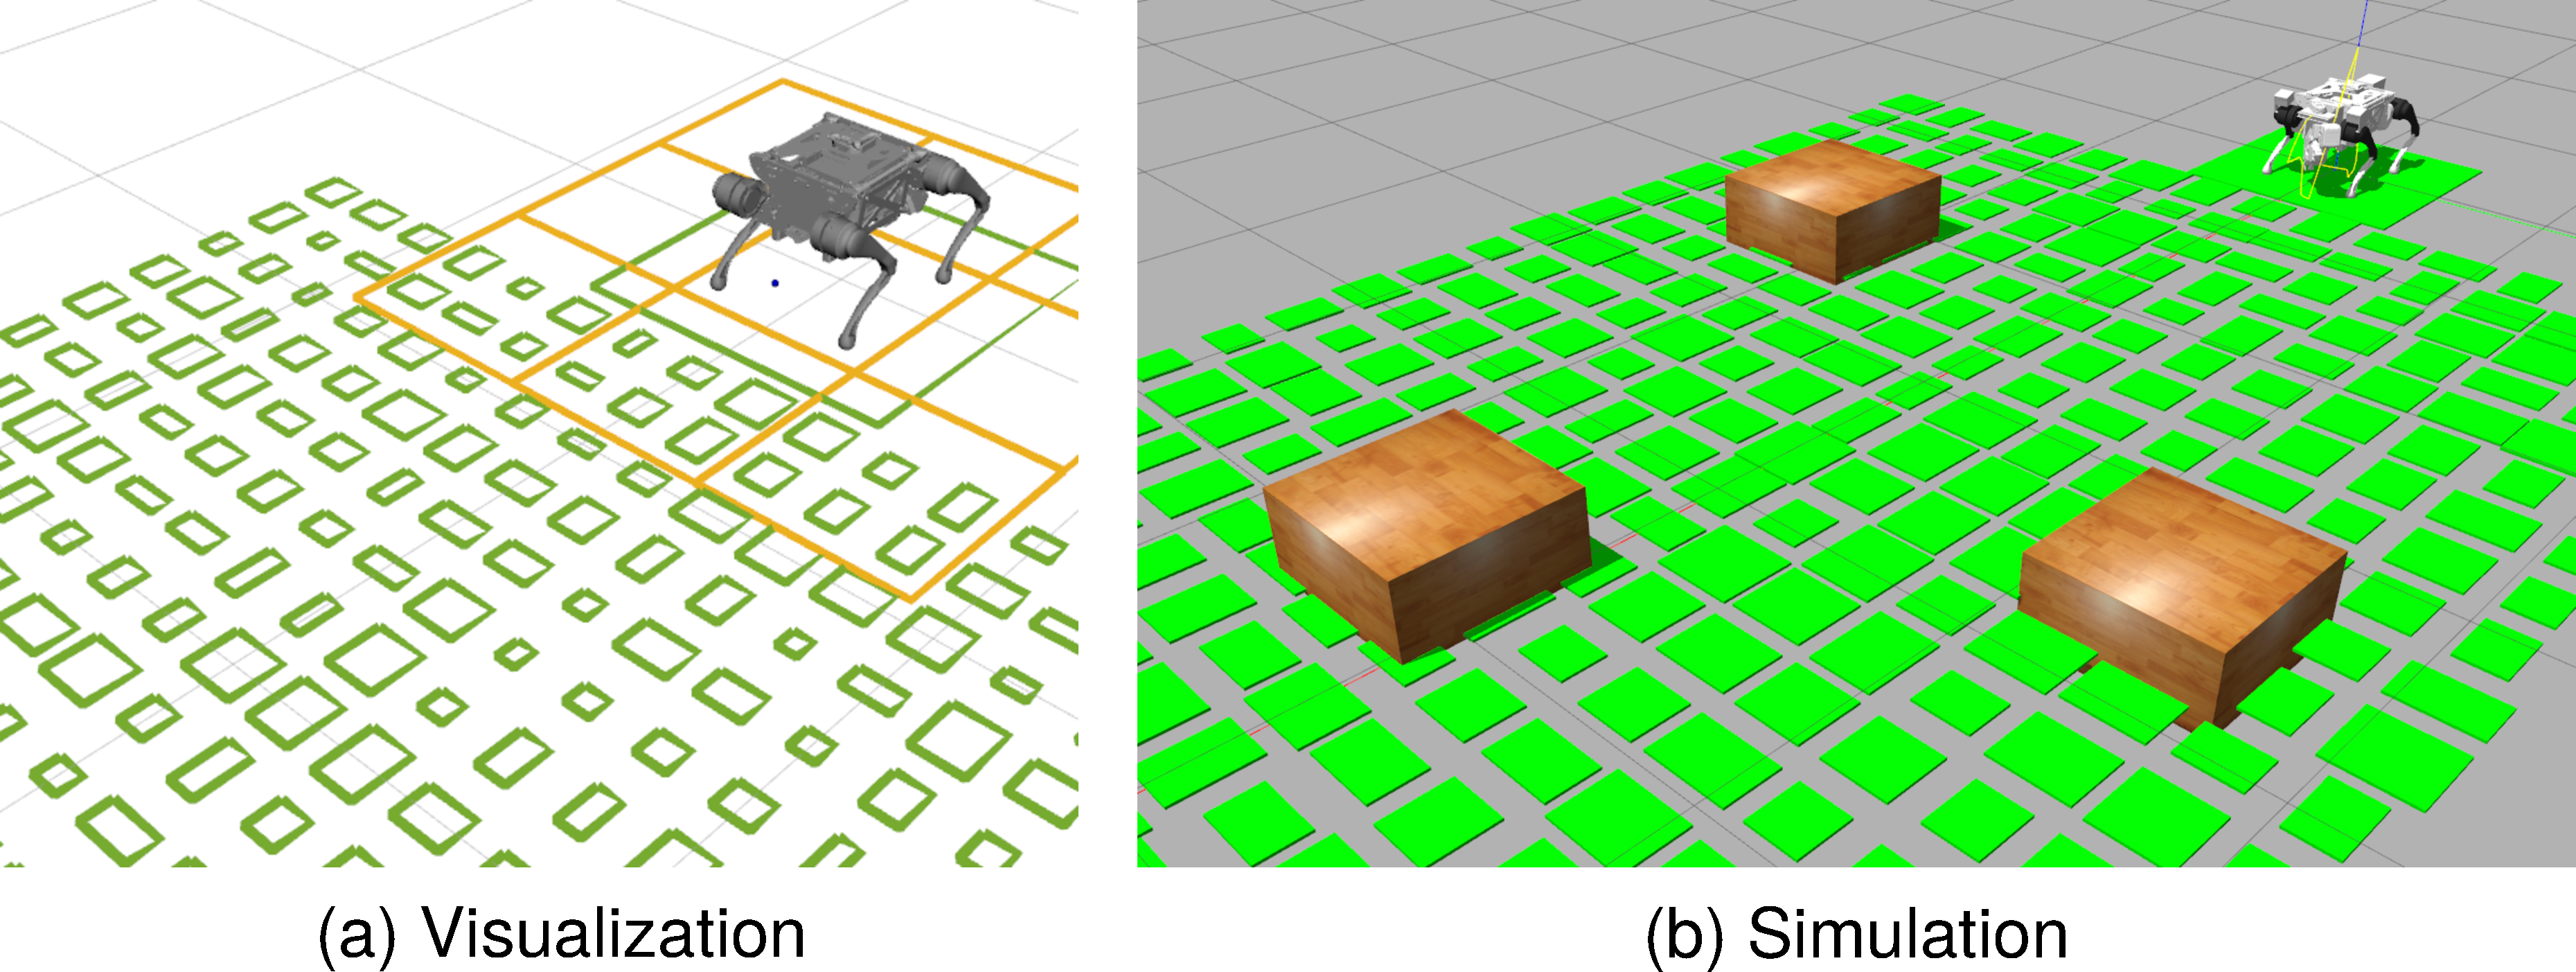
\includegraphics[width=\linewidth]{online_terrains.pdf}
%     \caption{(Will be updated to have rebar scenario.) Online scenarios with random sparsity of stepping stone and obstacles.}
%     \label{fig:online_terrains}
% \end{figure}
% Unlike Example \ref{example:1}, to further study the scalability of the proposed framework, 
We abstract 8 terrain types—\textit{flat terrain}, \textit{high terrain}, \textit{low terrain}, \textit{dense stone}, \textit{sparse stone}, \textit{gap}, \textit{high gap}, and \textit{low gap}—based on classification criteria involving polygon heights, counts, and areas relative to the abstracted grid cells. A terrain is categorized as a \textit{gap} when the ratio of its overlapping area with a grid cell falls below a specified threshold.
We define two terrain configurations: one consisting of four selected terrain types, and another comprising all eight. These are illustrated in Figs.~\ref{fig:online_terrains}(a) and \ref{fig:online_terrains}(b), respectively.
% \begin{figure}[h]
%     \centering
%     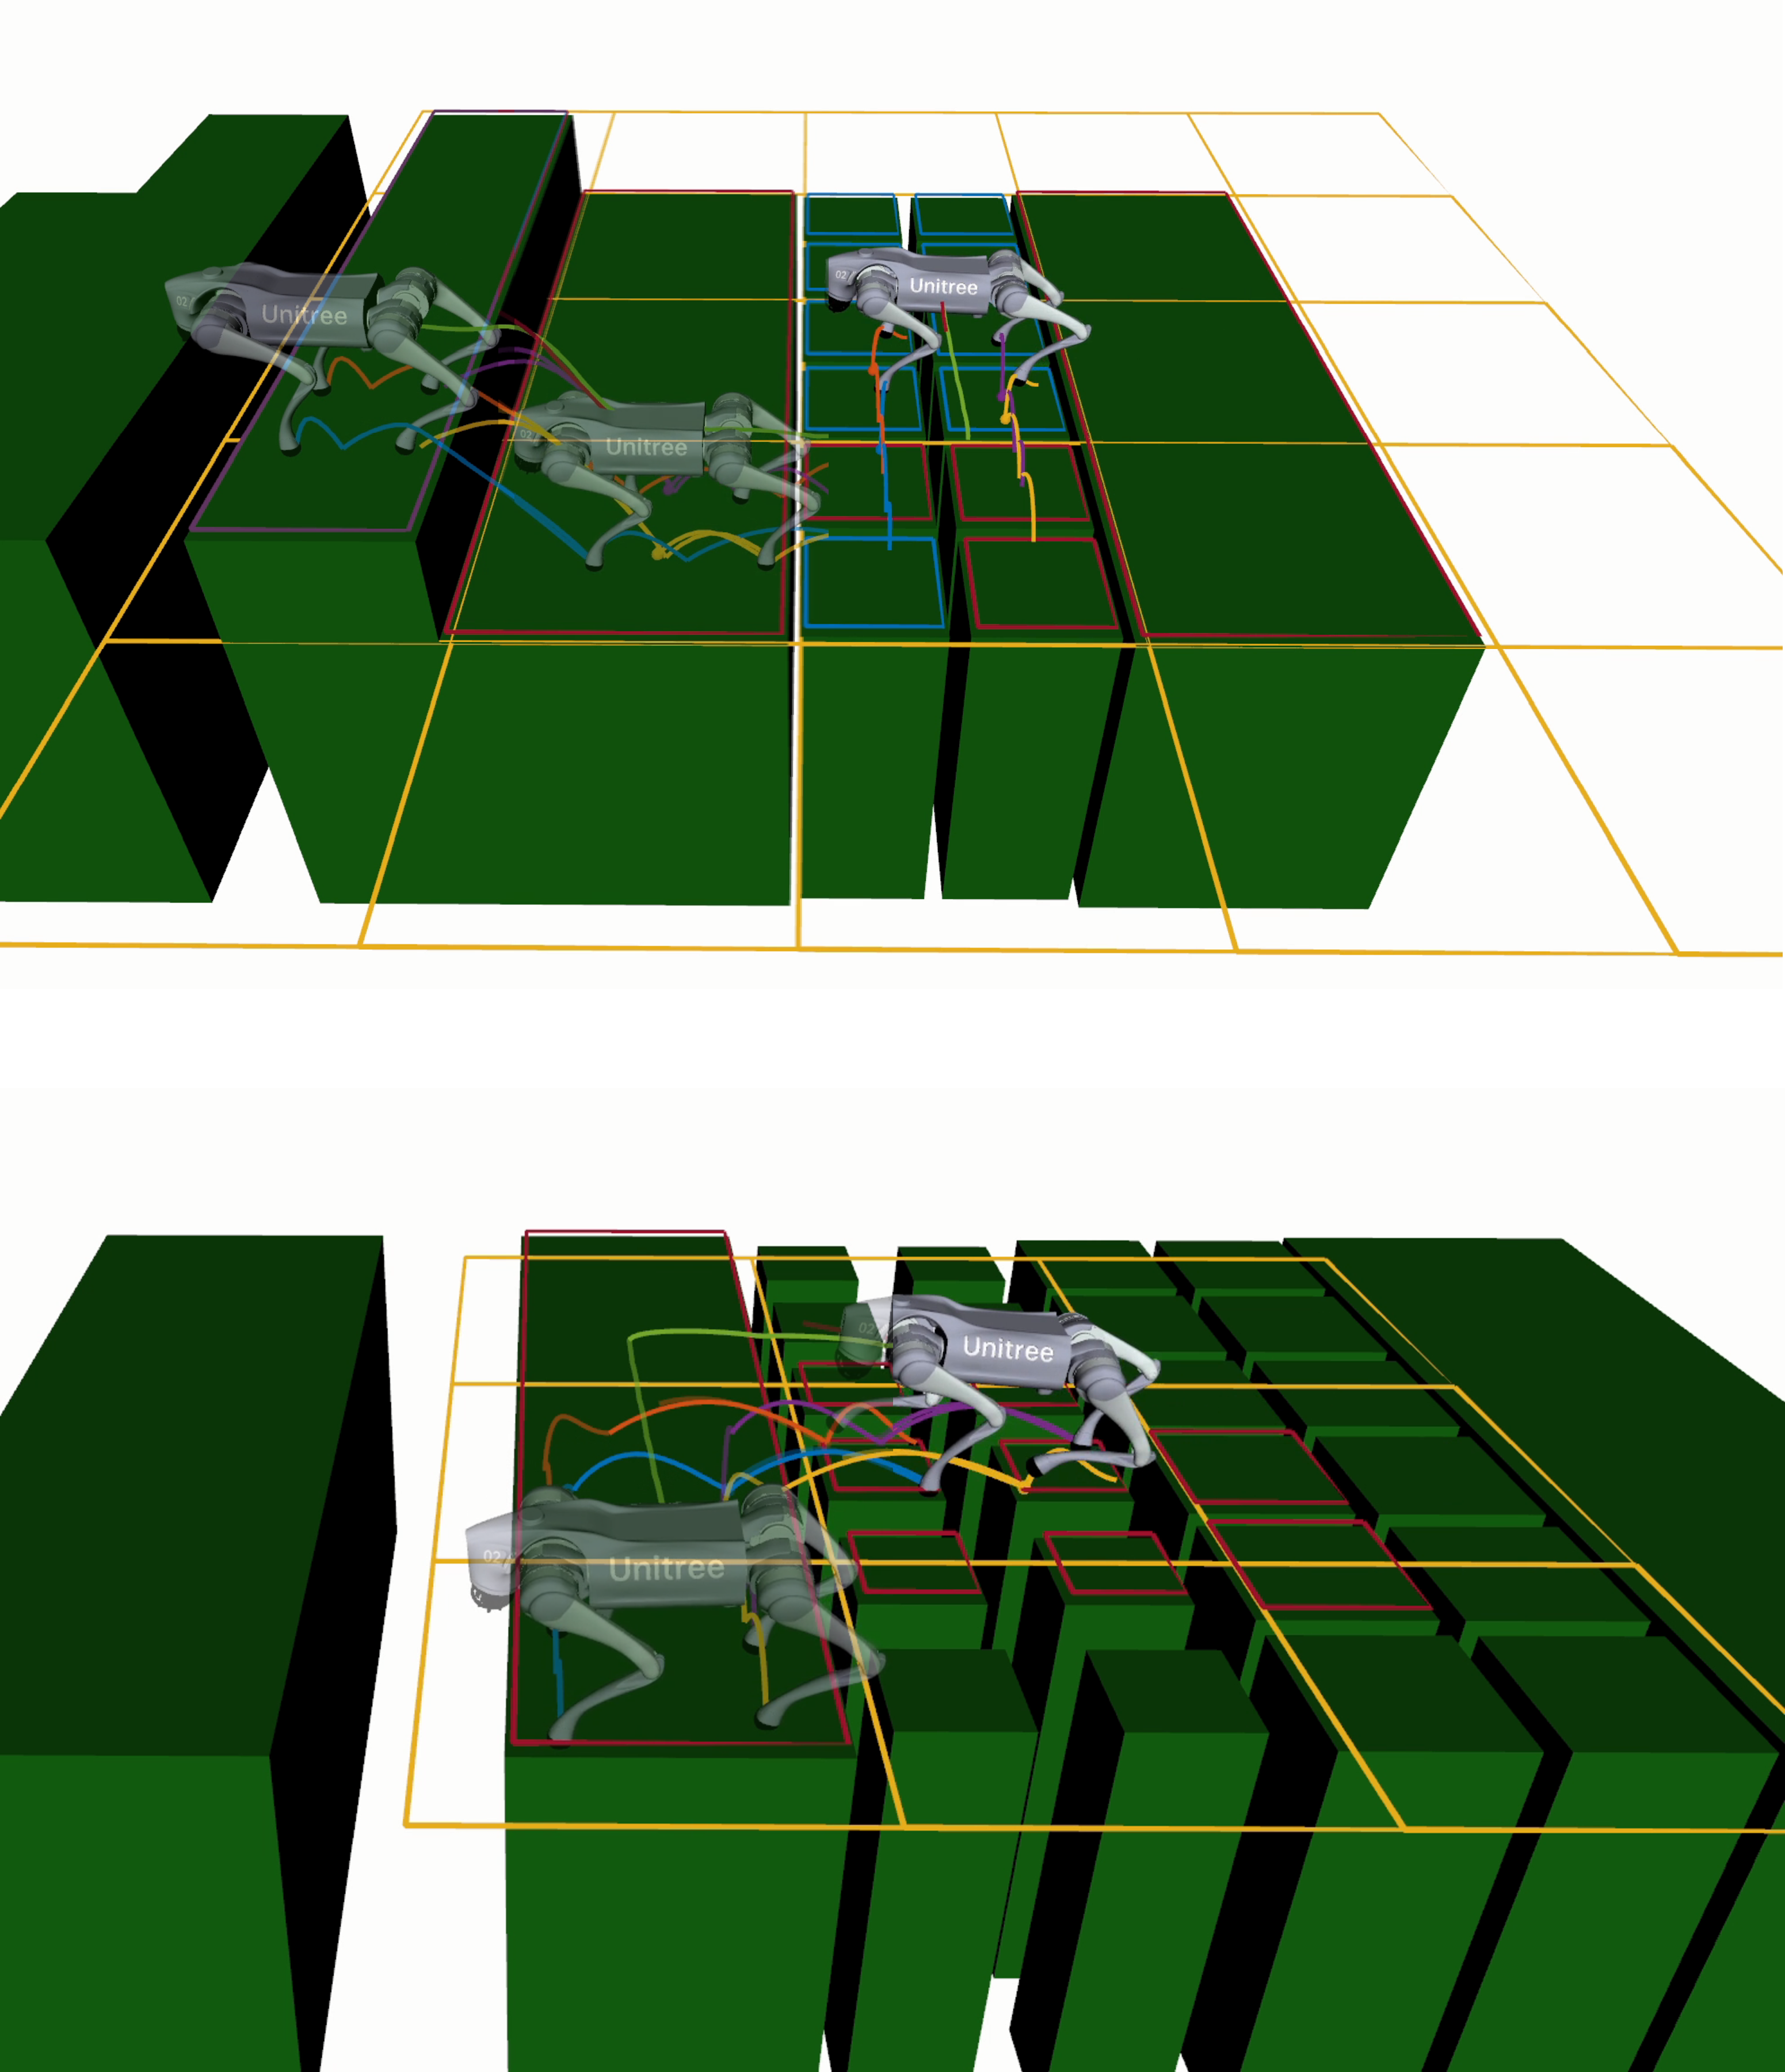
\includegraphics[width=\linewidth]{5x5_unstructured_demonstration.pdf}
%     \caption{Local environment abstraction and maneuvering with 5x5 (upper) and 3x3 (lower) grid size in separate unstructured terrain scenarios.}
%     \label{fig:multiple_sizes}
% \end{figure}

\subsubsection{Rebar Terrain}
% Inspired by automating labor-intensive rebar tying tasks on construction sites \citep{asselmeier2024hierarchical}, we explore a second case study where the quadrupedal robot navigates a rebar mat. 
% We model each rebar as a rectangular polygon with a 3 cm width. 
% Unlike the stepping stone scenario, this setup offers a larger number of potential stepping polygons due to the higher rebar density. 
% Observing that the robot's traversability depends on rebar sparsity in different directions—whether aligned with the robot's facing direction or not, 
% within a given tolerance—we abstract and classify rebar types based on a combination of horizontal sparsity (perpendicular to the robot's facing direction) and vertical sparsity (parallel to it). 
% %
% By calculating the number and relative spacing of the rebars inside each abstracted cell, we categorize each direction's sparsity as  \textit{dense} (0.05 - 0.15 m), \textit{sparse} (0.15 - 0.35 m), or \textit{extreme sparse} (above 0.35 m), \textit{single}, \textit{none}. 
% To reduce the complexity of the problem, we remove some challenging combinations such as \textit{none} or \textit{single} in both directions and treat them as \textit{obstacle}. As a result, we define two example configurations with 7 and 14 rebar terrain types. The 7-type scenario in Fig.~\ref{fig:online_terrains}(c) generates random rebar sparsity between 0.15 and 0.35 m, excluding the \textit{extreme sparse} type. In contrast, the 14-type scenario in Fig.~\ref{fig:online_terrains}(d)  includes rebar sparsity from 0.15 to 0.6 m, potentially covering more challenging combinations including the \textit{extreme sparse} ones.
Inspired by efforts to automate labor-intensive rebar tying tasks on construction sites \citep{asselmeier2024hierarchical}, we investigate a second case study in which a quadrupedal robot navigates a rebar mat. Each rebar is modeled as a rectangular polygon with a 3 cm width. Unlike the stepping stone scenario, this setup presents a denser distribution of potential footholds due to the higher rebar density. Notably, the robot’s traversability depends on the directional sparsity of the rebars—whether aligned with or orthogonal to the robot’s facing direction—within an acceptable tolerance.

We abstract and classify rebar types based on horizontal sparsity (perpendicular to the robot’s facing direction) and vertical sparsity (parallel to it). Within each abstracted cell, the number and spacing of rebars are evaluated to classify the sparsity in each direction as \textit{dense} (0.05–0.15 m), \textit{sparse} (0.15–0.35 m), \textit{extreme sparse} (above 0.35 m), \textit{single}, or \textit{none}. To reduce complexity, combinations deemed too challenging—such as \textit{none} or \textit{single} in both directions—are treated as \textit{obstacle}.
Based on this abstraction, we define two example configurations comprising 7 and 14 rebar terrain types. The 7-type configuration in Fig.~\ref{fig:online_terrains}(c) samples rebar sparsity randomly between 0.15 and 0.35 m, omitting \textit{extreme sparse} regions. In contrast, the 14-type configuration in Fig.~\ref{fig:online_terrains}(d) includes sparsity ranging from 0.15 to 0.6 m, encompassing more complex and difficult combinations including \textit{extreme sparse} types.
\begin{figure*}[t]
    \centering
    \includegraphics[width=\linewidth]{online_repair_new_gap.pdf}
    \caption{Runtime symbolic repair triggered by an unforeseen \textit{gap} state in the \textit{Unstructured-4} / $3\times 3$ scenario, in which gap states are deliberately excluded offline. Repair proposes the missing transition and gait-free MICP synthesizes a leaping skill, taking $12.36$\,s total ($0.18$\,s symbolic repair + $12.18$\,s gait-free MICP).}
    \label{fig:online_repair}
\end{figure*}

\begin{figure}[t]
    \centering
    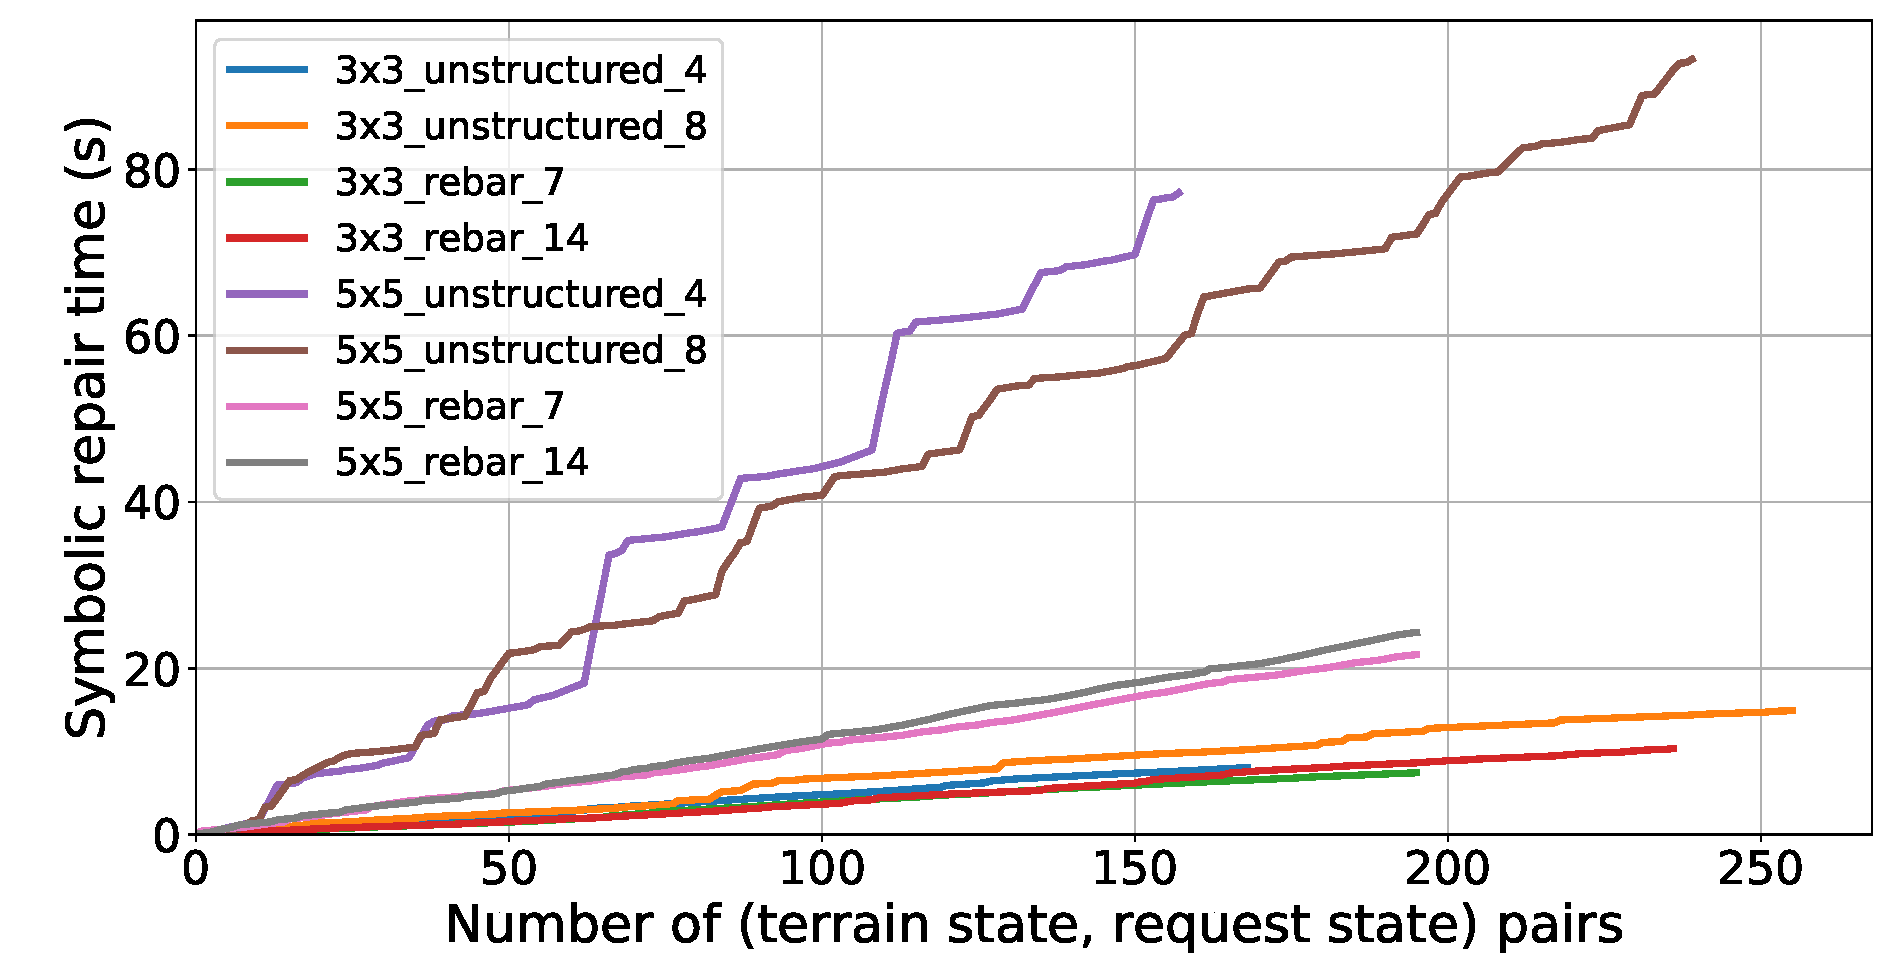
\includegraphics[width=\linewidth]{num_states_vs_repair_time.pdf}
    \caption{Offline symbolic-repair time versus the number of terrain--request state pairs for the $3\times 3$ and $5\times 5$ abstractions. Repair time grows approximately linearly in both cases; per state pair, the $5\times 5$ grid takes $478.1\%$ more time than the $3\times 3$ grid.}
    \label{fig:repair_vs_num_states}
\end{figure}

\begin{table*}
\centering
\small
    \caption{Online Gait-Fixed MICP Solving Time for Simulation}
    \setlength{\tabcolsep}{4pt}
     \begin{tabular*}{\linewidth}{@{\extracolsep{\fill}}cccccc}
         \hline
         \textbf{Scenario} & \textbf{Collision Avoidance} &
         \textbf{Binary Variables} &
         \textbf{Continuous Variables} &
         \textbf{Number of Polygons} &
         \textbf{Solve Time (s)}\\\hline
         Unstructured - 4 & No & 52 & 6583.5 & 6.5 & 0.37\\\hline
         Unstructured - 8 & Yes & \textcolor{red}{256} & 5166 & 2 & \textcolor{red}{2.65}\\
         & No & 69 & 7938 & 7.5 & 0.49\\\hline
         Rebar - 7& No & 70 & 7938 & 7.875 & 1.11\\
         \hline
         Rebar - 14 & No & 58 & 8142.75 & 6.25 & 1.09\\\hline
    \end{tabular*}
    \label{tab:micp_speed}
\end{table*}

\subsection{Offline Synthesis Results}
We evaluate the offline synthesis module for both \textit{Unstructured} and \textit{Rebar Terrain} scenarios by initializing the skill set with two trotting gaits ($2$ s and $3$ s). The inclusion of the longer-horizon trotting gait provides additional safer walking options from a practical standpoint. Prior to synthesis, we construct the set of possible terrain states $\inpstatesterrainexprposs$—assumed to be provided by the user—by systematically sweeping a local grid over the entire terrain map, based on the best available prior knowledge. The set of request states $\inpstatesrequestposs$ is defined as the top row of the local grid in the robot's facing direction, with the two corner cells also included to enable movement in diagonal directions.

% We briefly summarize the key offline synthesis statistics previously reported in \citep{zhou2025physically}. Specifically, the repair process was shown to successfully handle approximately $93.4\%$ of all terrain and request state pairs $(\inpstateterrain, \inpstaterequest) \in \inpstatesterrainexprposs \times \inpstatesrequestposs$. The remaining $6.6\%$ were unrepairable due to either unreachable request states caused by obstacles or physical infeasibility. Notably, the number of newly discovered skills was reduced by $71.6$–$97.6\%$ compared to checking the full space of all possible skills, each requiring the solution of a costly gait-free MICP. On average, generating a new locomotion gait via gait-free MICP took $27.23$ s, with a maximum time of $145.66$ s. These results demonstrate the effectiveness of the offline repair strategy in minimizing expensive MICP solves. For a full breakdown of synthesis time, number of symbolic states, and repair outcomes, please refer to \citep{zhou2025physically} (Table I).

Table~\ref{tab:offline_synthesis_time} reports 
\begin{enumerate*}[label=(\roman*),ref=\roman*]
    \item the number of terrain and request states pairs $(\inpstateterrain, \inpstaterequest) \in \inpstatesterrainexprposs \times \inpstatesrequestposs$, including both successful and total ones,
    \item the number of skills, 
    including the original,
    the newly discovered,
    and the total possible ones,
    and
    \item offline repair and feasibility checking times, including both from gait-fixed and gait-free MICP.
\end{enumerate*}
We first observe that the repair process successfully resolves $93.4\%$ of the terrain and request state pairs. The remaining cases are deemed unrepairable due to either unreachable request states caused by obstacles or inherent physical infeasibility. As highlighted in red, the number of newly discovered skills is reduced by $71.6$–$97.6\%$ compared to exhaustively checking all possible skills—each of which requires solving a computationally expensive gait-free MICP. On average, generating a new locomotion gait via gait-free MICP takes $27.23$ s, with a maximum of $145.66$ s. This demonstrates the effectiveness of offline repair in substantially reducing the number of costly gait-free MICP solves.


To investigate the scalability of offline repair,
we perform repair across various sizes of the terrain and request states.
As shown in
Fig.~\ref{fig:repair_vs_num_states},
the repair runtime grows linearly in the size of the terrain and request states for both $3\times 3$ and $5 \times 5$ grids.
While fewer terrain and request states handled offline reduce checked time, they may lead to more frequent unforeseen states during online execution.
%
Moreover, we note that
the slope of $5 \times 5$ cases in Fig.~\ref{fig:repair_vs_num_states}
are steeper than those of $3\times 3$
% because 
as a result of the increased state space.
% We further note that 
On average,
repair takes 478.1$\%$ more time for $5\times 5$ grids than $3\times 3$ for one terrain and request states pair.
% However, 
%
In practice, 
the perception range and the robot size limit the grid size, 
so we do not test beyond $5\times 5$ grids,
though the user can adjust the resolution.

\begin{figure*}[t]
    \centering
    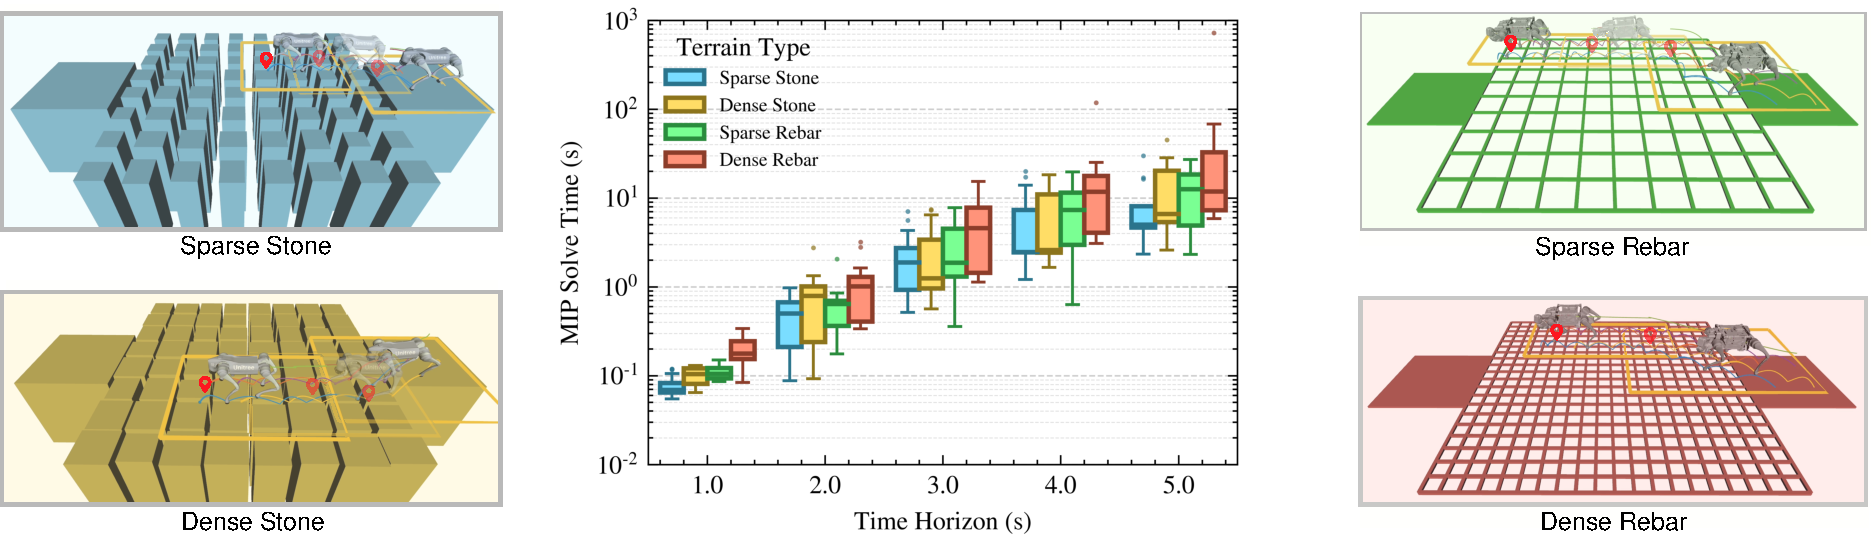
\includegraphics[width=\linewidth]{pure_mip_benchmark_box_plot.pdf}
    \caption{\revised{MIP solve time across four terrains---sparse stone (blue), dense stone (yellow), sparse rebar (green), dense rebar (red)---and horizons of $1$--$5$\,s, as box plots over $10$ seeded waypoints per scenario. In each terrain subfigure, selected traversal snapshots at planning horizons of $1$\,s (blue), $2$\,s (yellow), $4$\,s (green), and $5$\,s (red) are overlaid for visualization.}}
    \label{fig:pure_mip_benchmark}
\end{figure*}

\begin{figure}
    \centering
    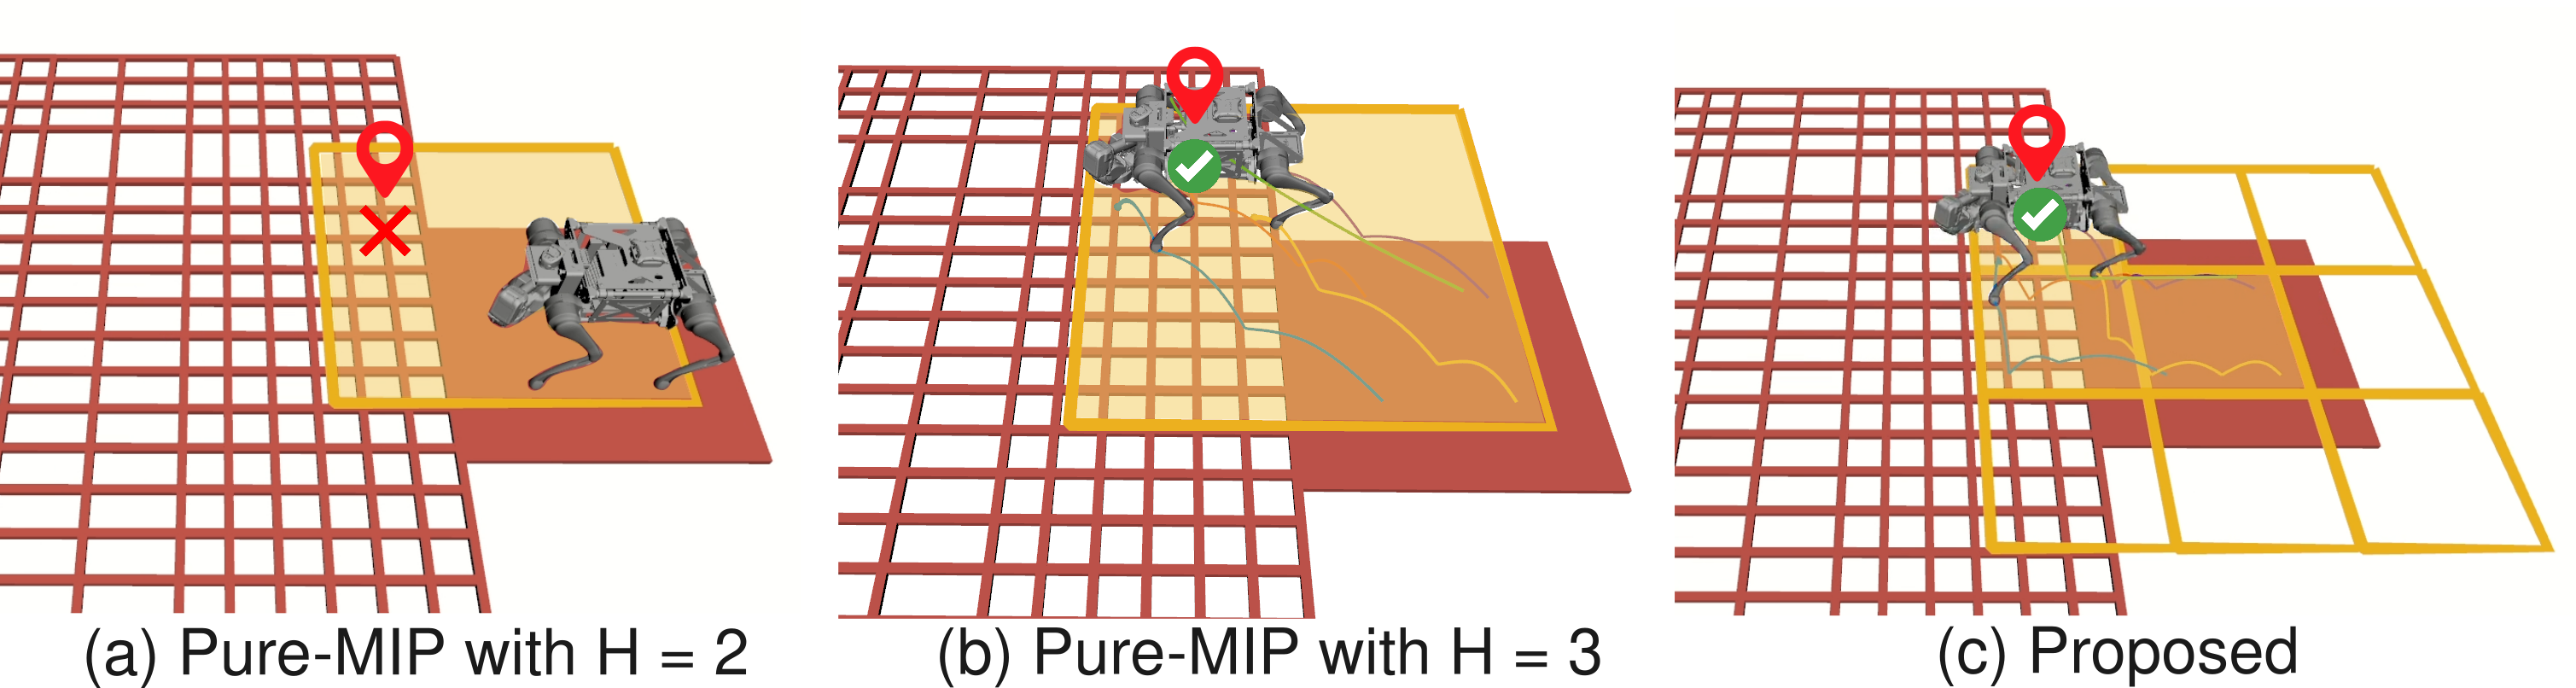
\includegraphics[width=\linewidth]{dense_rebar_comparison.png}
    \caption{\revised{Representative dense rebar trial after randomly removing terrains for benchmarking different baselines: (a) Pure-MIP with $H{=}2$ s; (b) Pure-MIP with $H{=}3$ s; (c) Proposed approach with $3\times 3$ grid.}}
    \label{fig:dense_rebar_comparison}
\end{figure}

\subsection{Online Execution Results}
Fig.~\ref{fig:online_terrains} presents snapshots of Go2 and Chotu navigating various terrains during online execution. The robot is tasked with reaching a global waypoint using a naive global shortest-path planner. At each step, the local waypoint is selected as the closest non-obstacle cell in the local grid map pointing toward the global target.

In Fig.~\ref{fig:online_terrains}(a), the robot traverses a sequence of terrain types including \textit{flat terrain}, \textit{dense stepping stone}, \textit{sparse stepping stone}, and \textit{gap}. Fig.~\ref{fig:online_terrains}(b) showcases a more complex maneuver involving all eight terrain types, including elevation changes, where the robot adaptively selects suitable locomotion gaits. Similarly, Figs.~\ref{fig:online_terrains}(c) and (d) illustrate Chotu traversing rebar terrains with 7 and 14 defined rebar types, respectively.
Notably, the robot utilizes newly discovered leaping gaits with short aerial phases to execute challenging transitions—such as moving from lower to higher elevations or crossing over gaps and \textit{extreme sparse} rebar segments, as demonstrated in Figs.~\ref{fig:online_terrains}(b) and(d).

Table \ref{tab:micp_speed} summarizes the average number of decision variables, terrain polygons, and solve time for each scenario, computed across all step transitions in a full locomotion run with the online gait-fixed MICP.
%\ye{[why the number of continuous variables has decimal digits?]}\ziyi{[The planner could choose adaptive gaits with different time horizons.]} \ye{[Ok, then we should provide some more info on how the average number is calculated. Is it based on 100 trials randomly selected or under certain trial conditions?]} \ziyi{[Rephrased this sentence. It's averaged only because each maneuver includes multiple transitions and solve MICP multiple times.]} \ye{[can we say "across all step transitions during one full locomotion run?"]\ziyi{Done}}
On average, the online gait-fixed MICP takes $430$ ms to solve the unstructured terrain cases and $1.1$ s for rebar cases when the collision avoidance is disabled. 
% the time horizon ranges from $1.5$ s to $3.0$ s, 
% depending on the chosen gait. 
The rebar scenarios exhibit $155.8\%$ longer solve times due to their overlapping, skewed rebar arrangement, and a larger number of terrain polygons. 
Additionally, 
enabling 
collision avoidance (necessary for \textit{Unstructured - 8} case to handle the elevation change) 
increases the number of binary variables
by $271.0\%$, 
increasing the solve time 
% to $2.65$ s.
by $440.8\%$
(highlighted in red).

\revised{\subsection{Runtime Repair Case Study}\label{sec:runtime_repair_case_study}
As a case study to demonstrate the framework's capability to handle unforeseen terrains and online failures, we highlight the following run-time scenarios that trigger runtime repair or re-synthesis.

\subsubsection{Unforeseen Terrain States}
With limited prior knowledge of the global terrain map, the terrain states provided during offline synthesis may be insufficient when encountering new terrain configurations. Fig.~\ref{fig:online_repair} illustrates this in an \textit{Unstructured - 4 types} scenario with a $3 \times 3$ grid size, where terrain states involving \textit{gap} terrain are deliberately excluded from the offline phase. When the robot reaches a new terrain state that contains a \textit{gap}, runtime repair is triggered for the current terrain and request states. A new skill with a leaping gait is generated to successfully cross the gap. The runtime repair takes $12.36$\,s in total, of which the symbolic-repair stage accounts for $0.18$\,s and the gait-free MICP for the new leaping gait accounts for $12.18$\,s---confirming that the dominant cost lies in the dynamic-feasibility check, not the symbolic search.

\subsubsection{Solving Failure}
Another common runtime failure arises from MICP solving failures. Due to discrepancies between the predefined polygons used during offline synthesis and the actual online terrains---such as variations in shape and size---a skill deemed feasible offline may become infeasible when executed online, even if classified under the same symbolic transition. The detours shown in Fig.~\ref{fig:online_terrains}(c) and (d) illustrate the re-synthesis process triggered by solving failures in the 7-type and 14-type rebar cases. Solving failures occur more frequently in the rebar scenarios than in the unstructured ones, due to the higher uncertainty in the shapes and sizes of online rebar polygons. Re-synthesis takes $0.11$\,s and $0.07$\,s respectively for the two cases. Neither case triggers full runtime repair, because the existing skill set suffices to navigate to the goal under the failed transition.}

\subsection{Benchmark: Pure-MIP Planner}
To evaluate how the symbolic-continuous planner separation benefits the overall planning framework, we benchmark our method against \textit{pure-MIP} approaches, where we implement a planner to evaluate how computation time scales with the planning horizon and terrain complexity. \revised{The pure-MIP approach can also be treated as an ablation study for the symbolic planning.} Specifically, we examine five planning horizons ranging from $1$ s to $5$ s. In addition, we vary the terrain types by considering sparse stepping stones (0.15 m spacing), dense stepping stones (0.05 m spacing), sparse rebar (0.3 m spacing), and dense rebar (0.15 m spacing), as illustrated in Fig.~\ref{fig:pure_mip_benchmark} with specific colors.

\revised{To make the comparison precise: the pure-MIP baseline uses the \emph{same} convex relaxations of the dynamics (Eq.~(\ref{eq:dynamics})), the \emph{same} linearized friction-cone and fixed-Jacobian kinematic constraints, and the \emph{same} cost weights as our online gait-fixed MICP. The only differences are (i) the planner solves a single long-horizon gait-fixed MICP without symbolic-level decomposition, and (ii) the local planning region is expanded to encompass all terrain polygons within the horizon-induced reachable distance, rather than being limited to the cells adjacent to a symbolic transition. The same Gurobi solver and settings are used in both cases.}

\revised{The pure-MIP planner uses an \emph{adaptive} local region whose maximum size scales with the planning horizon $H$ (in seconds): along each axis the region spans up to $\textrm{gs} + (\textrm{gs}/2)\cdot H$, where $\textrm{gs}$ is the symbolic-cell grid spacing, with a floor of $1.5\,\textrm{gs}$ corresponding to the $H{=}1$\,s setting. So the $H{=}2$\,s column reads as a like-for-like comparison for an equivalent two-cell transition footprint, while each additional second of horizon adds half a cell of reach. As shown in Fig.~\ref{fig:pure_mip_benchmark}, the region further shrinks when the goal lies within the maximum range, avoiding redundant incorporation of terrain polygons in each MIP solve. 
% so the per-MIP foothold set always stays proportional to the distance the gait can traverse in one solve. 
In contrast, our proposed planner always plans against a fixed $3{\times}3$ symbolic grid centered on the robot, decoupling the per-MIP problem size from the total traversal distance. We omit the gait-free MICP from the benchmark because its solve time becomes prohibitively long once $H>2$\,s; the locomotion gait is repeated cyclically on a $1$\,s trotting pattern, and the planner receives a global waypoint and incrementally computes local waypoints as in the proposed framework.}

\revised{Fig.~\ref{fig:pure_mip_benchmark} also reports the per-MIP solve time as box plots aggregated over $10$ randomly sampled waypoints per scenario. Within the same terrain, the solve time grows almost exponentially with the horizon, and the dense variants consistently take longer than their sparse counterparts because more terrain polygons enter the MIP. The $H{=}1$\,s setting is too myopic to commit to scenarios that require multi-step planning, while $H\ge4$\,s pushes the median solve into multiple seconds even for the easier scenarios. The $H{=}2$\,s and $H{=}3$\,s horizons sit on the knee of this trade-off curve, balancing optimality and per-step compute, and we therefore adopt them as the two reference pure-MIP configurations for the end-to-end benchmark below.}

\revised{To assess closed-loop behavior beyond a per-MIP solve time, we run an end-to-end comparison on the dense rebar scenario, where the pure-MIP planner is most stressed. For each method, we dispatch $10$ seeded random waypoints; between trials the robot is reset back to the launch pose, and we randomly remove a fraction of the rebar polygons as shown in Fig.~\ref{fig:dense_rebar_comparison} to add randomness and make the scenario more challenging. Identical random seeds across methods ensure all baselines see the byte-for-byte same waypoints and terrain, so any difference in outcome reflects the planner alone. Fig.~\ref{fig:dense_rebar_comparison} also shows one representative instance on which the pure-MIP planner with short horizons (i.e., 1 or 2 s) stalls---the planning region is too limited for the solver to discover a feasible routing path% the resulting foothold pattern forces the MIP to at most backtrack within its local region and the planner has no mechanism to deliberate at the symbolic level about which neighboring cell to attempt next
, whereas the proposed planner routes through a sequence of cells.}

\revised{Table~\ref{tab:pure_mip_benchmark} reports the success rate, mean traversal time of successful trials, and the mean per-module active computation per trial---broken down into MIP transition solving, the pre-flight MIP feasibility check (FC), reactive synthesis (strategy query plus strategy reload), and runtime repair (online specification regeneration). In this scenario, the proposed planner attains $90\%$ success rate with $18.5$\,s mean traversal time, matching the $H{=}3$\,s pure-MIP success rate ($90\%$) at roughly three quarters of the traversal time and at less than half the MIP transition cost ($5.26$\,s vs.\ $11.54$\,s per trial). The shorter $H{=}2$\,s pure-MIP setting reaches only $60\%$, indicating that its horizon is too myopic to recover from the gaps. The two ablation rows confirm the value of the online additions introduced in this work: disabling the FC drops the success rate substantially in both planners ($60\%\rightarrow20\%$ for pure-MIP at $H{=}2$\,s and $90\%\rightarrow60\%$ for the proposed planner); disabling the delay-aware coordination (DAC) preserves the $90\%$ success rate of the proposed planner but inflates the mean traversal time from $18.5$\,s to $23.4$\,s, because each symbolic transition now must wait for the previous trajectory to be fully tracked before the next MIP solve can start.}

\begin{table*}[t]
\centering
\caption{\revised{End-to-end benchmark on the dense rebar scenario ($10$ seeded waypoints, identical seed and terrain across methods, with randomly removed rebars per trial to add randomness). Traversal time and per-module times are mean values computed over successful trials only. Reactive synthesis combines the per-step strategy query and the per-spec-switch strategy reload. Dashes denote modules that do not exist in the corresponding method or are disabled by the ablation.}}
\label{tab:pure_mip_benchmark}
\setlength{\tabcolsep}{4pt}
{\color{blue}
\begin{tabular}{lcccccc}
\hline
\textbf{Method} & \textbf{Success} & \textbf{Traversal} & \textbf{MIP trans.} & \textbf{MIP feas.} & \textbf{Reactive synth.} & \textbf{Runtime repair} \\
 & \textbf{rate} & \textbf{time (s)} & \textbf{solving (s)} & \textbf{check (s)} & \textbf{(query + load, s)} & \textbf{(s)} \\
\hline
Pure MIP ($H{=}2$\,s)                              & 60\% (6/10) & 14.76 &  3.04 & 0.21 & --   & --   \\
Pure MIP ($H{=}3$\,s)                              & 90\% (9/10) & 24.73 & 11.54 & 0.19 & --   & --   \\
Pure MIP ($H{=}2$\,s), no FC        & 20\% (2/10) &  9.00 &  1.38 & --   & --   & --   \\
Pure MIP ($H{=}3$\,s), no FC        & 40\% (4/10) & 14.23 &  5.17 & --   & --   & --   \\
\hline
Proposed                                           & 90\% (9/10) & 18.48 &  5.26 & 0.19 & 0.29 & 0.03 \\
Proposed, no FC                     & 60\% (6/10) & 20.08 &  5.85 & --   & 0.33 & 0.05 \\
Proposed, no DAC & 90\% (9/10) & 23.43 &  5.11 & 0.27 & 0.28 & 0.04 \\
\hline
\end{tabular}
}
\end{table*}

\subsection{Preliminary Study: Yaw Command Extension}\label{sec:extension}
\begin{figure}
    \centering
    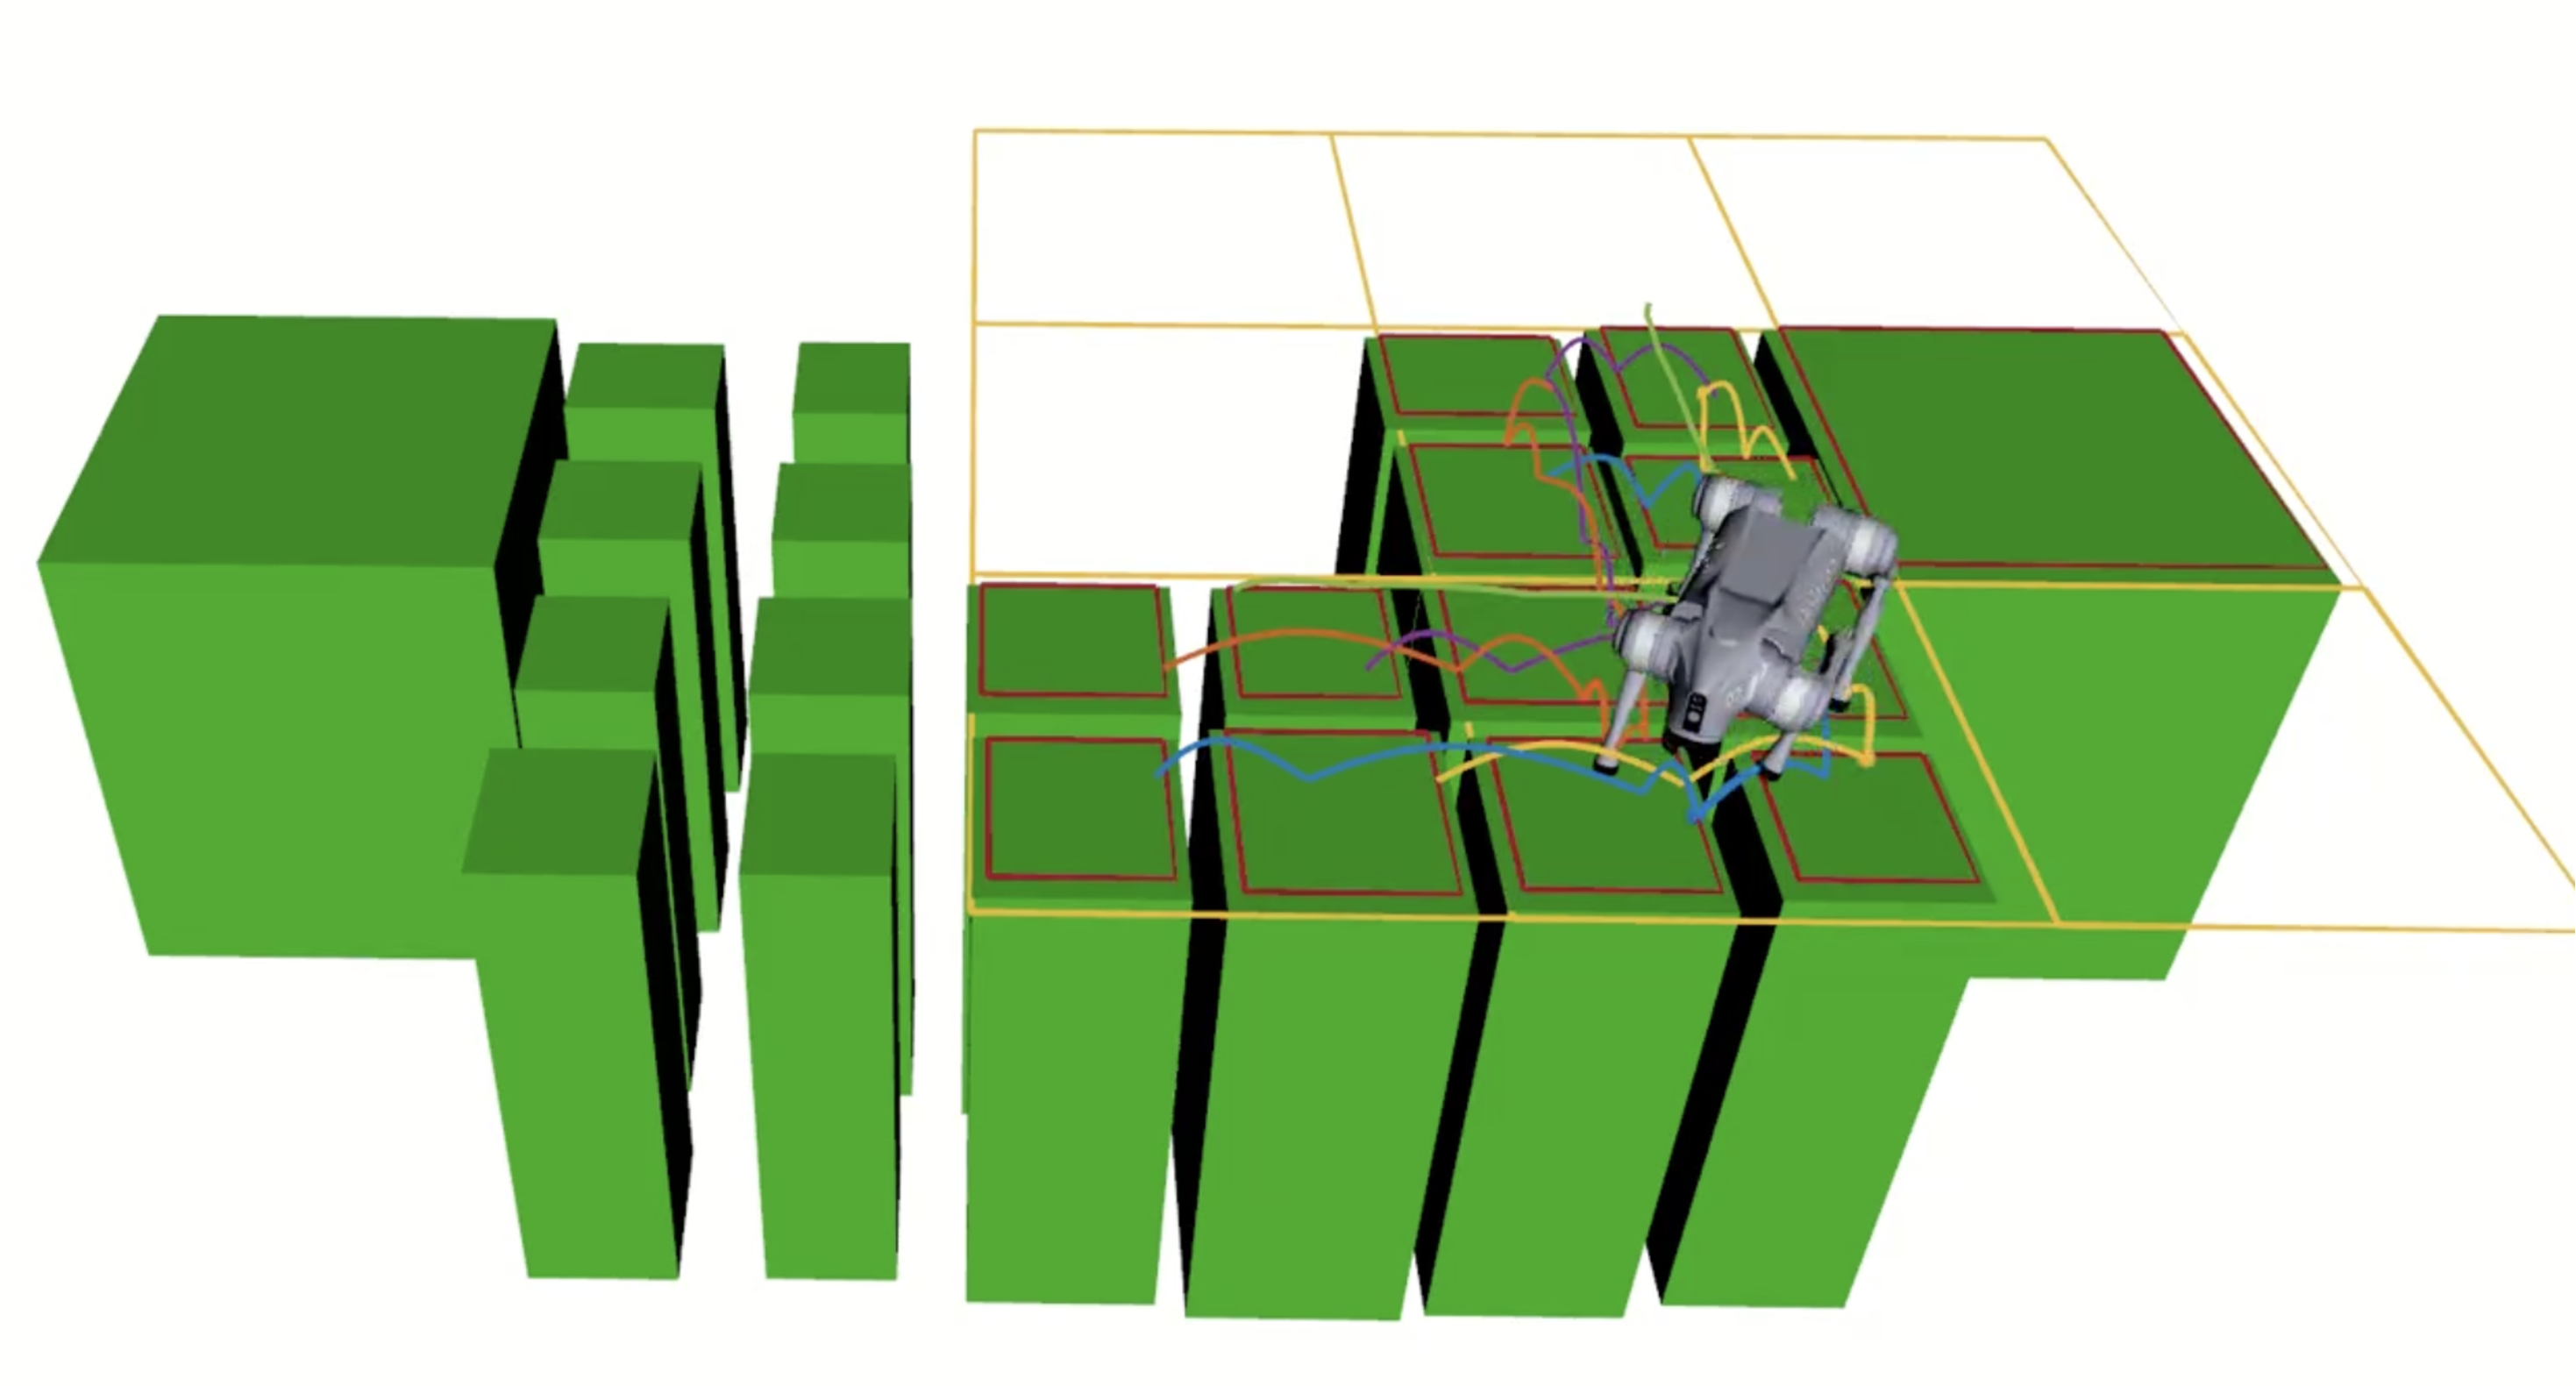
\includegraphics[width=\linewidth]{yaw_extension_demo.pdf}
    \caption{Demonstration of the robot executing multiple turning behaviors to continuously progress toward the global waypoint on terrain arranged in a zig-zag pattern.}
    \label{fig:yaw_extension}
\end{figure}
\revised{This subsection demonstrates that the proposed framework can be extended to non-zero yaw waypoints in principle, but we report the result as a \emph{preliminary feasibility study} only. We do not claim a full demonstration of generalizability of any angular movements. Specifically: (i) the symbolic abstraction in Sec.~\ref{sec:preliminaries_abstraction} grows combinatorially when yaw is added as a discretized input, and we have not characterized how the manager and symbolic-repair scaling numbers reported in Sec.~\ref{sec:experiments} change with yaw discretization; (ii) the angular-momentum coupling neglected by the convex-dynamics simplification in Eq.~(\ref{eq:dynamics}) becomes more relevant once yaw is treated as a planned variable, especially for fast turns; (iii) we report simulation results only---no hardware deployment of the yaw extension.}

In the previous examples, we assume that the yaw angle of the robot base is fixed to simplify the problem. However, the robot's physical capability to traverse terrains largely depends on the base orientation. For instance, performing a forward jump onto a high terrain is different from a sideway jump, in terms of both leg kinematics and dynamics.
Therefore, to demonstrate the framework's modularity, we provide a preliminary extension to the existing abstraction of the robot state to allow yaw variation.

Specifically, the robot inputs are now defined as
$\inpcen \coloneqq 
\{\var_x \mid x \in \xcells\} \cup 
\{\var_y \mid y \in \ycells\} \cup \{\var_{yaw} \mid yaw \in \mathcal{W}\}$, where we define a new set of yaw angles $\mathcal{W} \coloneqq \{-180 \degree, -90 \degree, 0 \degree, 90 \degree, 180 \degree\}$. Note that, a finer discretization of the yaw angles can be defined as needed.
Similarly, the request inputs are defined as 
$\inprequest \coloneqq
\{\var_x^\textrm{req} \mid x \in \xcells\} \cup 
\{\var_y^\textrm{req} \mid y \in \ycells\} \cup \{\var_{yaw}^\textrm{req} \mid yaw \in \mathcal{W}\}$. The robot and the request input can be further divided into translational 
$\inpcentrans, \inprequesttrans$ and rotational parts $\inpcenorien, \inprequestorien$, where the translational ones contain the $x$ and $y$ states and the orientational ones contain the $yaw$ state.

The skill is further divided into translational and rotational skills. A translational skill $\skill_{\textrm{trans}} \in \out_{\textrm{trans}}$
consists of 
sets of preconditions $\skillpretrans \subseteq \inpstatescen \times \inpstatesterrain$ that include the full robot state, and 
% a set of 
translational-only postconditions $\skillposttrans \subseteq \inpstatescen^{\textrm{trans}}$. A rotational skill in place $\skill_{\textrm{orien}} \in \out_{\textrm{orien}}$ consists of sets of rotational-only preconditions $\skillpreorien \subseteq \inpstatescen^{\textrm{orien}}$ and postconditions $\skillpostorien \subseteq \inpstatescen^{\textrm{orien}}$. The terrain state can also be incorporated when generating rotational skills, particularly for terrains that pose challenges for turning. However, we omit this in our current implementation for simplicity. The specification encoding then follows the same procedure as described in Sec.~\ref{sec:spec_gen}, based on each skill's precondition and postcondition. The hard constraints remain unchanged, except that translational and rotational ones are defined separately to ensure the corresponding states remain unchanged when no skill is selected.

To demonstrate the resulting maneuver, we construct a scenario with multiple dense and sparse stepping stones arranged in an overall zig-zag pattern, requiring several turning behaviors. Although sideways movement skills are feasible, we manually exclude them before synthesis to highlight yaw adjustments controlled by the rotational skills. As shown in Fig.~\ref{fig:yaw_extension}, the robot executes multiple turns to continuously progress towards the global waypoint. More complex coupled translational and rotational behaviors can also be defined by modifying the preconditions and postconditions associated with each skill.

% \subsubsection{Diagonal Movement}\label{sec:extension_diag}




\section{Hardware Demonstrations}\label{sec:hardware}
\begin{figure*}[t]
    \centering
    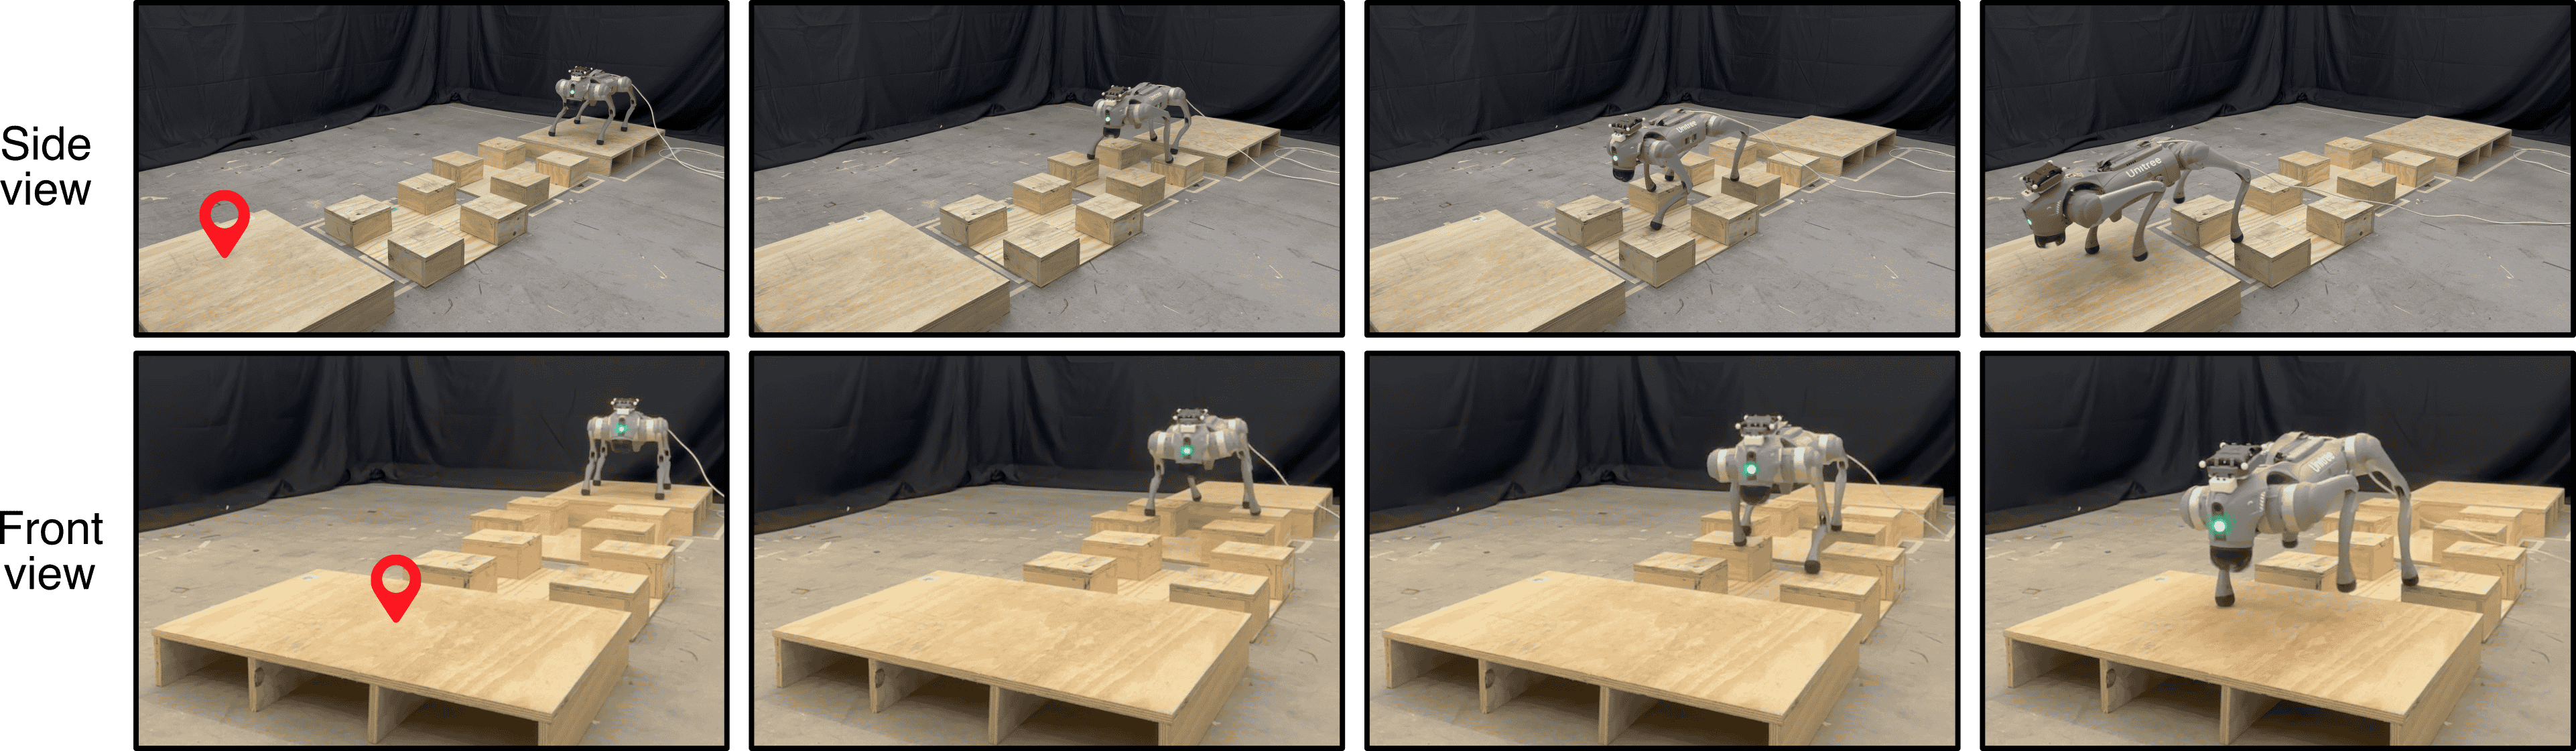
\includegraphics[width=\linewidth]{unstructured_hardware_withoutgap_compressed.png}
    \caption{Hardware experiment on the first unstructured-terrain scenario: sparse stepping stones ($0.18$--$0.23$\,m apart) interleaved with flat regions. Side and front views highlight the lateral misalignment of the stones; the online MICP produces a sideways trajectory and a $3$\,s trotting gait is used throughout.}
    \label{fig:hardware_withoutgap}
\end{figure*}
We demonstrate that our entire framework can be successfully deployed on hardware, highlighting two key aspects. First, we showcase the framework’s capability to generate adaptive locomotion gaits across diverse terrain types, particularly focusing on agile leaping motions. Second, we illustrate the framework’s assured safety through obstacle avoidance and selection of dynamically feasible gaits, benchmarked against a heuristic-based planner.
\subsection{Hardware Experiment Setup}
For hardware experiments, we set up similar real-world scenarios for both unstructured and rebar terrains. For the unstructured terrain scenario, we construct wooden blocks to form stepping stones, gaps, and flat regions, with each stepping stone elevated approximately $0.12$ m above the ground. For the rebar scenario, we assemble a realistic rebar mat using fourteen $1/2$-inch $\times$ $4$-foot rebars and six $1/2$-inch × $10$-foot rebars.
In the synthesis setup, obstacles are considered a distinct terrain type, consistent with the simulation. Both scenarios assume the maximum potential terrain types—8 for unstructured and 14 for rebar—though the real setups include fewer types. As demonstrated in the simulation, this does not increase complexity, as it only scales linearly with terrain-request pairs due to our high-level manager.
For safety, we set abstraction cell sizes to $0.8$ m for the unstructured terrain and $0.45$ m for the rebar terrain.

\subsection{Unstructured Terrain}
As shown in Fig.~\ref{fig:hardware_withoutgap}, we first create a scenario with sparse stepping stones and flat terrain regions. The stepping stones are spaced between $0.18 - 0.23$ m apart. Both side and front views are provided to highlight the misalignment of stepping stones along the robot walking direction. %\ye{[check if this change makes sense]}\ziyi{[LGTM]} 
The MICP planner successfully generates a reference trajectory involving non-trivial sideways movement, enabling the robot to safely land on the stepping stones. All transitions utilize a $3$ s trotting gait. 

In the second scenario, shown in Fig.~\ref{fig:hardware_withgap}, we further include a gap terrain segment. The gap, approximately 30 cm wide, necessitates the use of a leaping gait. Since the gap terrain was incorporated during offline synthesis, our framework can directly select an optimized $1.5$ s leaping gait generated by gait-free MICP upon encountering this gap terrain. The task-space tracking performance between the measured state and the reference trajectory generated by the online MICP is shown in Fig.~\ref{fig:tracking_performance}. This includes the floating base position and the end-effector (EE) position for the front-left foot. The EE tracking maintains errors within $0.01$ m in the x and y axes, ensuring precise foot placement. Meanwhile, the NMPC effectively adjusts the base position to compensate for model simplifications at the MICP level, enabling successful execution of both trotting and leaping motions.
\begin{figure}
    \centering
    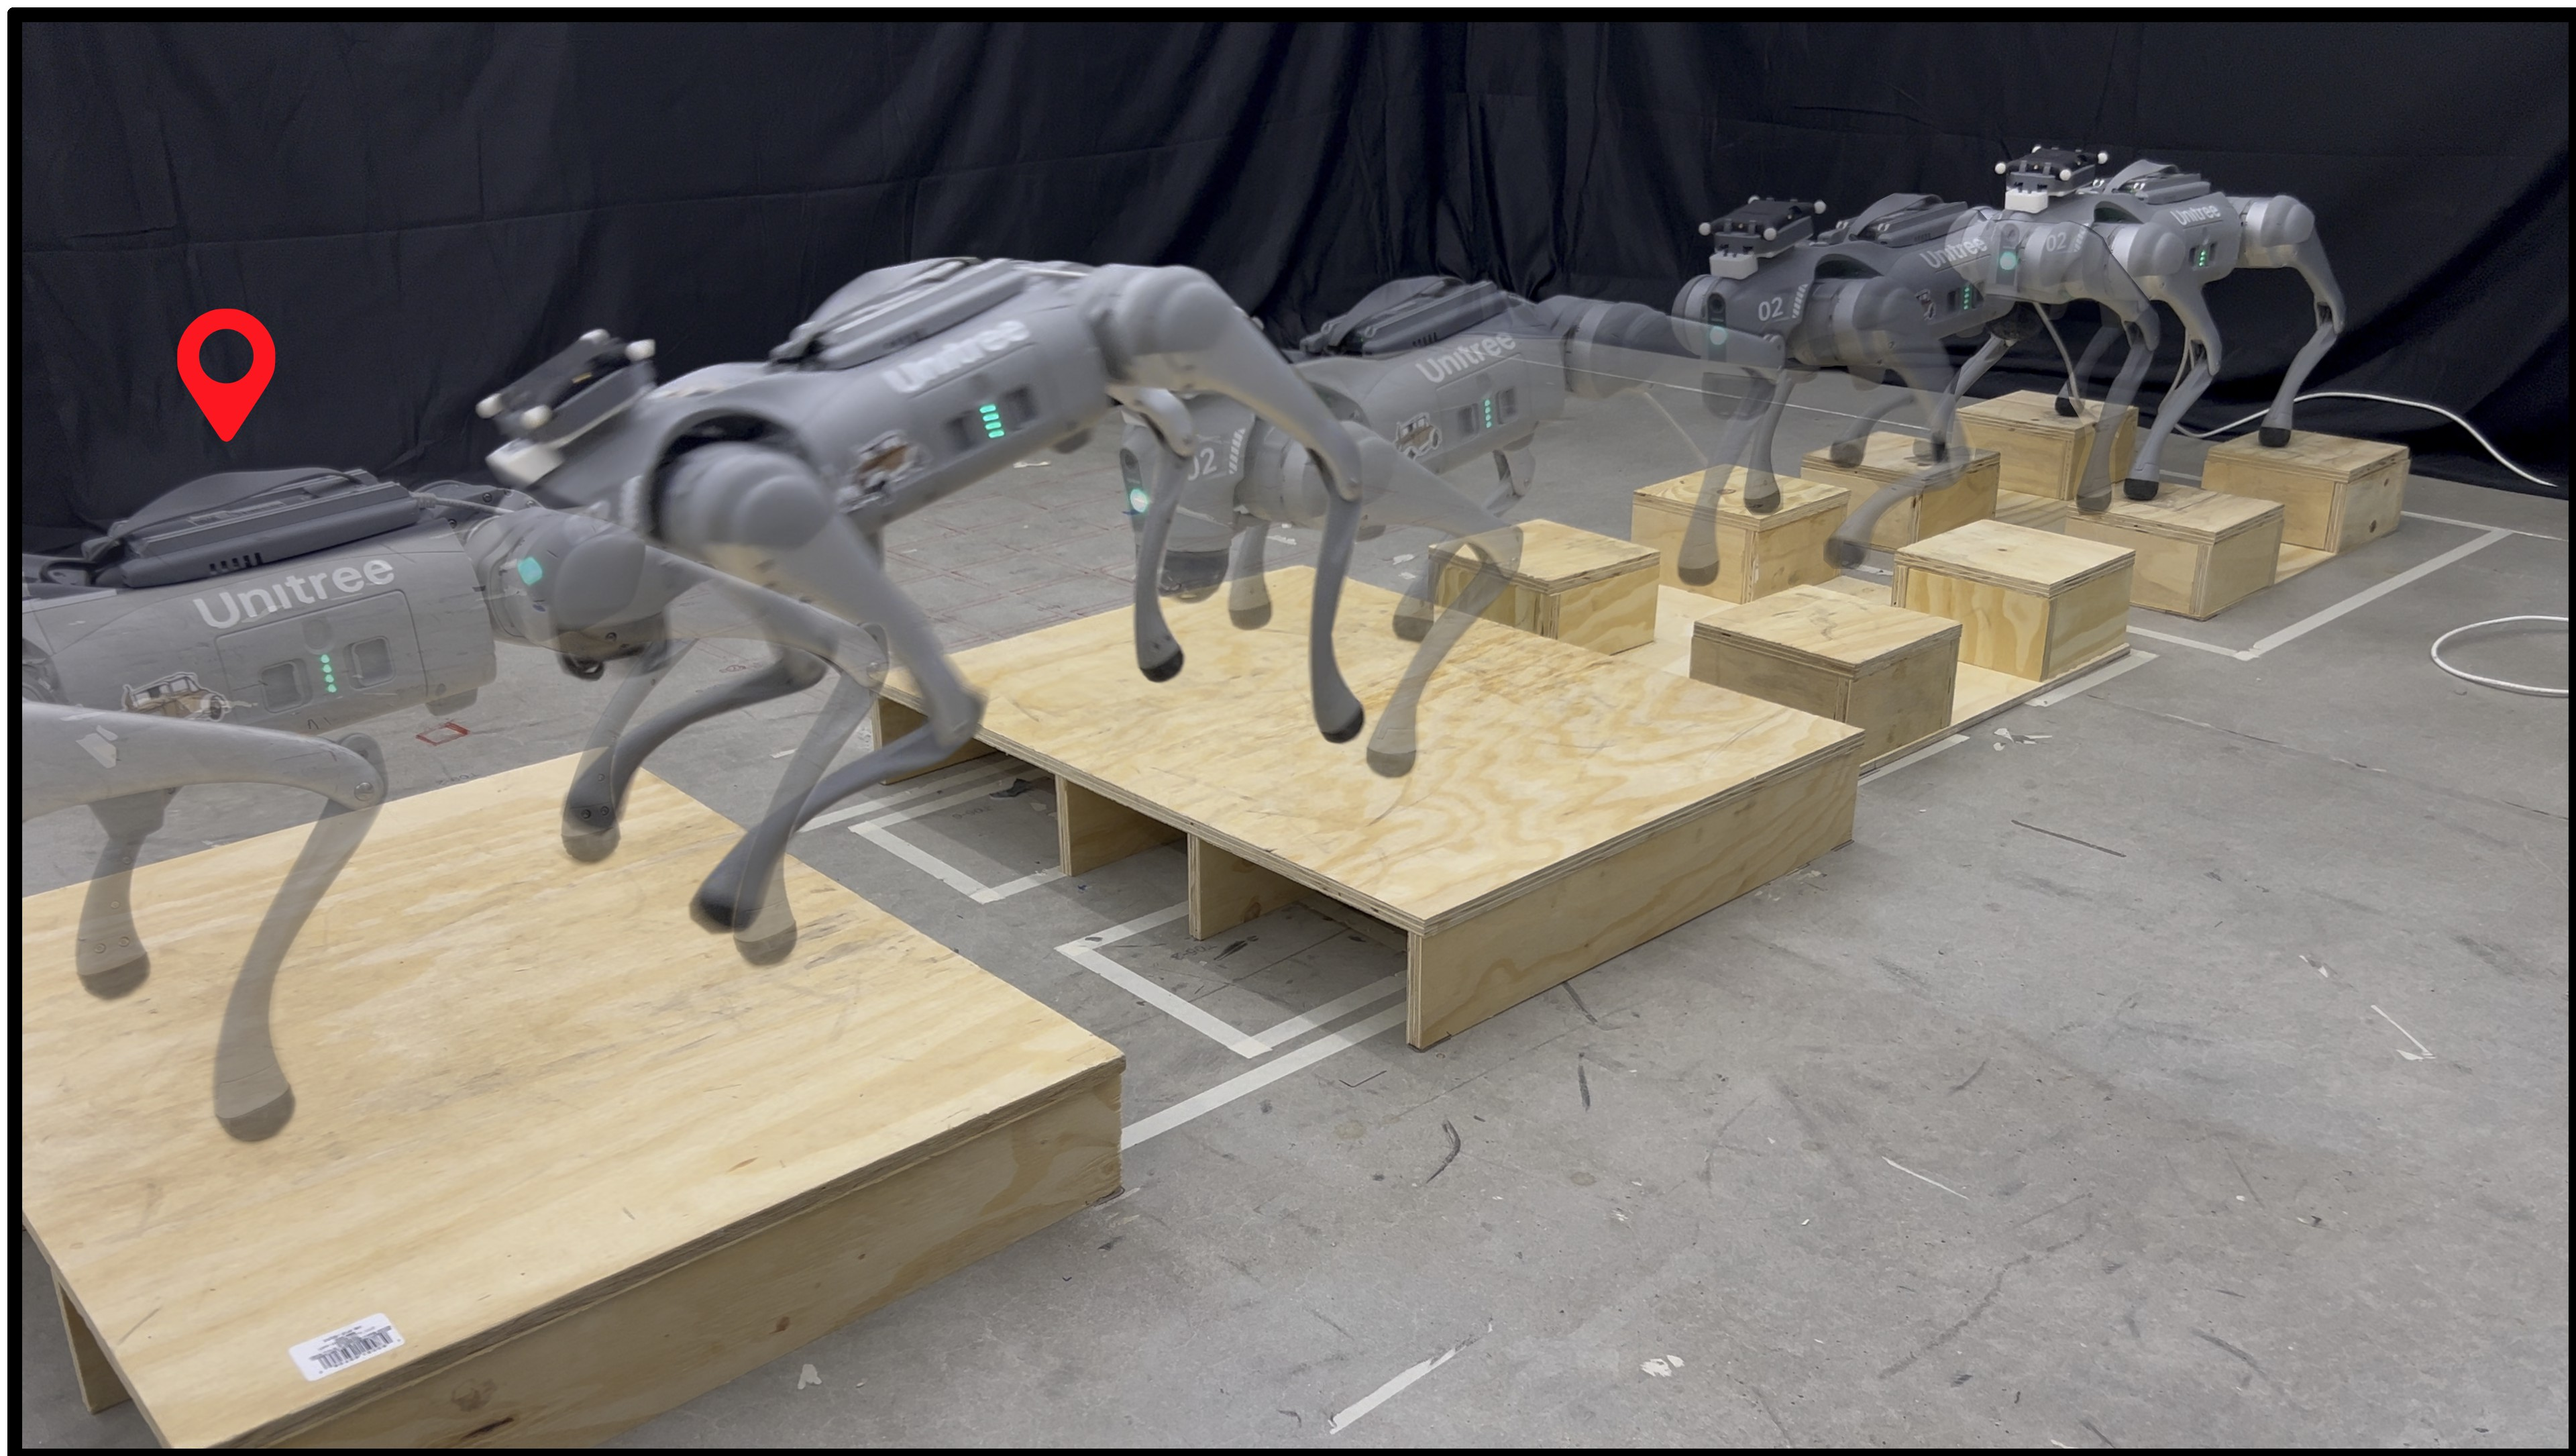
\includegraphics[width=\linewidth]{unstructured_hardware_withgap.jpg}
    \caption{Hardware experiment demonstration for the second unstructured terrain scenario with sparse stepping stones, flat, and gap terrains.}
    \label{fig:hardware_withgap}
\end{figure}
\begin{figure}
    \centering    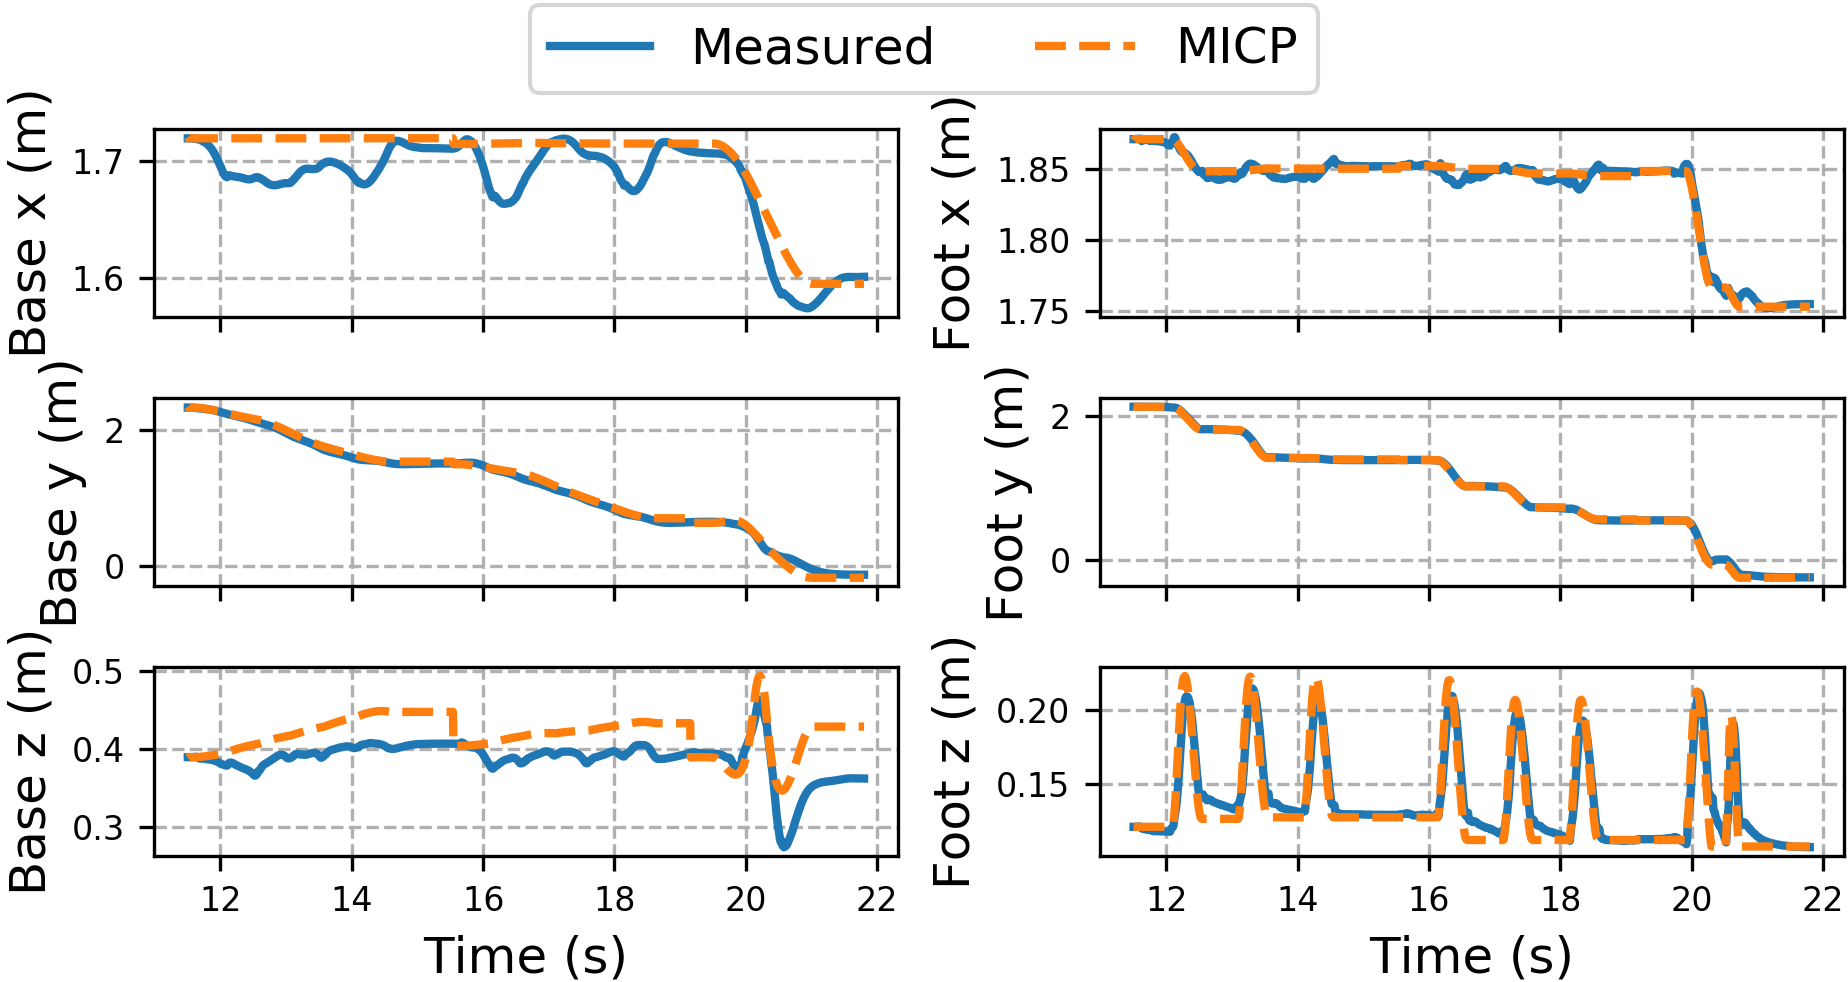
\includegraphics[width=\linewidth]{tracking_performance.png}
    \caption{Tracking performance of the base and front-left foot positions: comparison between measured states and MICP-generated reference trajectories.}
    \label{fig:tracking_performance}
\end{figure}
\subsection{Rebar Terrain}\label{subsec:rebar_terrain}
\begin{figure*}[t]
    \centering
    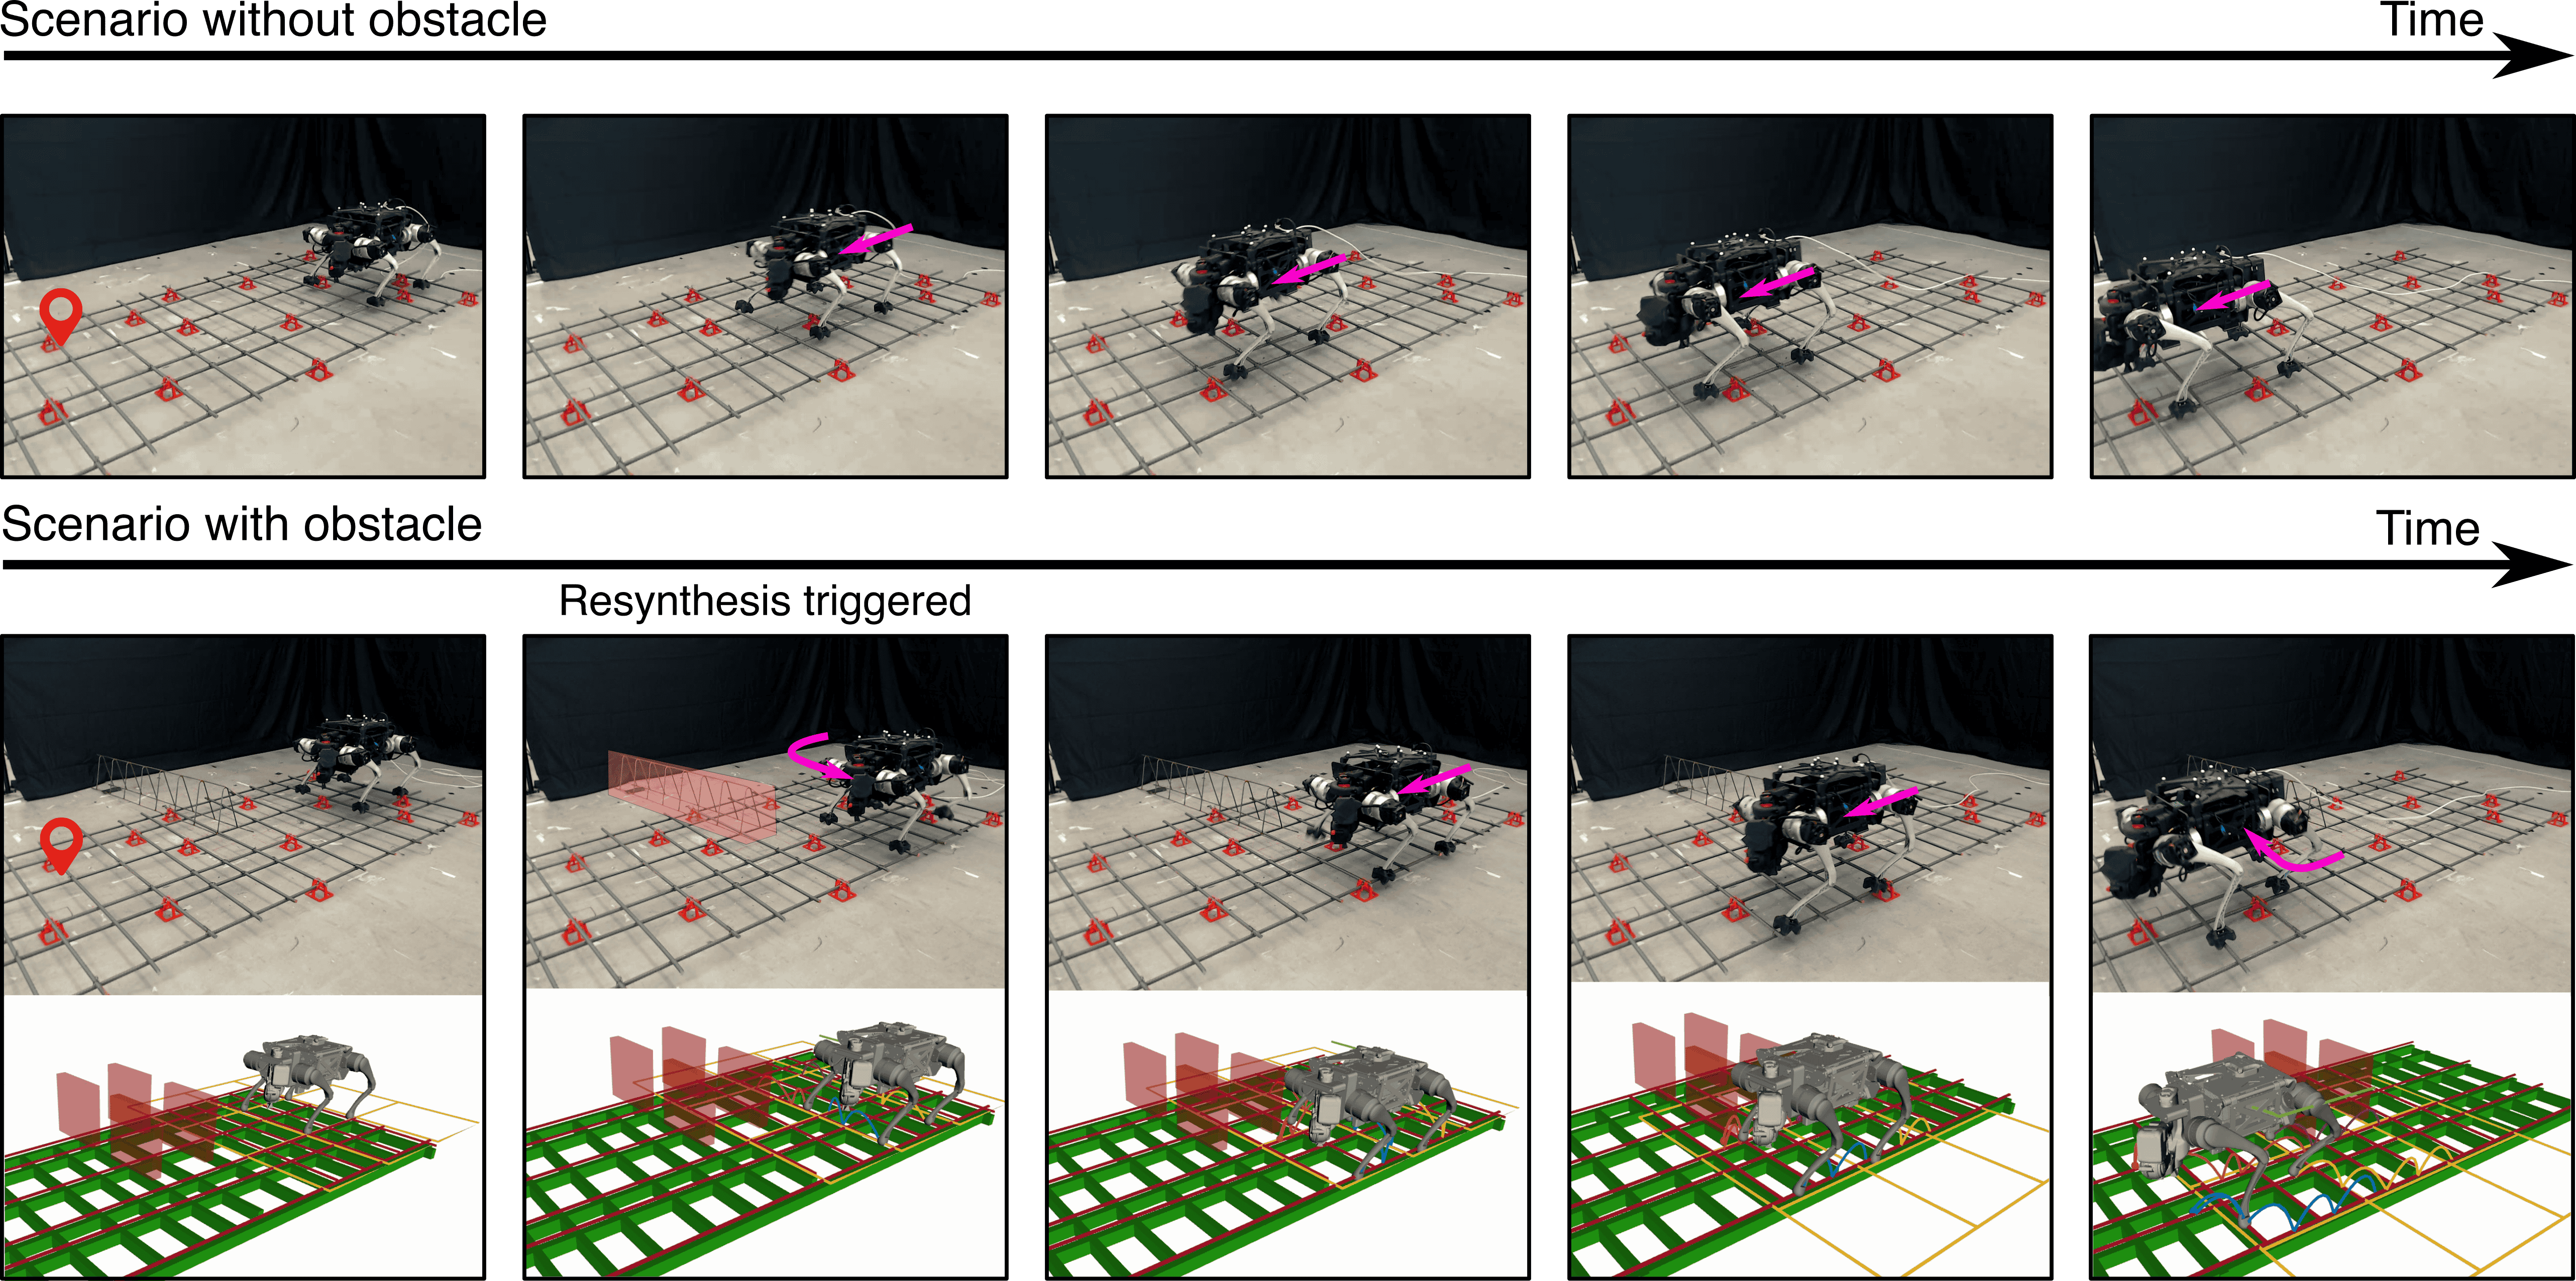
\includegraphics[width=\linewidth]{hardware_rebar_compressed.png}
    \caption{Execution results in rebar terrain without (top row) and with obstacle (bottom row). In the obstacle case, runtime resynthesis is triggered to generate a detour strategy and ensure successful traversal.}
    \label{fig:hardware_rebar}
\end{figure*}
For the rebar terrain scenarios shown in Fig.~\ref{fig:hardware_rebar}, we test two cases: one without any obstacles and one with an obstacle introduced during execution. The rebar spacing varies between $0.1$ m and $0.3$ m. Offline synthesis is conducted without prior knowledge of obstacles. In the first case (top row), the robot Chotu successfully performs the entire maneuver without encountering any runtime failures, consistently moving forward until reaching the goal waypoint.
In the second case (bottom row), an obstacle is added to the environment but only detected during the online execution phase. \revised{In our hardware setup, the obstacle's location is not estimated by an autonomous perception stack but rather provided through motion-capture-aided manual annotation: when the obstacle enters the robot's local field of view, its position is added to the online terrain set and the affected cell is classified as the \textit{obstacle} terrain class at the symbolic level---i.e., obstacle avoidance in this scenario is handled entirely at the symbolic level (Sec.~\ref{sec:preliminaries_abstraction}), not through the MICP-level collision-region variables $\v H_{s,w,j}$ in Eq.~(\ref{eq:collision_avoidance}). This setup is explicit about what is and is not validated---the planning and runtime-repair pipeline is exercised end-to-end, while the terrain-segmentation problem itself is not.} Upon encountering a new terrain/request pair caused by the obstacle, the planner promptly triggers a runtime resynthesis. Leveraging previously generated skills, it computes a new strategy within $0.05$ s to detour around the obstacle and continue toward the goal. All transitions in both scenarios use a $2.25$ s static walking gait, where only one foot is lifted at a time to ensure safety. \revised{We note that the gait timings adopted on hardware---$3$\,s trotting, $1.5$\,s leaping, $2.25$\,s static walking---are conservative compared to the most agile motions reported in the legged-locomotion literature; however, this locomotion gait setup still verifies the framework's gait-switching, online MICP, and runtime-repair mechanisms, which is the validation target of this article. Aggressive, high-speed gaits would require revisiting the convex-dynamics simplification (Eq.~(\ref{eq:dynamics})) discussed in Sec.~\ref{sec:online_execution}.}


\subsection{Benchmark: Heuristics-Based Planner}
\begin{figure*}
    \centering
    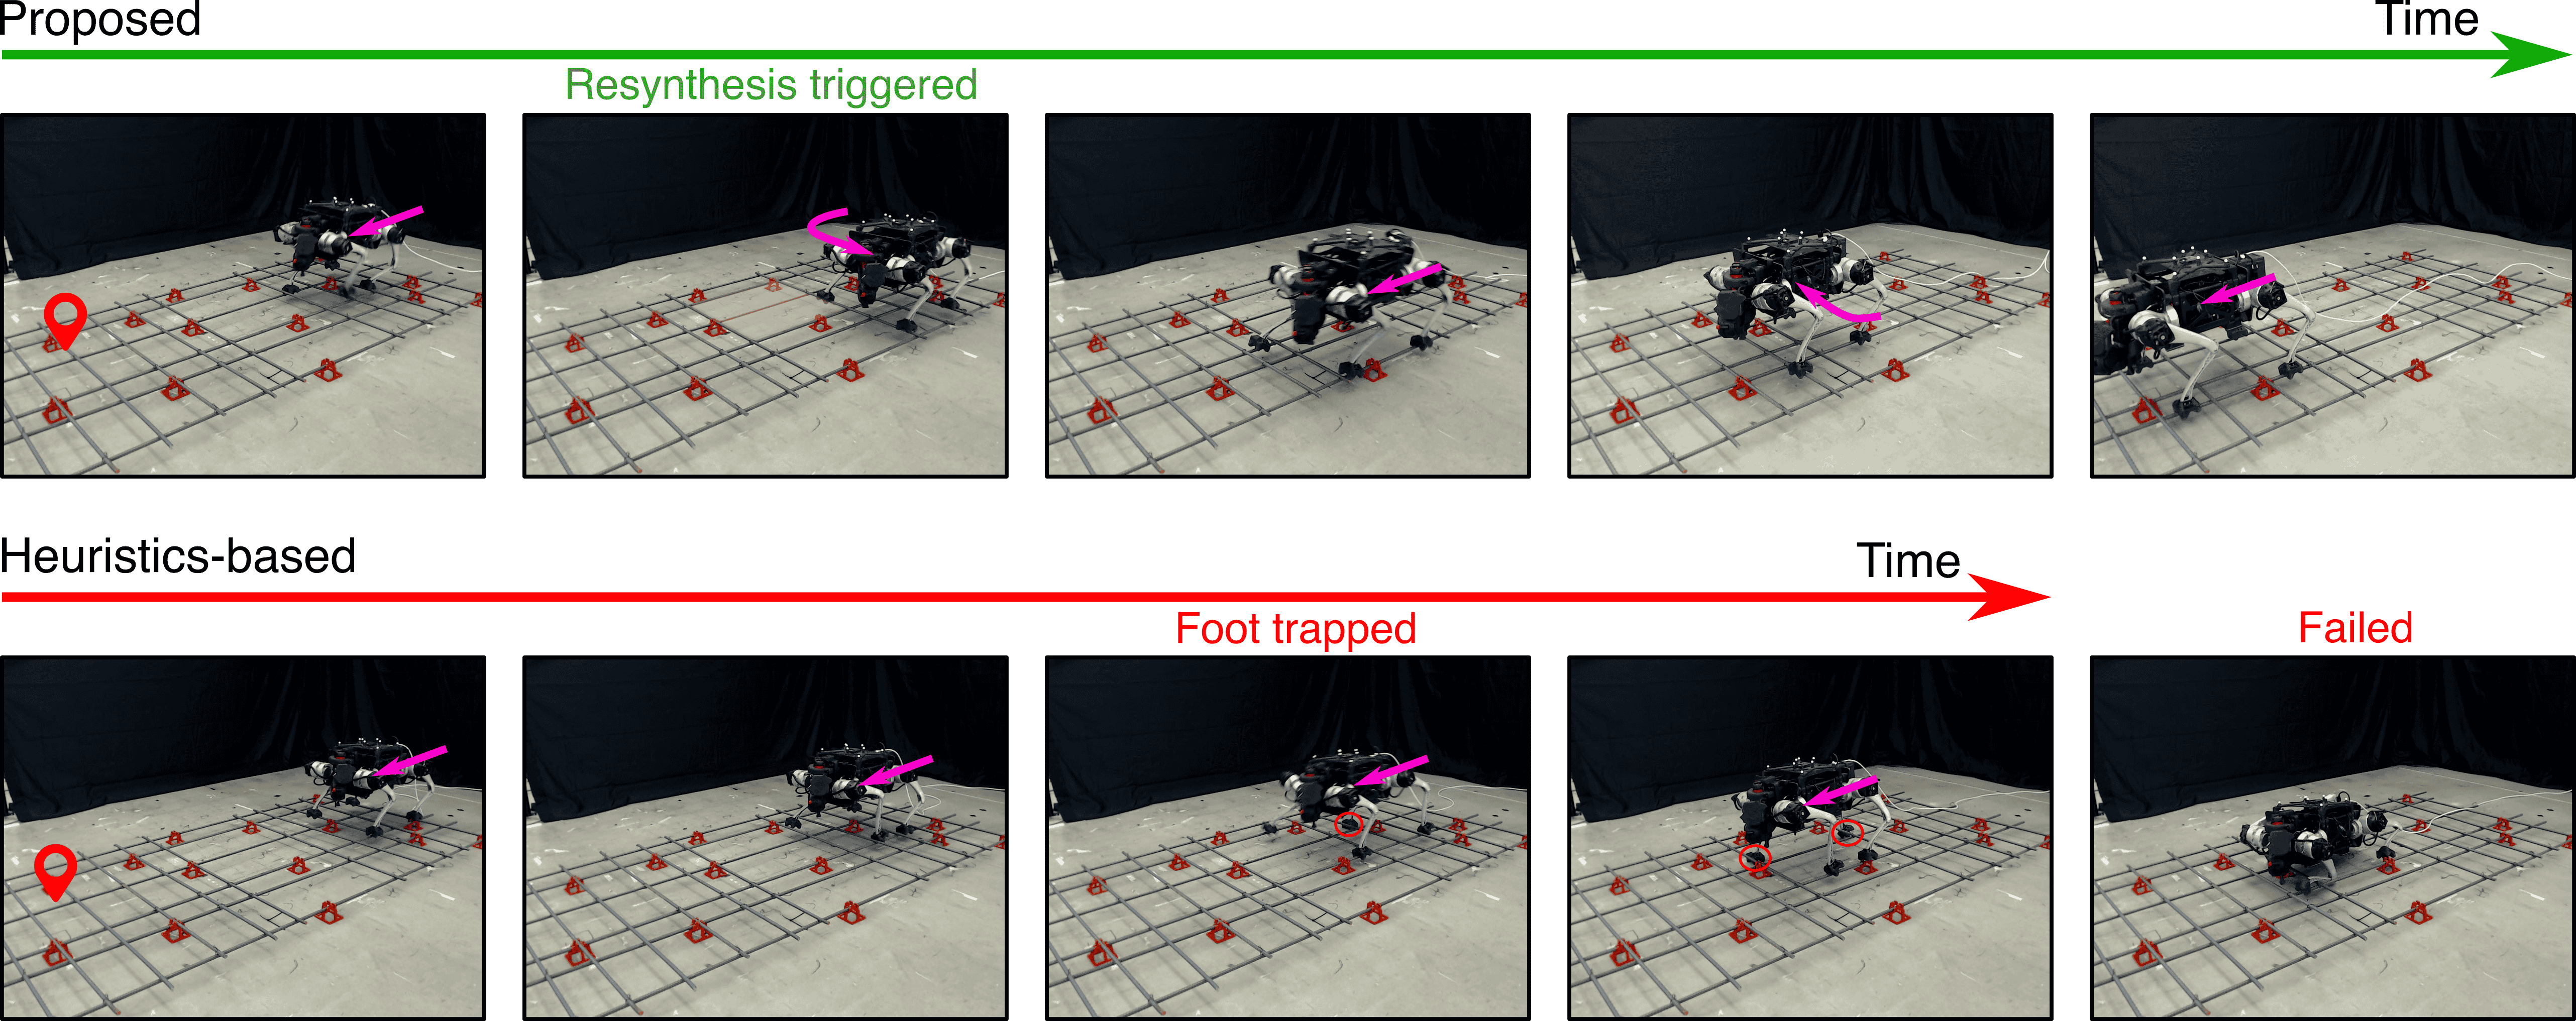
\includegraphics[width=\linewidth]{hardware_rebar_benchmark_compressed.png}
    \caption{Comparison between the proposed method and a heuristics-based planner in an extreme sparse rebar scenario. The proposed method performs resynthesis and succeeds, while the heuristics-based planner fails due to foot trapping.}
    \label{fig:hardware_rebar_benchmark}
\end{figure*}
We create a third rebar scenario, shown in Fig.~\ref{fig:hardware_rebar_benchmark}, by removing two rebars to further increase the maximum spacing to $0.48$ m. This highlights the safety advantage of our planner compared to a heuristics-based footstep planner. The heuristic baseline follows a similar strategy to \citep{fankhauser2018robust, kim2020vision}, adapted for the rebar scenario by selecting the nearest rebar polygon and the closest feasible foothold to a nominal target. The resulting footstep plan and linearly interpolated base trajectory are sent to the same tracking control module. For fairness, all parameters are tuned to achieve successful traversal at a speed of $0.1$ m/s (as shown in the supplemental video).

\revised{We chose this nearest-feasible-foothold heuristic because it isolates the value of feasibility-aware, longer-horizon planning over a single-step heuristic, and because such heuristics remain widely used in deployed perceptive-locomotion stacks due to its computational efficiency. Comparisons against more sophisticated baselines are discussed as future work in Sec.~\ref{sec:discussion}.}

Without re-performing the offline synthesis, our framework directly uses the results from Sec.~\ref{subsec:rebar_terrain}. It classifies the extreme sparse region as an obstacle and performs runtime resynthesis, generating a detour to safely reach the goal. In contrast, we task the heuristics-based planner with the same goal at $0.2$ m/s to match our planner's effective gait speed (i.e., 0.45 m per 2.25 s transition). Without reasoning about the compatibility between terrain geometry and gait feasibility, the heuristic planner suffers from poor EE tracking after a few steps, leading to foot slippage and eventual failure as the robot is entangled by the sparse rebar layout.

\subsection{Computational Time}
We report the hardware computational time in Table~\ref{tab:micp_speed_hardware}. Except for the second scenario in the unstructured terrain, we observe a notable increase in solve time compared to simulation. This is mainly due to two factors: (1) In the first unstructured terrain scenario, the two sets of stepping stones are laterally misaligned from the robot’s viewpoint, requiring non-trivial deviation from the nominal foot location and sideways movement; %\ye{[Does the robot really have a sideway move? It is bit hard to tell in the video.]}\ziyi{[I rephrased it.]} 
(2) In the rebar scenarios, the real-world rebar polygons are not perfectly aligned with the x or y-axis as in simulation, introducing additional numerical complexity for branch-and-bound solvers. Further acceleration of MIP solving through tighter convex relaxations \citep{marcucci2024shortest, lin2024accelerate} remains an important direction for future work.
\begin{table}
\centering
\scriptsize
    \caption{Online Gait-Fixed MICP Solving Time for Hardware}
    \setlength{\tabcolsep}{4pt}
     \begin{tabular}{lccccc}
         \hline
         \textbf{Scenario} &
         \textbf{Polygons} &
         \textbf{Min (s)} &
         \textbf{Mean (s)} &
         \revised{\textbf{Std (s)}} &
         \textbf{Max (s)}\\\hline
         Unstructured - Scene 1 & 6 & 0.81 & 4.04 & \revised{2.50} & 7.86\\
         Unstructured - Scene 2 & 5 & 0.16 & 0.53 & \revised{0.25} & 0.96\\\hline
         Rebar - Scene 1 & 8 & 3.88 & 6.54 & \revised{2.20} & 9.26\\
         Rebar - Scene 2 & 7.5 & 3.60 & 9.13 & \revised{5.50} & 19.23\\
         Rebar - Scene 3 & 6.33 & 2.45 & 7.37 & \revised{4.41} & 14.7\\\hline
    \end{tabular}
    \label{tab:micp_speed_hardware}
\end{table}

%%%%%%%%% Conclusion %%%%%%%%
\section{Discussion}\label{sec:discussion}
\subsection{Generalization to More Types of Terrain}
The current framework relies on manual terrain abstraction and classification, which requires expert knowledge to define terrain types and assign them to discrete symbolic categories. This process typically involves analyzing physical features such as terrain shape, height variation, and support area to determine whether a terrain segment should be labeled as flat, sparse, dense, high, gap, etc. While effective, this expert-driven approach may limit scalability and generalization to novel environments or terrain conditions. Future extensions could incorporate data-driven terrain classification and generation methods, such as supervised learning or clustering based on 3D point cloud statistics to automate the terrain abstraction process and reduce reliance on human heuristics.

\subsection{Optimality}
The synthesis process focuses on guaranteeing feasibility and correctness of transitions but does not account for the relative cost or quality of different feasible gaits. When multiple locomotion gaits (e.g., trotting, bounding, leaping) are viable for a given symbolic transition, the current method does not evaluate their optimality in terms of energy efficiency, robustness, execution time, or other performance metrics. Instead, it selects the first gait that satisfies the physical feasibility conditions via MICP. Integrating cost-aware synthesis would enable the framework to prioritize higher-quality behaviors and make more informed decisions under trade-offs.

\subsection{Perception Module}
The proposed framework is modular and can be directly integrated with a wide range of perception pipelines that provide terrain geometry in the form of segmented polygonal regions \citep{miki2022elevation}. Existing perception modules that perform terrain segmentation using LiDAR, RGB-D sensors, or stereo vision can be adapted to supply the required input to the MICP planner and symbolic abstraction layers. \revised{In this work we deliberately treated the perception layer as out of scope and used motion-capture-aided manual labeling on hardware (Sec.~\ref{sec:hardware}); a fully autonomous deployment will need to address how perception uncertainty---segmentation noise, polygon misalignment, and per-frame perception delay---propagates through the MICP feasibility certificates and the symbolic-level realizability guarantees. In the current framework, runtime symbolic repair already provides a partial fallback: when perceived terrain causes the symbolic specification to become unrealizable, repair triggers and synthesizes new skills. Quantifying the resilience of this fallback under realistic perception noise is an important next step.}

\revised{\subsection{Reactivity and Update Frequencies}
Across the experiments reported in this article, the symbolic strategy automaton evolves at the timescale of one symbolic transition, which corresponds to one online MICP solve---typically hundreds of milliseconds to a few seconds (Tables~\ref{tab:micp_speed} and~\ref{tab:micp_speed_hardware}). Two complementary directions exist for tightening this loop in future work.

First, more frequent MICP updates---e.g., re-solving the online gait-fixed MICP at every NMPC tick rather than once per symbolic transition---are easily adaptable in the proposed framework: the delay-aware coordination scheme already supports asynchronous MICP solves of arbitrary duration, so any speed-up of the underlying mixed-integer solver, or any per-transition simplification, translates directly into a higher MICP update rate. The current limit is therefore the MICP solve time itself rather than any architectural constraint.

Second, more frequent symbolic-level planning is also achievable but requires careful design of the symbolic abstraction. Higher-frequency symbolic decisions would generally call for a finer abstraction---more atomic propositions per cell, finer terrain or robot-state granularity, or a larger skill repertoire. Reactive synthesis, however, scales exponentially in the number of variables in the specification~\citep{bloem2012synthesis}, so any finer abstraction must be balanced against synthesis cost. The high-level manager and symbolic repair adopted in this article already mitigate this scalability barrier; pushing toward truly real-time symbolic planning is an interesting future direction at the abstraction level rather than a limit of the framework itself.}

\revised{\subsection{Stronger Baseline Comparisons as Future Work}
The experimental validation in this article compares against a pure-MIP planner and a nearest-feasible-foothold heuristic. Two stronger comparison points that we did not implement here remain valuable future targets: (i) optimization-based planners such as TOWR-style phase-based end-effector parameterization~\citep{winkler2018gait}, which jointly optimize gait timing and footholds in continuous time; and (ii) end-to-end perceptive reinforcement-learning controllers, in particular parkour-style policies such as~\citep{zhuang2023robot,hoeller2023anymal,cheng2024extreme,luo2024pie}. A fair comparison against these two methods requires either equipping them with an additional discrete terrain selection mechanism or a comparable high-level navigation layer, which we did not pursue in the present validation.}

\revised{\subsection{Extension to Bipedal and Other Platforms}
This article focuses on quadrupedal locomotion. The framework's symbolic-level machinery---terrain abstraction, GR(1) specifications, symbolic manager, symbolic repair, runtime repair---is platform-agnostic and applicable directly to other systems such as bipedal robots. The MICP layer requires more careful adaptation: angular-momentum modulation becomes critical even at moderate speeds---a regime where the convex-dynamics simplification adopted here (Eq.~(\ref{eq:dynamics})) becomes a stronger limitation. Generalizing to humanoids would also require revisiting the kinematic-feasibility re-targeting MICP to account for arm-swing and balance constraints. We see this as a future direction.}


\section{Conclusion}
% In this work, we presented an integrated planning framework for terrain-adaptive locomotion that combines reactive synthesis with MICP, enabling safe and reactive responses in dynamically changing environments. 
% To address unrealizable specifications arising from limited motion primitives, we introduced a symbolic repair approach that incorporates dynamic feasibility checks, automatically identifying missing transitions necessary for navigating adversarial terrains. In the online execution phase, we tackled the disparity between offline synthesis and real-world conditions by using an online MICP solver and an online symbolic repair process based on real-world terrain data. New terrain conditions encountered during execution. 
% Our approach not only enhances motion feasibility and safety but also provides a scalable solution for legged robots maneuvering in complex and safety-critical environments. Future work will involve extensive hardware testing to validate the proposed framework in real-world scenarios. Additionally, we plan to explore specifications of greater complexity to further test the algorithmic scalability.
In this work, we presented an integrated planning framework for terrain-adaptive locomotion that combines reactive synthesis with MICP, enabling safe and reactive responses in dynamically changing environments. 
To address unrealizable specifications arising from limited motion primitives, we introduced a symbolic repair approach that incorporates dynamic feasibility checks, automatically identifying missing transitions necessary for navigating adversarial terrains. In the online execution phase, we tackled the disparity between offline synthesis and real-world conditions by using an online MICP solver and a runtime repair process based on real-world terrain data, including unforeseen terrain conditions. 
Our approach not only enhances motion feasibility and safety but also provides a scalable solution for legged robots maneuvering in complex and safety-critical environments. 
%

% \section{Acknowledgment}
% We thank Eohan George and Suphakorn Lertruchtkul for their hardware support on Chotu and contributions to rebar scenario design, and Pengyuan Shu for constructing the real-world terrains.

\begin{acks}
We thank Eohan George, Suphakorn Lertruchtkul, and Jane Ivanova for their hardware support on Chotu and contributions to rebar scenario design, and Pengyuan Shu for constructing the real-world terrains. The authors would also like to thank Hemanth Surya for the early exploration of the terrain segmentation.
\end{acks}

\begin{aucon}
All authors contributed to the study. Ziyi Zhou: Conceptualization,
Methodology, Formal analysis, Investigation, Software, Project
administration, Writing - original draft. Qian Meng: Methodology, Formal analysis, Investigation Software, Writing - original draft. Hadas Kress-Gazit: Methodology, Supervision, Writing – review and editing. Ye Zhao: Funding acquisition, Resources, Methodology, Supervision, Writing – review and editing. All authors reviewed and approved the final version
of the manuscript.
\end{aucon}

\begin{ethical}
Not applicable.
\end{ethical}

\begin{conpart}
Not applicable.
\end{conpart}

\begin{conpub}
Not applicable.
\end{conpub}

\begin{dci}
The author(s) declared no potential conflicts of interest with respect
to the research, authorship, and/or publication of this article.
\end{dci}

\begin{funding}
The author(s) disclosed receipt of the following financial support
for the research, authorship, and/or publication of this article:
This work was supported
through a sponsored research grant from SkyMul Inc. and a Georgia Tech
IRIM/IPaT Aware Home Seed Grant.
This work was also supported in part by the National
Science Foundation (NSF) under Grant \#CMMI-2144309, and Grant \#FRR-2328254, Office of Naval Research (ONR)
under Grant N000142312223, and in part by the United States Department of Agriculture (USDA) under Grant 2023-67021-41397.
\end{funding}

\bibliographystyle{SageH}
\bibliography{references}

\end{document}
